% Stuff that may change from year to year; also check slide s:other-courses
\newcommand{\coursepath}{/teaching/2021/ConcDisSys}
\newcommand{\courseurl}{\url{https://www.cst.cam.ac.uk\coursepath}}
\newcommand{\thisyear}{2020/21}
\newcommand{\timestampexample}{2020-11-09T09:50:17+00:00}
\newcommand{\whenissecurity}{Part IB Easter term}

% Lecture dates for 2020:
% 2020-11-05
% 2020-11-10
% 2020-11-12
% 2020-11-17
% 2020-11-19
% 2020-11-24
% 2020-11-26
% 2020-12-01
% Instructions for editing course web page: https://www.cl.cam.ac.uk/teaching/2021/instructions.html

\fancypagestyle{plain}{%
  \renewcommand{\headrulewidth}{0pt}%
  \fancyhf{}%
  \fancyfoot[C]{%
      \raisebox{-0.15cm}{
\includegraphics[height=0.5cm]{images/creative-commons.png}}\hspace{5pt}
      This work is published under a \href{https://creativecommons.org/licenses/by-sa/4.0/}{Creative Commons BY-SA license}.%
  }%
}

\begin{document}
\title{Distributed Systems}
\subtitle{University of Cambridge\\Computer Science Tripos, Part IB\\Michaelmas term \thisyear\\\courseurl}

\author{Dr.\ Martin Kleppmann\\mk428@cst.cam.ac.uk}
\date{}
\maketitle

\def\sectionautorefname{Section}%
\def\subsectionautorefname{Section}%
\def\subsubsectionautorefname{Section}%

\section{Introduction}\label{sec:introduction}

\begin{frame}
    \label{s:title}
    \begin{center}
        \textbf{\huge{\color{darkblue}{Distributed Systems}}} \\[2em]
        The second half of \emph{Concurrent and Distributed Systems}\\[0.5em]
        \url{https://www.cl.cam.ac.uk/teaching/current/ConcDisSys}\\[2em]
        Dr.\ Martin Kleppmann (mk428@cam) \\[0.5em]
        University of Cambridge \\[0.5em]
        Computer Science Tripos, Part IB \\[2em]
    \end{center}
    \begin{columns}[totalwidth=9cm]
        \begin{column}{4cm}
            \hfill
\includegraphics[height=0.5cm]{images/creative-commons.png}\hspace{5pt}
        \end{column}
        \begin{column}{5cm}\scriptsize
            This work is published under a\\\href{https://creativecommons.org/licenses/by-sa/4.0/}{Creative Commons BY-SA license}.
        \end{column}
    \end{columns}
\end{frame}

This 8-lecture course on distributed systems forms the second half of \emph{Concurrent and Distributed Systems}.
While the first half focussed on concurrency among multiple processes or threads running on the same computer, this second half takes things further by examining systems consisting of multiple communicating computers.

Concurrency on a single computer is also known as \emph{shared-memory concurrency}, since multiple threads running in the same process have access to the same address space.
Thus, data can easily be passed from one thread to another: a variable or pointer that is valid for one thread is also valid for another.

This situation changes when we move to distributed systems.
We still have concurrency in a distributed system, since different computers can execute programs in parallel.
However, we don't typically have shared memory, since each computer in a distributed system runs its own operating system with its own address space, using the memory built into that computer.
Different computers can only communicate by sending each other messages over a network.

(Limited forms of distributed shared memory exist in some supercomputers and research systems, and there are technologies like \emph{remote direct memory access} (RDMA) that allow computers to access each others' memory over a network.
Also, databases can in some sense be regarded as shared memory, but with a different data model compared to byte-addressable memory.
However, broadly speaking, most practical distributed systems are based on message-passing.)

Each of the computers in a distributed system is called a \emph{node}.
Here, ``computer'' is interpreted quite broadly: nodes might be desktop computers, servers in datacenters, mobile devices, internet-connected cars, industrial control systems, sensors, or many other types of device.
In this course we don't distinguish them: a node can be any type of communicating computing device.

\begin{frame}
    \label{s:dist-sys-definition}
    \frametitle{A distributed system is\dots}
    \begin{itemize}
        \item<1-> \emph{``{\dots}a system in which the failure of a computer you didn't even know existed can render your own computer unusable.''} --- Leslie Lamport\\[1em]
        \item<2> {\dots}multiple computers communicating via a network\dots
        \item<2> {\dots}trying to achieve some task together
        \item<2> Consists of ``nodes'' (computer, phone, car, robot, \dots)
    \end{itemize}
    \hfill\includegraphics<1>[height=4cm]{images/lamport.jpg}
\end{frame}
\inlineslide{s:dist-sys-definition}\label{l:dist-sys-definition}
% reference for Lamport quote: https://www.microsoft.com/en-us/research/publication/distribution/
% License for photo: https://commons.wikimedia.org/wiki/File:Leslie_Lamport.jpg

\subsection{About this course}\label{sec:about}

These notes and the lecture recordings should be self-contained, but if you would like to read up on further detail, there are several suggested textbooks:
\begin{itemize}
    \item Maarten van Steen and Andrew S.\ Tanenbaum. \emph{Distributed Systems}. ISBN 978-1543057386.
        Free download from \url{https://www.distributed-systems.net/index.php/books/ds3/} (third edition, 2017).

        This book gives a broad overview over a large range of distributed systems topics, with lots of examples from practical systems.

    \item Christian Cachin, Rachid Guerraoui, and Luís Rodrigues.
        \emph{Introduction to Reliable and Secure Distributed Programming}.
        Second edition, Springer, 2011. ISBN 978-3-642-15259-7.

        Ebook download for Cambridge users: \url{https://link.springer.com/book/10.1007/978-3-642-15260-3} then click Log in $\rightarrow$ via Shibboleth $\rightarrow$ type \emph{University of Cambridge} $\rightarrow$ log in with Raven.

        This book is more advanced, going into depth on several important distributed algorithms, and proving their correctness.
        Recommended if you want to explore the theory in greater depth than this course covers.

    \item Martin Kleppmann. \emph{Designing Data-Intensive Applications}, O'Reilly, 2017. ISBN 978-1449373320.

        This book goes more in the direction of databases, but also covers a number of distributed systems topics.
        It is designed for software engineers in industry working with distributed databases.

    \item Jean Bacon and Tim Harris. \emph{Operating Systems: Concurrent and Distributed Software Design}.
        Addison-Wesley, 2003. ISBN 978-0321117892.

        This book provides a link to the \emph{concurrent systems} half of the course, and to operating systems topics.
\end{itemize}

Where appropriate, these lecture notes also contain references to research papers and other useful background reading (these are given in square brackets, and the details appear at the end of this document).
However, only material covered in the lecture notes and videos is examinable.

\begin{frame}
    \label{s:reading}
    \frametitle{Recommended reading}
    \begin{itemize}
        \item van Steen \& Tanenbaum.\\ ``\textbf{Distributed Systems}''\\(any ed), free ebook available
        \item Cachin, Guerraoui \& Rodrigues. \\ ``\textbf{Introduction to Reliable and Secure Distributed Programming}'' (2nd ed), Springer 2011
        \item Kleppmann.\\ ``\textbf{Designing Data-Intensive Applications}'',\\O’Reilly 2017
        \item Bacon \& Harris.\\ ``\textbf{Operating Systems: Concurrent and Distributed Software Design}'', Addison-Wesley 2003
    \end{itemize}
\end{frame}
\inlineslide{s:reading}

The syllabus, slides, and lecture notes for this course have been substantially revised for 2020/21.
This means that new mistakes may have crept in.
If you notice anything wrong, or if anything is unclear, please let me know by email (\url{mk428@cst.cam.ac.uk})!

As for other courses, past exam questions are available at \url{https://www.cl.cam.ac.uk/teaching/exams/pastpapers/t-ConcurrentandDistributedSystems.html}.
Because of syllabus changes, some of the past exam questions are no longer applicable.
TODO: details on which questions are obsolete.

These notes also contain exercises, which are suggested material for discussion in supervisions.
Solution notes for supervisors are available from the course web page.

This course is related to several other courses in the tripos, as shown on \autoref{l:other-courses}.

\begin{frame}
    \label{s:other-courses}
    \frametitle{Relationships with other courses}
    \begin{itemize}
        \item \textbf{Concurrent Systems} -- Part IB\\
            (every distributed system is also concurrent)
        \item \textbf{Operating Systems} -- Part IA\\
            (inter-process communication, scheduling)
        \item \textbf{Databases} -- Part IA\\
            (many modern databases are distributed)
        \item \textbf{Computer Networking} -- Part IB Lent term\\
            (distributed systems involve network communication)
        \item \textbf{Further Java} -- Part IB Michaelmas\\
            (distributed programming practical exercises)
        \item \textbf{Security} -- \whenissecurity\\
            (network protocols with encryption \& authentication)
        \item \textbf{Cloud Computing} -- Part II\\
            (distributed systems for processing large amounts of data)
    \end{itemize}
\end{frame}
\inlineslide{s:other-courses}\label{l:other-courses}


\subsection{Pros and cons of distributed systems}\label{sec:pros-cons}

There are a number of reasons for creating distributed systems.
Some applications are \emph{instrinsically distributed}: if you want to send a message from your phone to your friend's phone, that operation inevitably requires those phones to communicate via some kind of network.

Some distributed systems do things that in principle a single computer could do, but they do it \emph{more reliably}.
A single computer can fail and might need to be rebooted from time to time, but if you are using multiple nodes, then one node can continue serving users while another node is rebooting.
Thus, a distributed system has the potential to be more reliable than a single computer, at least if it is well-designed (somewhat contradicting Lamport's quote on \autoref{l:dist-sys-definition})!

Another reason for distribution is for better \emph{performance}: if a service has users all over the world, and they all have to access a single node, then either the users in the UK or the users in New Zealand are going to find it slow (or both).
By placing nodes in multiple locations around the world, we can get around the slowness of the speed of light by routing each user to a nearby node.

Finally, some large-scale data processing or computing tasks are simply \emph{too big} to perform on a single computer, or would be intolerably slow.
For example, the Large Hadron Collider at CERN is supported by a worldwide computing infrastructure with 1 million CPU cores for data analysis, and 1 exabyte ($10^{18}$ bytes) of storage! See \url{https://wlcg-public.web.cern.ch/}.

\begin{frame}
    \label{s:why-distribute}
    \frametitle{Why make a system distributed?}
    \begin{itemize}\pause
        \item \textbf{It's inherently distributed:}\\e.g. sending a message from your mobile phone to your friend's phone\pause
        \item \textbf{For better reliability:}\\even if one node fails, the system as a whole keeps functioning\pause
        \item \textbf{For better performance:}\\get data from a nearby node rather than one halfway round the world\pause
        \item \textbf{To solve bigger problems:}\\e.g. huge amounts of data, can't fit on one machine
    \end{itemize}
\end{frame}
\inlineslide{s:why-distribute}

However, there are also downsides to distributed systems, because things can go wrong, and the system needs to deal with such faults.
The network may fail, leaving the nodes unable to communicate.

\begin{frame}
    \label{s:no-internet}
    
\includegraphics[height=\paperheight]{images/no-internet.png}
\end{frame}
\inlineslide{s:no-internet}

Another thing that can go wrong is that a node may crash, or run much slower than usual, or misbehave in some other way (perhaps due to a software bug or a hardware failure).
If we want one node to take over when another node crashes, we need to detect that a crash has happened; as we shall see, even that is not straightforward.
Network failures and node failures can happen at any moment, without warning.

In a single computer, if one component fails (e.g.\ one of the RAM modules develops a fault), we normally don't expect the computer to continue working nevertheless: it will probably just crash.
Software does not need to be written in a way that explicitly deals with faulty RAM.
However, in a distributed system we often \emph{do} want to tolerate some parts of the system being broken, and for the rest to continue working.
For example, if one node has crashed (a \emph{partial failure}), the remaining nodes may still be able to continue providing the service.

If one component of a system stops working, we call that a \emph{fault}, and many distributed systems strive to provide \emph{fault tolerance}: that is, the system as a whole continues functioning despite the fault.
Dealing with faults is what makes distributed computing fundamentally different, and often harder, compared to programming a single computer.
Some distributed system engineers believe that if you can solve a problem on a single computer, it is basically easy!
Though, in fairness to our colleagues in other areas of computer science, this is probably not true.

\begin{frame}
    \label{s:why-not}
    \frametitle{Why NOT make a system distributed?}
    The trouble with distributed systems:
    \begin{itemize}
        \item Communication may fail (and we might not even know it has failed).
        \item Processes may crash (and we might not know).
        \item All of this may happen nondeterministically.
    \end{itemize}\vspace{1em}\pause
    \textbf{Fault tolerance}: we want the system as a whole to continue working, even when some parts are faulty.\\[1em]
    This is hard.\\[1em]
    Writing a program to run on a single computer is comparatively easy?!
\end{frame}
\inlineslide{s:why-not}


\subsection{Distributed systems and computer networking}\label{sec:networking}

When studying distributed systems, we usually work with a high-level abstraction of the hardware.

\begin{frame}
    \label{s:networking}
    \frametitle{Distributed Systems and Computer Networking}
    We use a simple abstraction of communication:
    \begin{center}
        \begin{tikzpicture}
            \node [circle,fill=red!10,draw] (i) at (0,0) {node $i$};
            \node [circle,fill=red!10,draw] (j) at (6,0) {node $j$};
            \draw [bigarrow] (i) -- node [above] {message $m$} (j);
        \end{tikzpicture}
    \end{center}\pause

    Reality is much more complex:
    \begin{itemize}
        \item \textbf{Various network operators:}\\ eduroam, home DSL, cellular data, coffee shop wifi, submarine cable, satellite\dots\\[1em]
        \item \textbf{Physical communication:}\\ electric current, radio waves, laser, hard drives in a van\dots
    \end{itemize}
\end{frame}
\inlineslide{s:networking}

In this course, we just assume that there is some way for one node to send a message to another node.
We don't particularly care how that message is physically represented or encoded~-- the network protocols, informally known as the \emph{bytes on the wire}~-- because the basic principle of sending and receiving messages remains the same, even as particular networking technologies come and go.
The ``wire'' may actually be radio waves, lasers, a USB thumb drive in someone's pocket, or even hard drives in a van.

\begin{frame}[plain]
    \label{s:snowball}
    \frametitle{Hard drives in a van?!}
    \begin{center}
        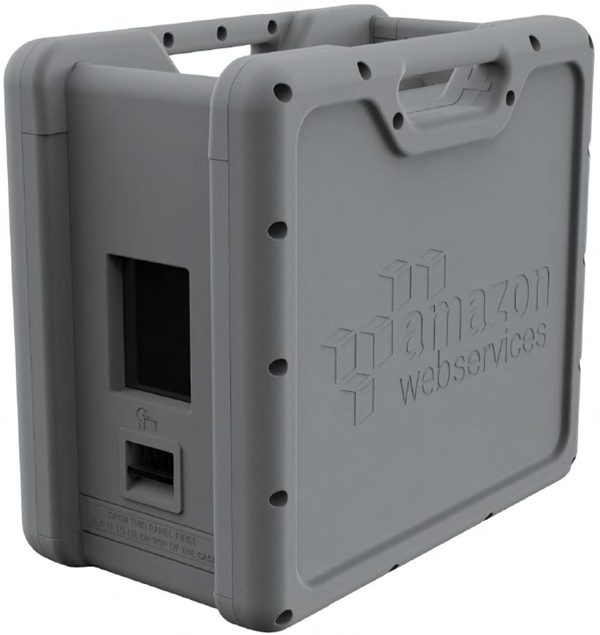
\includegraphics[height=5cm]{images/aws-snowball.png}\\[0.5em]
        \scriptsize{\url{https://docs.aws.amazon.com/snowball/latest/ug/using-device.html}}\\[2em]
        High latency, high bandwidth!
    \end{center}
\end{frame}
\inlineslide{s:snowball}

Indeed, if you want to send a very large message (think tens of terabytes), it would be slow to send that data over the Internet, and it is in fact faster to write that data to a bunch of hard drives, load them into a van, and to drive them to their destination.
But from a distributed systems point of view, the method of delivering the message is not important: we only see an abstract communication channel with a certain \emph{latency} (delay from the time a message is sent until it is received) and \emph{bandwidth} (the volume of data that can be transferred per unit time).

The Computer Networking course in Lent term focusses on the network protocols that enable messages to get to their destination.
The study of distributed systems builds upon that facility, and instead focusses on how several nodes should coordinate in order to achieve some shared task.
The design of distributed algorithms is about deciding what messages to send, and how to process the messages when they are received.

\begin{frame}
    \label{s:latency-bandwidth}
    \frametitle{Latency and bandwidth}
    \textbf{Latency}: time until message arrives
    \begin{itemize}
        \item In the same building/datacenter: $\approx 1$ ms
        \item One continent to another: $\approx 100$ ms
        \item Hard drives in a van: $\approx 1$ day\\[2em]
    \end{itemize}\pause
    \textbf{Bandwidth}: data volume per unit time
    \begin{itemize}
        \item 3G cellular data: $\approx 1$ Mbit/s
        \item Home broadband: $\approx 10$ Mbit/s
        \item Hard drives in a van: 50~TB/box $\approx 1$ Gbit/s\\[1em]
    \end{itemize}
    (Very rough numbers, vary hugely in practice!)
\end{frame}
\inlineslide{s:latency-bandwidth}

\subsection{Example: the web, a client-server distributed system}\label{sec:web}

The web is an example of a distributed system that you use every day.

\begin{frame}[plain]
    \label{s:website}
    \begin{tikzpicture}[remember picture,overlay]
        \node at (current page.center) {
\includegraphics[height=\paperheight]{images/website.png}};
    \end{tikzpicture}
\end{frame}
\inlineslide{s:website}

\begin{frame}
    \label{s:client-server}
    \frametitle{Client-server example: the web}
    Time flows from top to bottom.
    \begin{center}
        \begin{tikzpicture}
            \node [rectangle,fill=red!10,draw] (client) at (0,4) {client};
            \node [rectangle,fill=red!10,draw] (server) at (8,4) {server www.cst.cam.ac.uk};
            \draw (client) -- (0,0);
            \draw (server) -- (8,0);
            \draw<2-> [bigarrow] (0,3) -- node [above,sloped] {GET \coursepath} (8,2);
            \draw<3> [bigarrow] (8,1.5) -- node [above,sloped] {\texttt{<!DOCTYPE html><html>...}} (0,0.5);
        \end{tikzpicture}
    \end{center}
\end{frame}
\inlineslide{s:client-server}

In the web there are two main types of nodes: \emph{servers} host websites, and \emph{clients} (web browsers) display them.
When you load a web page, your web browser sends a \emph{HTTP request} message to the appropriate server.
On receiving that request, the web server sends a \emph{response} message containing the page contents to the client that requested it.
These messages are normally invisible, but we can capture and visualise the network traffic with a tool such as Charles (\url{https://www.charlesproxy.com/}), shown on \autoref{l:http-capture}.

\begin{frame}[plain]
    \label{s:http-capture}
    \begin{tikzpicture}
        \node at (0,0) {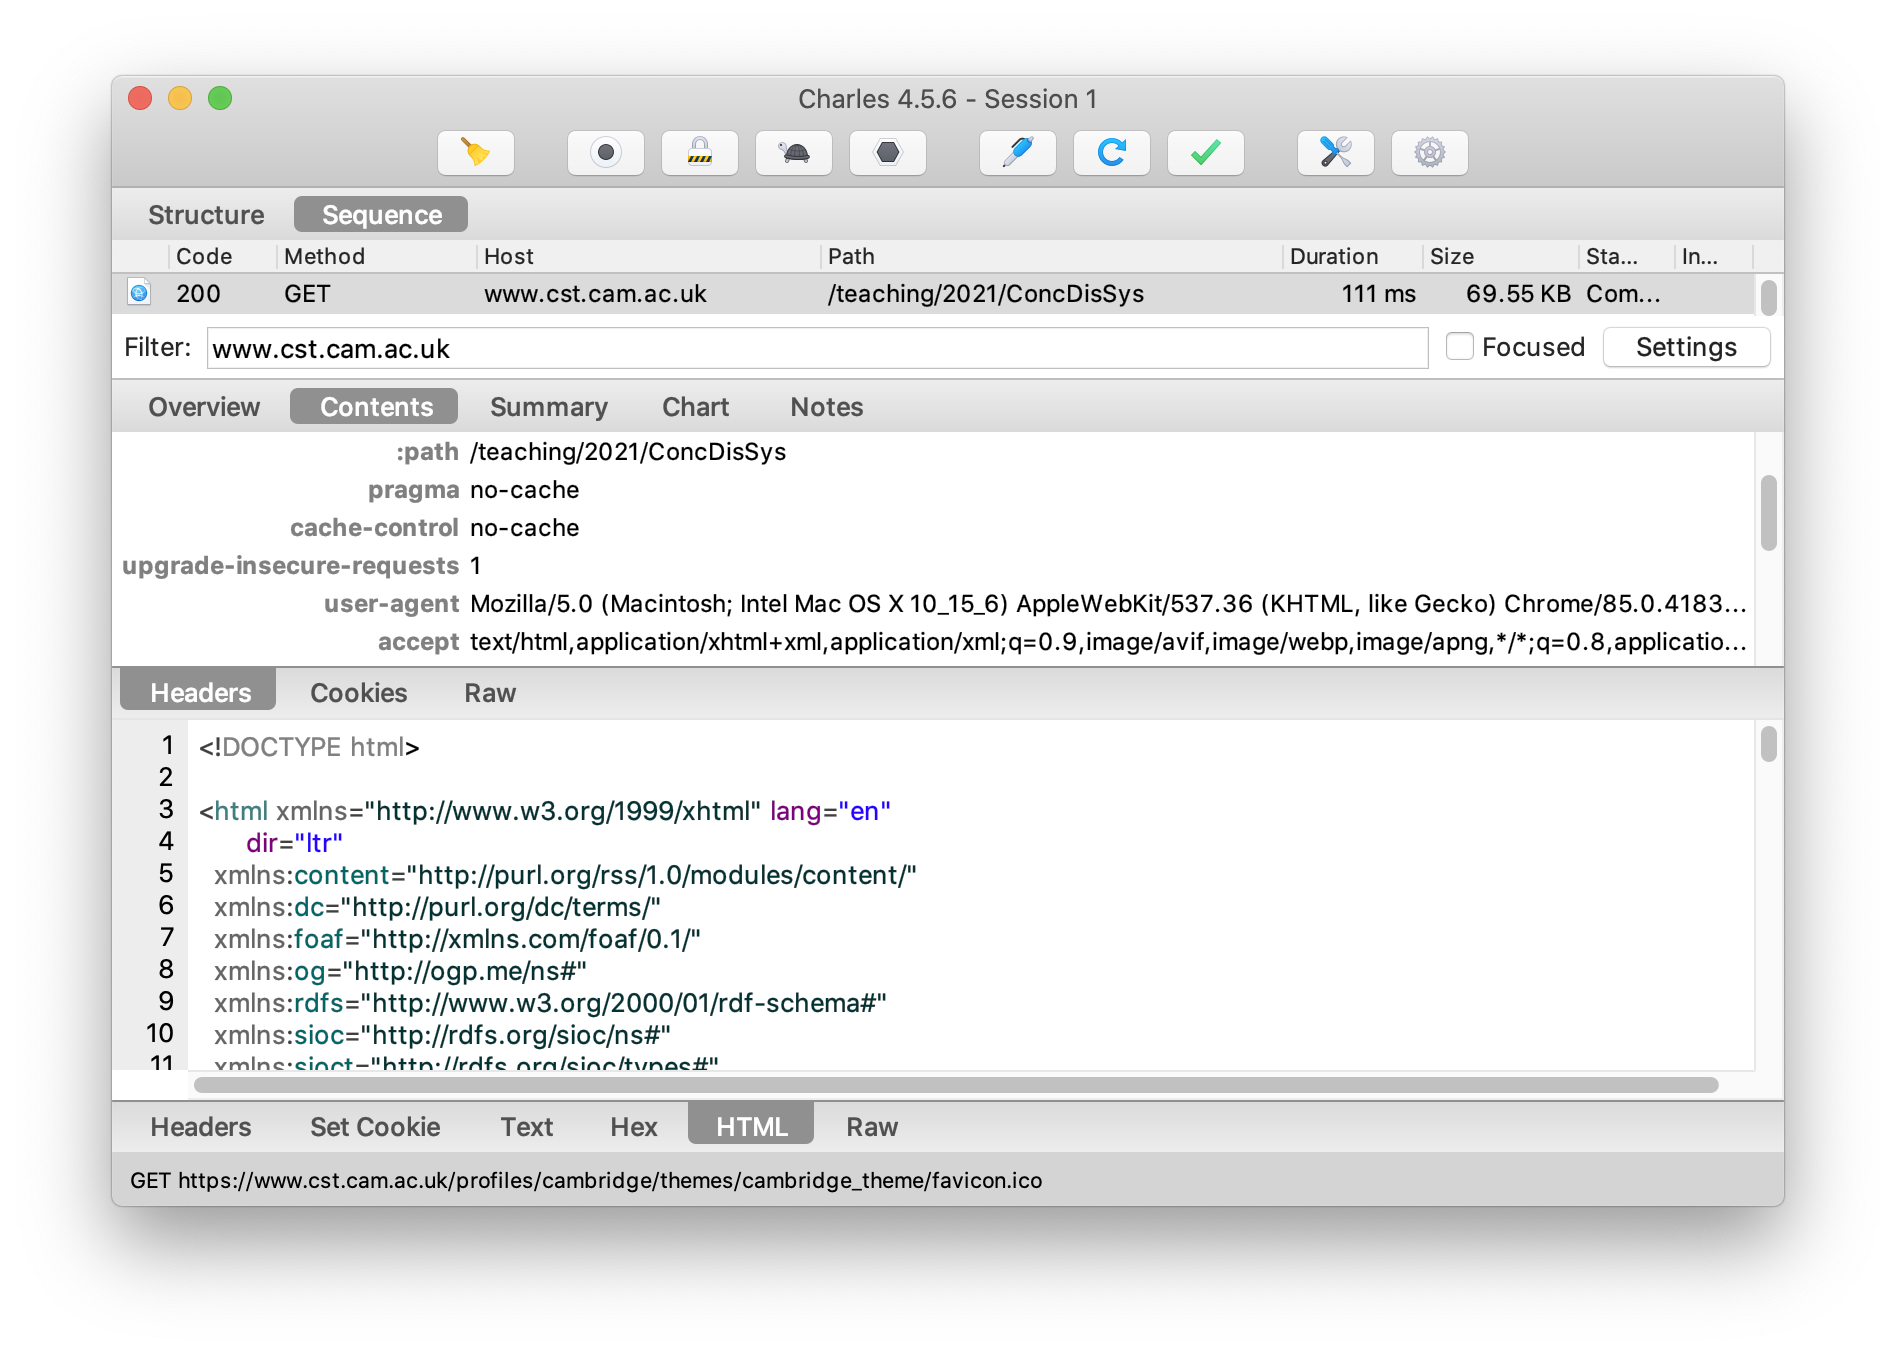
\includegraphics[height=8cm]{images/http-capture.png}};
        \node<2> (request) at (-4,-4.5) [red] {request message};
        \node<2> (response) at (2,-4.5) [red] {response message};
        \draw<2> [-Stealth,red,line width=4pt] (request) -- (-4,0.5);
        \draw<2> [-Stealth,red,line width=4pt] (response) -- (0,-1.2);
    \end{tikzpicture}
\end{frame}
\inlineslide{s:http-capture}\label{l:http-capture}

In a URL, the part between the \verb|//| and the following \verb|/| is the hostname of the server to which the client is going to send the request (e.g.\ \texttt{www.cst.cam.ac.uk}), and the rest (e.g.\ \texttt{\coursepath}) is the path that the client asks for in its request message.
Besides the path, the request also contains some extra information, such as the HTTP method (e.g.\ \texttt{GET} to load a page, or \texttt{POST} to submit a form), the version of the client software (the \emph{user-agent}), and a list of file formats that the client understands (the \emph{accept header}).
The response message contains the file that was requested, and an indicator of its file format (the \emph{content-type}); in the case of a web page, this might be a HTML document, an image, a video, a PDF document, or any other type of file.

Since the requests and responses can be larger than we can fit in a single network packet, the HTTP protocol runs on top of TCP, which breaks down a large chunk of data into a stream of small network packets (see \autoref{l:wireshark}), and puts them back together again at the recipient.
HTTP also allows multiple requests and multiple responses to be sent over a single TCP connection.
However, when looking at this protocol from a distributed systems point of view, this detail is not important: we treat the request as one message and the response as another message, regardless of the number of physical network packets involved in transmitting them.
This keeps things independent of the underlying networking technology.

\begin{frame}[plain]
    \label{s:wireshark}
    \begin{tikzpicture}[remember picture,overlay]
        \node at (current page.center) {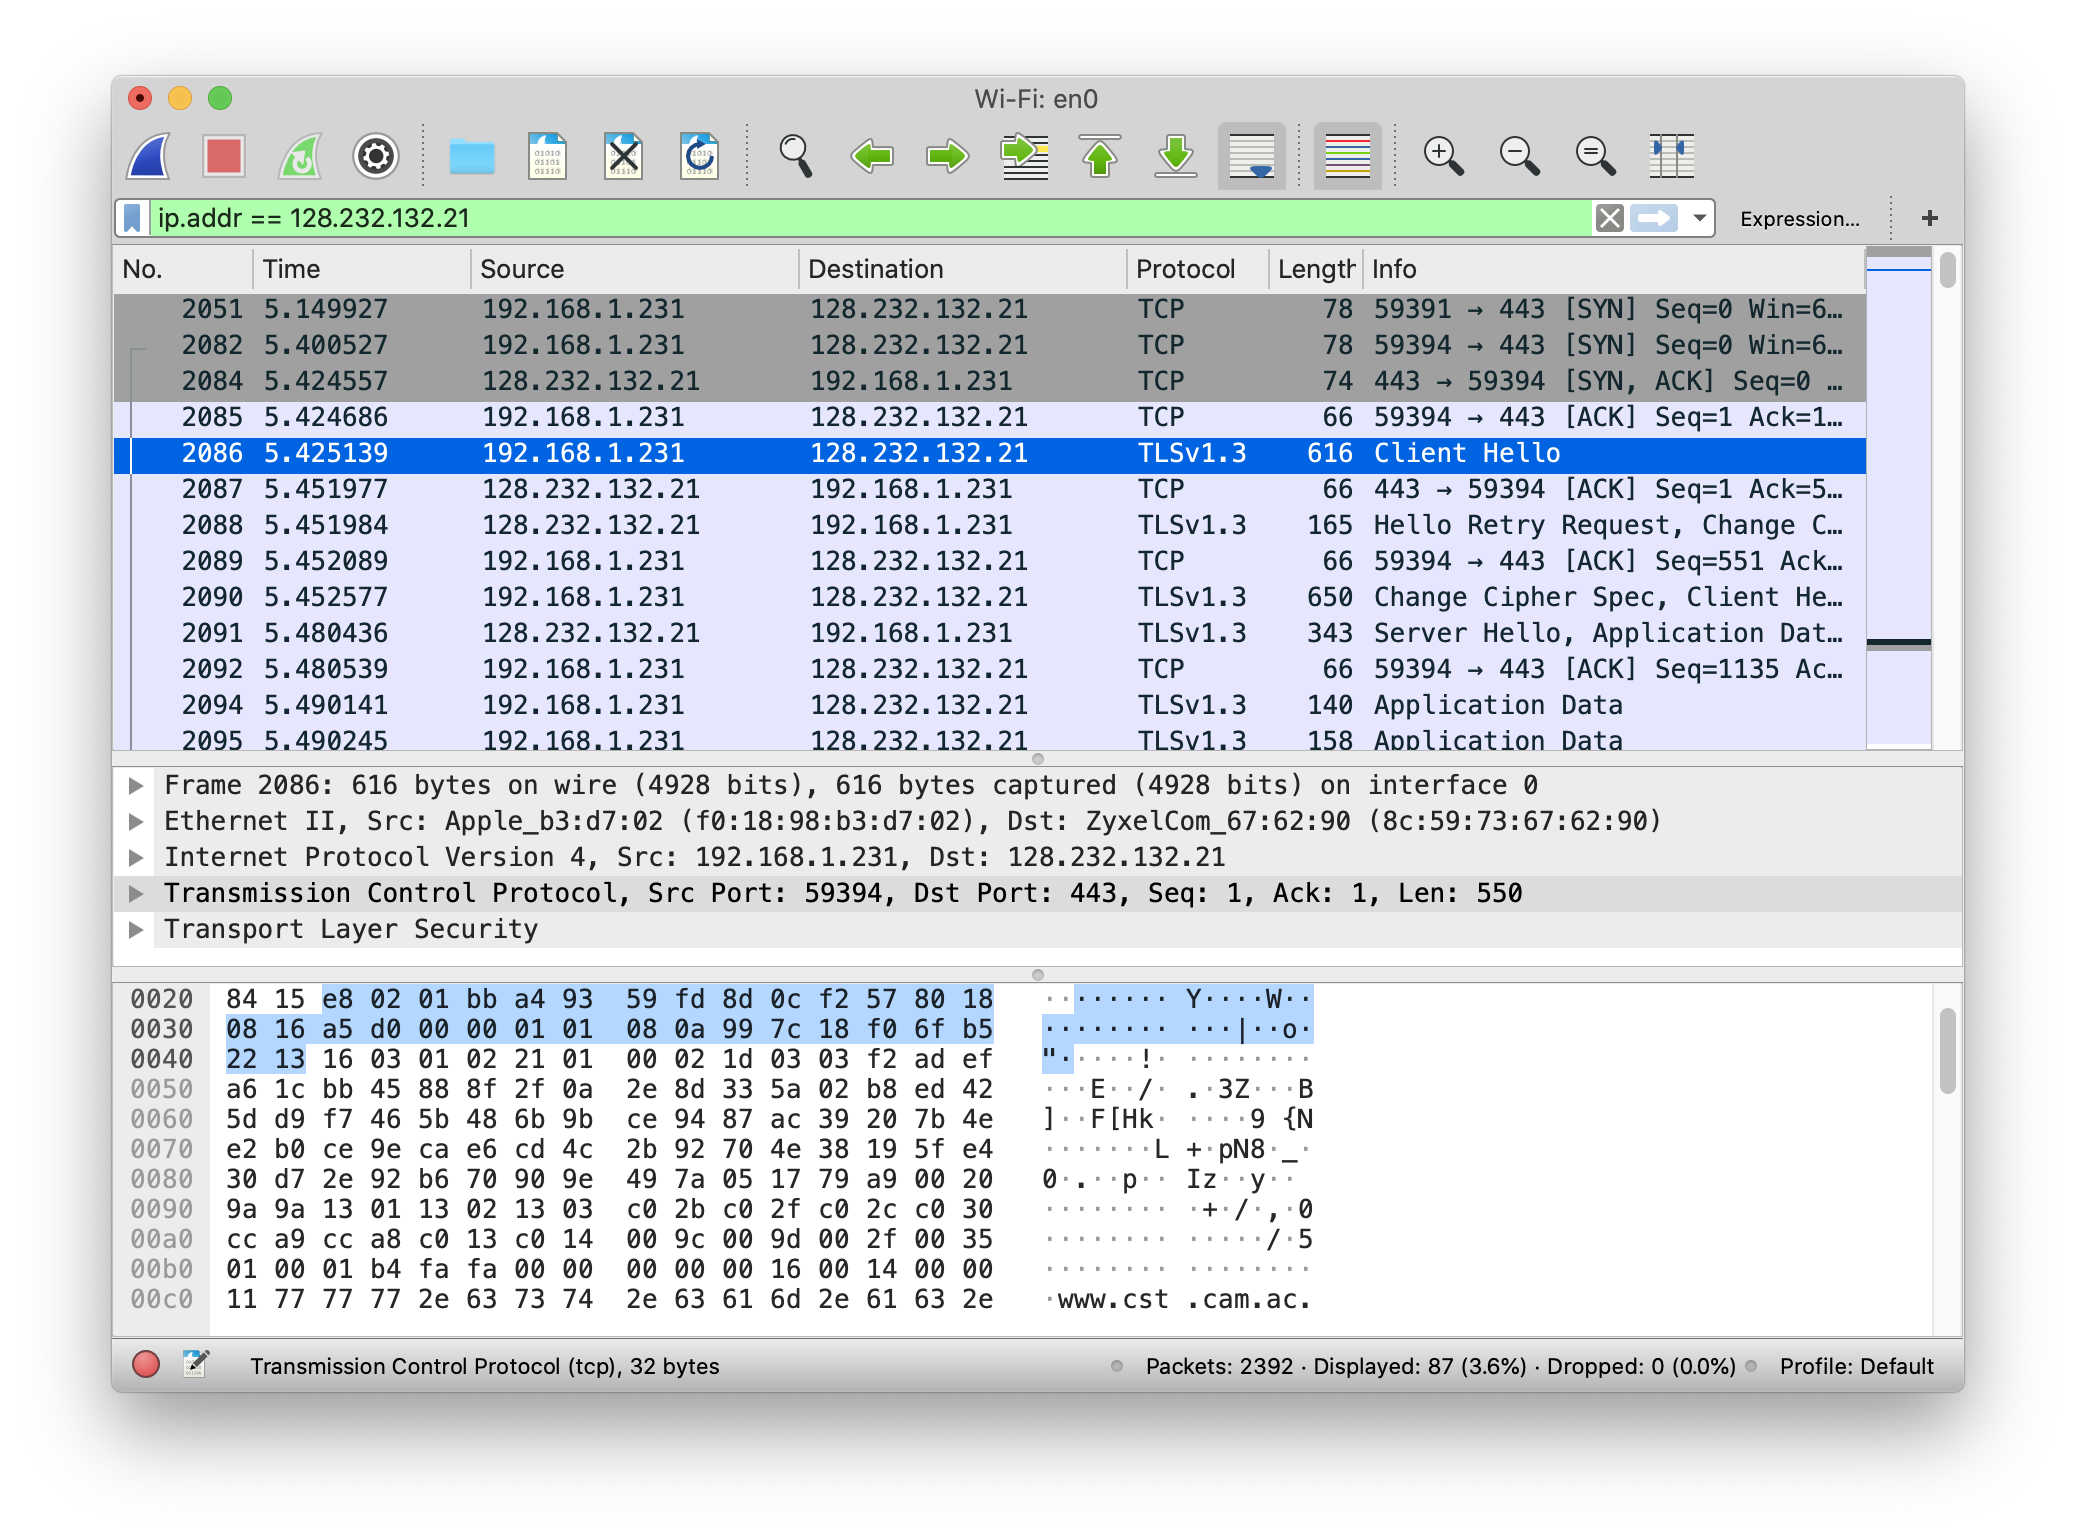
\includegraphics[height=\paperheight]{images/wireshark.png}};
    \end{tikzpicture}
\end{frame}
\inlineslide{s:wireshark}\label{l:wireshark}

\subsection{Example: remote procedure calls (RPC)}\label{sec:rpc}

Another example of an everyday distributed system is when you buy something online using a credit/debit card.
When you enter your card number in some online shop, that shop will send a payment request over the Internet to a service that specialises in processing card payments.

\begin{frame}
    \label{s:payment-example}
    \frametitle{Client-server example: online payments}
    \begin{center}
        \begin{tikzpicture}
            \node [rectangle,fill=red!10,draw] (client) at (0,4) {online shop};
            \node [rectangle,fill=red!10,draw] (server) at (8,4) {payments service};
            \draw (client) -- (0,0);
            \draw (server) -- (8,0);
            \draw<2-> [bigarrow] (0,3) -- node [above,sloped] {charge {\textsterling}3.99 to credit card 1234\dots} (8,2);
            \draw<3> [bigarrow] (8,1.5) -- node [above,sloped] {success} (0,0.5);
        \end{tikzpicture}
    \end{center}
\end{frame}
\inlineslide{s:payment-example}

The payments service in turn communicates with a card network such as Visa or MasterCard, which communicates with the bank that issued your card in order to take the payment.

For the programmers who are implementing the online shop, the code for processing the payment may look something like the code on \autoref{l:payment-rpc}.

\begin{frame}
    \label{s:payment-rpc}
    \frametitle{Remote Procedure Call (RPC) example}
    \inputminted{java}{code/payment-rpc.java}
    \begin{tikzpicture}[remember picture,overlay]
        \node (call) [xshift=2cm,yshift=-0.5cm] at (current page.center) {};
        \node<2> (label) [anchor=south east,red,yshift=0.5cm] at (current page.south east) {Implementation of this function is on another node!};
        \draw<2> [-Stealth,red,line width=4pt] (label) -- (call);
    \end{tikzpicture}
\end{frame}
\inlineslide{s:payment-rpc}\label{l:payment-rpc}

Calling the \verb|processPayment| function looks like calling any other function, but in fact, what is happening behind the scenes is that the shop is sending a request to the payments service, waiting for a response, and then returning the response it received.
The actual implementation of \verb|processPayment|~-- the logic that communicates with the card network and the banks~-- does not exist in the code of the shop: it is part of the payments service, which is another program running on another node belonging to a different company.

This type of interaction, where code on one node appears to call a function on another node, is called a \emph{Remote Procedure Call} (RPC).
In Java, it is called \emph{Remote Method Invocation} (RMI).
The software that implements RPC is called an \emph{RPC framework} or \emph{middleware}.
(Not all middleware is based on RPC; there is also middleware that uses different communication models.)

When an application wishes to call a function on another node, the RPC framework provides a \emph{stub} in its place.
The stub has the same type signature as the real function, but instead of executing the real function, it encodes the function arguments in a message and sends that message to the remote node, asking for that function to be called.
The process of encoding the function arguments is known as \emph{marshalling}.
In the example on \autoref{l:payment-json}, a JSON encoding is used for marshalling, but various other formats are also used in practice.

\begin{frame}[plain]
    \label{s:payment-json}
    \hspace*{-1cm}
    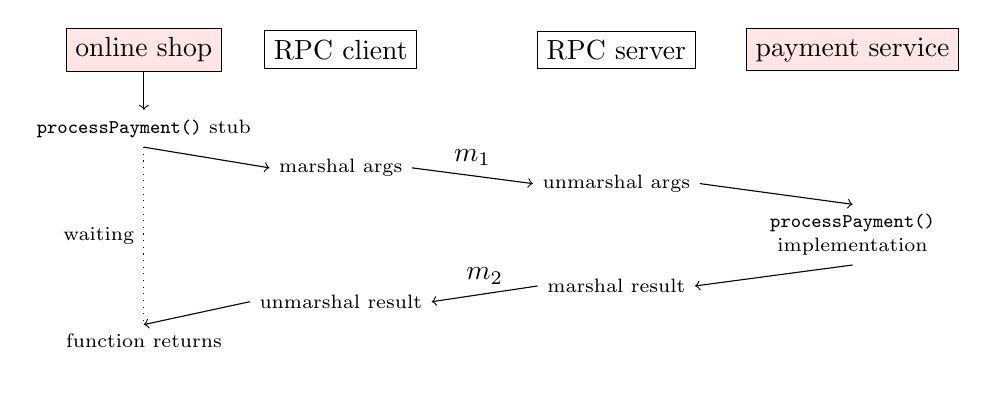
\begin{tikzpicture}
        \node [rectangle,fill=red!10,draw] (client) at (0,4) {online shop};
        \node [rectangle,draw] (rpc-client) at (2.5,4) {RPC client};
        \node [rectangle,draw] (rpc-server) at (6,4) {RPC server};
        \node [rectangle,fill=red!10,draw] (server) at (9,4) {payment service};
        \node [font=\scriptsize] (invoke) at (0,3) {\texttt{processPayment()} stub};
        \draw [->] (client) -- (invoke);
        \node<2-> [font=\scriptsize] (send-req) at (2.5,2.5) {marshal args};
        \draw<2-> [->] (invoke.south) -- (send-req.west);
        \node<2-> [font=\scriptsize] (recv-req) at (6,2.3) {unmarshal args};
        \draw<2-> [->] (send-req.east) -- node [above] {$m_1$} (recv-req.west);
        \node<3-> [font=\scriptsize] (exec) at (9,1.8) {\texttt{processPayment()}};
        \node<3-> [font=\scriptsize] (exec2) at (9,1.5) {implementation};
        \draw<3-> [->] (recv-req.east) -- (exec.north);
        \node<4-> [font=\scriptsize] (send-res) at (6,1) {marshal result};
        \draw<4-> [->] (exec2.south) -- (send-res.east);
        \node<4-> [font=\scriptsize] (recv-res) at (2.5,0.8) {unmarshal result};
        \draw<4-> [->] (send-res.west) -- node [above] {$m_2$} (recv-res.east);
        \node<5> [font=\scriptsize] (return) at (0,0.3) {function returns};
        \draw<5> [->] (recv-res.west) -- (return.north);
        \draw [dotted] (invoke.south) -- node [left,font=\scriptsize] {waiting} (0,0.5);
        \node at (0,0) {}; % so that messages below stay put as the slide builds
    \end{tikzpicture}
    \hspace*{-1cm}\mbox{
        \onslide<2->{
            $m_1$ = \begin{minipage}{5.5cm}
            \inputminted[fontsize=\scriptsize,frame=single,bgcolor=lightgrey]{json}{code/payment-rpc.json}
            \end{minipage}
        }
        \onslide<4->{
            $m_2$ = \begin{minipage}{3.8cm}
            \inputminted[fontsize=\scriptsize,frame=single,bgcolor=lightgrey]{json}{code/payment-response.json}
            \end{minipage}
        }
    }
\end{frame}
\inlineslide{s:payment-json}\label{l:payment-json}

The sending of the message from the RPC client to the RPC server may happen over HTTP (in which case this is also called a \emph{web service}), or one of a range of different network protocols may be used.
On the server side, the RPC framework unmarshals (decodes) the message and calls the desired function with the provided arguments.
When the function returns, the same happens in reverse: the function's return value is marshalled, sent as a message back to the client, unmarshalled by the client, and returned by the stub.
Thus, to the caller of the stub, it looks as if the function had executed locally.

\begin{frame}
    \label{s:rpc-problems}
    \frametitle{Remote Procedure Call (RPC)}
    Ideally, RPC makes a call to a remote function look the same as a local function call.\\[1em]
    \textbf{``Location transparency''}:\\ system hides where a resource is located.\\[1em]\pause
    In practice\dots
    \begin{itemize}
        \item what if the service crashes during the function call?
        \item what if a message is lost?
        \item what if a message is delayed?
        \item if something goes wrong, is it safe to retry?
    \end{itemize}
\end{frame}
\inlineslide{s:rpc-problems}

\supervision{
    Networks and nodes might fail.
    What are the implications for code that calls another node through RPC?
    How is RPC different from a local function call?
    Is location transparency achievable?
}{
    \begin{itemize}
        \item RPCs may time out if the request or response message is lost.
            Even if we retry, there is no guarantee that the messages will get through.
            The application must handle this error condition, and the possibility of failure may need to be reflected in the type signature.
            For example, Java RPC libraries often throw a checked exception, and JavaScript RPC clients often return a \emph{promise}, which can either succeed or fail.
        \item If a timeout occurs, the RPC client doesn't know whether the server executed the function; local function calls don't have this uncertainty.
        \item RPC is often much slower than a local function call, due to network latency.
            Moreover, network latency is often variable and unpredictable, while the execution speed of a local function is usually predictable.
        \item RPC clients and servers may need to take measures to make function invocation \emph{idempotent} (this concept is introduced in a later lecture), to allow safe retries in case of message loss.
        \item Another difference is that if an object reference is passed as an argument, a local function call can potentially mutate the object (unless it is immutable).
            This is not possible with RPC, since the remote function cannot access the caller's memory; the only way how the remote function can pass information back to the caller is through the return value, or through another RPC.
        \item Perfect location transparency can only be achieved by making local function calls more like RPCs (e.g.\ allowing them to unpredictably fail).
            This is undesirable in most cases, and therefore most systems do not attempt to completely hide the distinction between local and remote calls.
    \end{itemize}
}

Over the decades many variants of RPC have been developed, with the goal of making it easier to program distributed systems.
This includes object-oriented middleware such as CORBA in the 1990s.
However, the underlying distributed systems challenges have remained the same \citep{Waldo:1994wx}.

\begin{frame}
    \label{s:rpc-history}
    \frametitle{RPC history}
    \begin{itemize}
        \item SunRPC/ONC RPC (1980s, basis for NFS)
        \item CORBA: object-oriented middleware, hot in the 1990s
        \item Microsoft's DCOM and Java RMI (similar to CORBA)
        \item SOAP/XML-RPC: RPC using XML and HTTP (1998)
        \item Thrift (Facebook, 2007)
        \item gRPC (Google, 2015)
        \item REST (often with JSON)
        \item Ajax in web browsers
    \end{itemize}
\end{frame}
\inlineslide{s:rpc-history}

Today, the most common form of RPC is implemented using JSON data sent over HTTP.
A popular set of design principles for such HTTP-based APIs is known as \emph{representational state transfer} or \emph{REST} \citep{Fielding:2000}, and APIs that adhere to these principles are called \emph{RESTful}.
These principles include:
\begin{itemize}
    \item communication is stateless (each request is self-contained and independent from other requests),
    \item resources (objects that can be inspected and manipulated) are represented by URLs, and
    \item the state of a resource is updated by making a HTTP request with a standard method type, such as \texttt{POST} or \texttt{PUT}, to the appropriate URL.
\end{itemize}
The popularity of REST is due to the fact that JavaScript code running in a web browser can easily make this type of HTTP request, as shown in \autoref{l:javascript-rpc}.
In modern websites it is very common to use JavaScript to make HTTP requests to a server without reloading the whole page.
This technique is sometimes known as \emph{Ajax}.

\begin{frame}
    \label{s:javascript-rpc}
    \frametitle{RPC/REST in JavaScript}
    \inputminted{js}{code/payment-rpc.js}
\end{frame}
\inlineslide{s:javascript-rpc}\label{l:javascript-rpc}

The code on \autoref{l:javascript-rpc} takes the arguments \verb|args|, marshals them to JSON using \verb|JSON.stringify()|, and then sends them to the URL \verb|https://example.com/payments| using a HTTP POST request.
There are three possible outcomes: either the server returns a status code indicating success (in which case we unmarshal the response using \verb|response.json()|), or the server returns a status code indicating an error, or the request fails because no response was received from the server (most likely due to a network interruption).
The code calls either the \verb|success()| or the \verb|failure()| function in each of these cases.

Even though RESTful APIs and HTTP-based RPC originated on the web (where the client is JavaScript running in a web browser), they are now also commonly used with other types of client (e.g.\ mobile apps), or for server-to-server communication.

\begin{frame}
    \label{s:rpc-discussion}
    \frametitle{RPC in enterprise systems}
    \textbf{``Service-oriented architecture''} (SOA) / ``microservices'':\\[1em]
    splitting a large software application into multiple services\\ (on multiple nodes) that communicate via RPC.\\[1.5em]\pause

    Different services implemented in different languages:
    \begin{itemize}
        \item interoperability: datatype conversions
        \item \textbf{Interface Definition Language} (IDL): language-independent API specification
    \end{itemize}
\end{frame}
\inlineslide{s:rpc-discussion}

Such server-to-server RPC is especially common in large enterprises, whose software systems are too large and complex to run in a single process on a single machine.
To manage this complexity, the system is broken down into multiple services, which are developed and administered by different teams and which may even be implemented in different programming languages.
RPC frameworks facilitate the communication between these services.

When different programming languages are used, the RPC framework needs to convert datatypes such that the caller's arguments are understood by the code being called, and likewise for the function's return value.
A typical solution is to use an \emph{Interface Definition Language} (IDL) to provide language-independent type signatures of the functions that are being made available over RPC.
From the IDL, software developers can then automatically generate marshalling/unmarshalling code and RPC stubs for the respective programming languages of each service and its clients.
\autoref{l:rpc-idl} shows an example of the IDL used by gRPC, called \emph{Protocol Buffers}.
The details of the language are not important for this course.

\begin{frame}
    \label{s:rpc-idl}
    \frametitle{gRPC IDL example}
    \inputminted[fontsize=\scriptsize]{protobuf}{code/payment-rpc.proto}
\end{frame}
\inlineslide{s:rpc-idl}\label{l:rpc-idl}

% If the client sends the RPC request but receives no response, it doesn't know whether or not the server received and processed the request.
% It could resend the request if it doesn't hear back for a while, but that might cause the request to be performed more than once (e.g.\ charging a credit card twice), unless we take care to make the request idempotent.
% But even if we retry, there is no guarantee that the retried messages will get through either.
%
% Waiting forever is not a good approach, so in practice we have to give up after some timeout.
% As the client has not received a response, the RPC stub will not be able to return a value of the function's return type, but rather it will need to somehow indicate to the calling code that a timeout occurred, e.g.\ by throwing an exception.

\section{Models of distributed systems}\label{sec:system-models}

\begin{frame}
    \begin{center}
        Lecture 2\\[2em]
        \Large{\color{darkblue}{Models of distributed systems}}
    \end{center}
\end{frame}

A \emph{system model} captures our assumptions about how nodes and the network behave.
It is an abstract description of their properties, which can be implemented by various technologies in practice.
To illustrate common system models, we will start this section by looking at two classic thought experiments in distributed systems: the \emph{two generals problem} and the \emph{Byzantine generals problem}.

\subsection{The two generals problem}\label{sec:two-generals}

In the two generals problem \citep{Gray:1978}, we imagine two generals, each leading an army, who want to capture a city.
(Apologies for the militaristic analogy~-- I didn't come up with it!)
The city's defences are strong, and if only one of the two armies attacks, the army will be defeated.
However, if both armies attack at the same time, they will successfully capture the city.

\begin{frame}
    \label{s:two-generals}
    \frametitle{The two generals problem}
    \begin{center}
        \begin{tikzpicture}
            \node [rectangle,fill=red!10,draw] (army1) at (0,0) {army 1};
            \node [rectangle,fill=red!10,draw] (army2) at (8,0) {army 2};
            \node [circle,fill=blue!10,draw] (city) at (4,2) {city};
            \draw [thick,dashed,-{Stealth[length=3mm]}] (army1) -- node [left,yshift=0.2cm] {attack?} (city);
            \draw [thick,dashed,-{Stealth[length=3mm]}] (army2) -- node [right,yshift=0.2cm] {attack?} (city);
            \draw [doublebigarrow] (army1) -- node [below] {messengers} (army2);
        \end{tikzpicture}\\[1.5em]\pause
        \begin{tabular}{|c|c|c|}
            \hline
            army 1 & army 2 & outcome \\\hline
            does not attack & does not attack & nothing happens \\
            attacks & does not attack & army 1 defeated \\
            does not attack & attacks & army 2 defeated \\
            attacks & attacks & city captured \\\hline
        \end{tabular}\\[1.5em]
        \textbf{Desired:} army 1 attacks \emph{if and only if} army 2 attacks
    \end{center}
\end{frame}
\inlineslide{s:two-generals}\label{l:two-generals}

Thus, the two generals need to coordinate their attack plan.
This is made difficult by the fact that the two armies are camped some distance apart, and they can only communicate by messenger.
The messengers must pass through territory controlled by the city, and so they are sometimes captured.
Thus, a message sent by one general may or may not be received by the other general, and the sender does not know whether their message got through, except by receiving an explicit reply from the other party.
If a general does not receive any messages, it is impossible to tell whether this is because the other general didn't send any messages, or because all messengers were captured.

\begin{frame}
    \label{s:two-generals-comms}
    \frametitle{The two generals problem}
    \begin{center}
        \begin{tikzpicture}
            \node [rectangle,fill=red!10,draw] (gen1) at (0,3) {general 1};
            \node [rectangle,fill=red!10,draw] (gen2) at (8,3) {general 2};
            \draw (gen1) -- (0,0);
            \draw (gen2) -- (8,0);
            \draw [bigarrow] (0,2.2) -- node [above,sloped] {attack 10 Nov, okay?} (8,1.2);
            \draw [messageloss] (8,0.7) -- node [above,sloped] {10 Nov agreed!} (2,0);
        \end{tikzpicture}\pause\\[1em]
        From general 1's point of view, this is indistinguishable from:\\[1em]
        \begin{tikzpicture}
            \node [rectangle,fill=red!10,draw] (gen1) at (0,3) {general 1};
            \node [rectangle,fill=red!10,draw] (gen2) at (8,3) {general 2};
            \draw (gen1) -- (0,1);
            \draw (gen2) -- (8,1);
            \draw [messageloss] (0,2.2) -- node [above,sloped] {attack 10 Nov, okay?} (6,1.4);
        \end{tikzpicture}
    \end{center}
\end{frame}
\inlineslide{s:two-generals-comms}

What protocol should the two generals use to agree on a plan?
For each general there are two options: either the general promises to go ahead with the attack in any case (even if no response is received), or the general waits for an acknowledgement before committing to attack.
In the first case, the general who promises to go ahead risks being alone in the attack.
In the second case, the general who awaits acknowledgement shifts the problem to the other general, who must now decide whether to commit to attack (and risk being alone) or wait for an acknowledgement of the acknowledgement.

\begin{frame}
    \label{s:two-generals-proto}
    \frametitle{How should the generals decide?}
    \begin{enumerate}
        \item General 1 always attacks, even if no response is received?
            \begin{itemize}
                \item Send lots of messengers to increase probability that one will get through
                \item If all are captured, general 2 does not know about the attack, so general 1 loses\\[1em]\pause
            \end{itemize}
        \item General 1 only attacks if positive response from general 2 is received?
            \begin{itemize}
                \item Now general 1 is safe
                \item But general 2 knows that general 1 will only attack if general 2's response gets through
                \item Now general 2 is in the same situation as general 1 in option 1\\[0.5em]\pause
            \end{itemize}
    \end{enumerate}
    \textbf{No common knowledge}: the only way of knowing something is to communicate it
\end{frame}
\inlineslide{s:two-generals-proto}

The problem is that no matter how many messages are exchanged, neither general can ever be certain that the other army will also turn up at the same time.
A repeated sequence of back-and-forth acknowledgements can build up gradually increasing confidence that the generals are in agreement, but it can be proved that they cannot reach certainty by exchanging any finite number of messages.

This thought experiment demonstrates that in a distributed system, there is no way for one node to have certainty about the state of another node.
The only way how a node can know something is by having that knowledge communicated in a message.
On a philosophical note, this is perhaps similar to communication between humans: we have no telepathy, so the only way for someone else to know what you are thinking is by communicating it (through speech, writing, body language, etc).

As a practical example of the two generals problem, \autoref{l:two-generals-applied} adapts the model from \autoref{l:two-generals} to the application of paying for goods in an online shop.
The shop and the credit card payment processing service communicate per RPC, and some of these messages may be lost.
Nevertheless, the shop wants to ensure that it dispatches the goods only if they are paid for, and it only charges the customer card if the goods are dispatched.

\begin{frame}
    \label{s:two-generals-applied}
    \frametitle{The two generals problem applied}
    \begin{center}
        \begin{tikzpicture}
            \node [rectangle,fill=red!10,draw] (army1) at (0,0) {online shop};
            \node [rectangle,fill=red!10,draw] (army2) at (8,0) {payments service};
            \node [circle,fill=blue!10,draw] (city) at (4,2) {customer};
            \draw [thick,dashed,-{Stealth[length=3mm]}] (army1) -- node [left,yshift=0.2cm] {dispatch goods} (city);
            \draw [thick,dashed,-{Stealth[length=3mm]}] (army2) -- node [right,yshift=0.2cm] {charge credit card} (city);
            \draw [doublebigarrow] (army1) -- node [below] {RPC} (army2);
        \end{tikzpicture}\\[1.5em]\pause
        \begin{tabular}{|c|c|c|}
            \hline
            online shop & payments service & outcome \\\hline
            does not dispatch & does not charge & nothing happens \\
            dispatches & does not charge & shop loses money \\
            does not dispatch & charges & customer complaint \\
            dispatches & charges & everyone happy \\\hline
        \end{tabular}\\[1.5em]
        \textbf{Desired:} online shop dispatches \emph{if and only if} payment made
    \end{center}
\end{frame}
\inlineslide{s:two-generals-applied}\label{l:two-generals-applied}

In practice, the online shopping example does not exactly match the two generals problem: in this scenario, it is safe for the payments service to always go ahead with a payment, because if the shop ends up not being able to dispatch the goods, it can refund the payment.
The fact that a payment is something that can be undone (unlike an army being defeated) makes the problem solveable.
If the communication between shop and payment service is interrupted, the shop can wait until the connection is restored, and then query the payments service to find out the status of any transactions whose outcome was unknown.

\subsection{The Byzantine generals problem}\label{sec:byzantine}

The Byzantine generals problem \citep{Lamport:1982} has a similar setting to the two generals problem.
Again we have armies wanting to capture a city, though in this case there can be three or more.
Again generals communicate by messengers, although this time we assume that if a message is sent, it is always delivered correctly.

\begin{frame}
    \label{s:byzantine-generals}
    \frametitle{The Byzantine generals problem}
    \begin{center}
        \begin{tikzpicture}
            \node [rectangle,fill=red!10,draw] (army1) at (0,0) {army 1};
            \node [rectangle,fill=red!10,draw] (army2) at (8,0) {army 2};
            \node [rectangle,fill=red!10,draw] (army3) at (4,5.5) {army 3};
            \node [circle,fill=blue!10,draw] (city) at (4,2.5) {city};
            \draw [thick,dashed,-{Stealth[length=3mm]}] (army1) -- node [right,yshift=-0.2cm] {attack?} (city);
            \draw [thick,dashed,-{Stealth[length=3mm]}] (army2) -- node [left,yshift=-0.2cm] {attack?} (city);
            \draw [thick,dashed,-{Stealth[length=3mm]}] (army3) -- node [left,yshift=-0.4cm] {attack?} (city);
            \draw [doublebigarrow] (army1.east)  -- node [below] {messengers} (army2.west);
            \draw [doublebigarrow] (army1.north) -- node [left]  {messengers} (army3.south west);
            \draw [doublebigarrow] (army2.north) -- node [right] {messengers} (army3.south east);
        \end{tikzpicture}\\[1.5em]
        \textbf{Problem:} some of the generals might be traitors
    \end{center}
\end{frame}
\inlineslide{s:byzantine-generals}\label{l:byzantine-generals}

The challenge in the Byzantine setting is that some generals might be ``traitors'': that is, they might try to deliberately and maliciously mislead and confuse the other generals.
One example of such malicious behaviour is shown on \autoref{l:byzantine-generals-comms}: here, general 3 receives two contradictory messages from generals 1 and 2.
General 1 tells general 3 to attack, whereas general 2 claims that general 1 ordered a retreat.
It is impossible for general 3 to determine whether general 2 is lying (the first case), or whether general 2 is honest while general 1 is issuing contradictory orders (the second case).

\begin{frame}
    \label{s:byzantine-generals-comms}
    \frametitle{Generals that might lie}
    \begin{center}
        \begin{tikzpicture}
            \node [rectangle,fill=red!10,draw] (gen1) at (0,2.6) {general 1};
            \node [rectangle,fill=red!10,draw] (gen2) at (4.5,2.6) {general 2};
            \node [rectangle,fill=red!10,draw] (gen3) at (9,2.6) {general 3};
            \draw (gen1) -- (0,0);
            \draw (gen2) -- (4.5,0);
            \draw (gen3) -- (9,0);
            \draw [bigarrow] (0,2.0) -- node [above,sloped,pos=0.25] {attack!} (9,1.2);
            \draw [bigarrow] (0,1.3) -- node [above,sloped] {attack!} (4.5,0.9);
            \draw [bigarrow] (4.5,0.6) -- node [above,sloped] {general 1 said retreat!} (9,0.2);
        \end{tikzpicture}\pause\\[1em]
        From general 3's point of view, this is indistinguishable from:\\[1em]
        \begin{tikzpicture}
            \node [rectangle,fill=red!10,draw] (gen1) at (0,2.6) {general 1};
            \node [rectangle,fill=red!10,draw] (gen2) at (4.5,2.6) {general 2};
            \node [rectangle,fill=red!10,draw] (gen3) at (9,2.6) {general 3};
            \draw (gen1) -- (0,0);
            \draw (gen2) -- (4.5,0);
            \draw (gen3) -- (9,0);
            \draw [bigarrow] (0,2.0) -- node [above,sloped,pos=0.25] {attack!} (9,1.2);
            \draw [bigarrow] (0,1.3) -- node [above,sloped] {retreat!} (4.5,0.9);
            \draw [bigarrow] (4.5,0.6) -- node [above,sloped] {general 1 said retreat!} (9,0.2);
        \end{tikzpicture}
    \end{center}
\end{frame}
\inlineslide{s:byzantine-generals-comms}\label{l:byzantine-generals-comms}

The honest generals don't know who the malicious generals are, but the malicious generals may collude and secretly coordinate their actions.
We might even assume that all of the malicious generals are controlled by an evil adversary.
The Byzantine generals problem is then to ensure that all honest generals agree on the same plan (e.g.\ whether to attack or to retreat).
It is impossible to specify what the malicious generals are going to do, so the best we can manage is to get the honest generals to agree.

This is difficult: in fact, it can be proved that some variants of the problem can be solved only if strictly fewer than one third of the generals are malicious.
That is, in a system with $3f+1$ generals, no more than $f$ may be malicious.
For example, a system with 4 generals can tolerate $f=1$ malicious general, and a system with 7 generals can tolerate $f=2$.

\begin{frame}
    \label{s:byzantine-discussion}
    \frametitle{The Byzantine generals problem}
    \begin{itemize}
        \item Up to $f$ generals might behave malicously\\[0.5em]
        \item Honest generals don't know who the malicious ones are\\[0.5em]
        \item The malicious generals may collude\\[0.5em]
        \item Nevertheless, honest generals must agree on plan\\[2em]\pause
        \item Theorem: need $3f+1$ generals in total to tolerate $f$ malicious generals (i.e.\ $< \frac{1}{3}$ may be malicious)\\[0.5em]
        \item Cryptography (digital signatures) helps~-- but problem remains hard\\[0.5em]
    \end{itemize}
\end{frame}
\inlineslide{s:byzantine-discussion}

The problem is made somewhat easier if generals use cryptography (\emph{digital signatures}) to prove who said what: for example, this would allow general 2 to prove to general 3 what general 1's order was, and thus demonstrate general 2's honesty.
We will not go into details of digital signatures in this course, as they are covered in the Security course (\whenissecurity).
However, even with signatures, the Byzantine generals problem remains challenging.

Is the Byzantine generals problem of practical relevance?
Real distributed systems do often involve complex trust relationships.
For example, a customer needs to trust an online shop to actually deliver the goods they ordered, although they can dispute the payment via their bank if the goods never arrive or if they get charged too much.
But if an online shop somehow allowed customers to order goods without paying for them, this weakness would no doubt be exploited by fraudsters, so the shop must assume that customers are potentially malicious.
On the other hand, for RPC between services belonging to the shop, running in the same datacentre, one service can probably trust the other services run by the same company.
The payments service doesn't fully trust the shop, since someone might set up a fraudulent shop or use stolen credit card numbers, but the shop probably does trust the payments service.
And so on.
And in the end, we want the customer, the online shop, and the payments service to agree on any order that is placed.
The Byzantine generals problem is a simplification of such complex trust relationships, but it is a good starting point for studying systems in which some participants might behave maliciously.

\begin{frame}
    \label{s:byzantine-payment}
    \frametitle{Trust relationships and malicious behaviour}
    \begin{center}
        \begin{tikzpicture}
            \node [rectangle,fill=red!10,draw] (army1) at (0,0) {online shop};
            \node [rectangle,fill=red!10,draw] (army2) at (8,0) {payments service};
            \node [rectangle,fill=red!10,draw] (army3) at (4,5.5) {customer};
            \node [circle,fill=blue!10,draw] (city) at (4,2.5) {order};
            \draw [thick,dashed,-{Stealth[length=3mm]}] (army1) -- node [right,yshift=-0.2cm] {agree?} (city);
            \draw [thick,dashed,-{Stealth[length=3mm]}] (army2) -- node [left,yshift=-0.2cm] {agree?} (city);
            \draw [thick,dashed,-{Stealth[length=3mm]}] (army3) -- node [left,yshift=-0.4cm] {agree?} (city);
            \draw [doublebigarrow] (army1.east)  -- node [below] {RPC} (army2.west);
            \draw [doublebigarrow] (army1.north) -- node [left]  {RPC} (army3.south west);
            \draw [doublebigarrow] (army2.north) -- node [right] {RPC} (army3.south east);
        \end{tikzpicture}\\[1.5em]
        Who can trust whom?
    \end{center}
\end{frame}
\inlineslide{s:byzantine-payment}\label{l:byzantine-payment}

Before we move on, a brief digression about the origin of the word ``Byzantine''.
The term comes from the Byzantine empire, named after its capital city Byzantium or Constantinople, which is now Istanbul in Turkey.
There is no historical evidence that the generals of the Byzantine empire were any more prone to intrigue and conspiracy than those elsewhere.
Rather, the word \emph{Byzantine} had been used in the sense of ``excessively complicated, bureaucratic, devious'' long before Leslie Lamport adopted the word to describe the Byzantine generals problem; the exact etymology is unclear.

\pagebreak[3]
\begin{frame}
    \label{s:byzantine-empire}
    \frametitle{The Byzantine empire (650 CE)}
    \begin{tikzpicture}
        \node at (0,0) {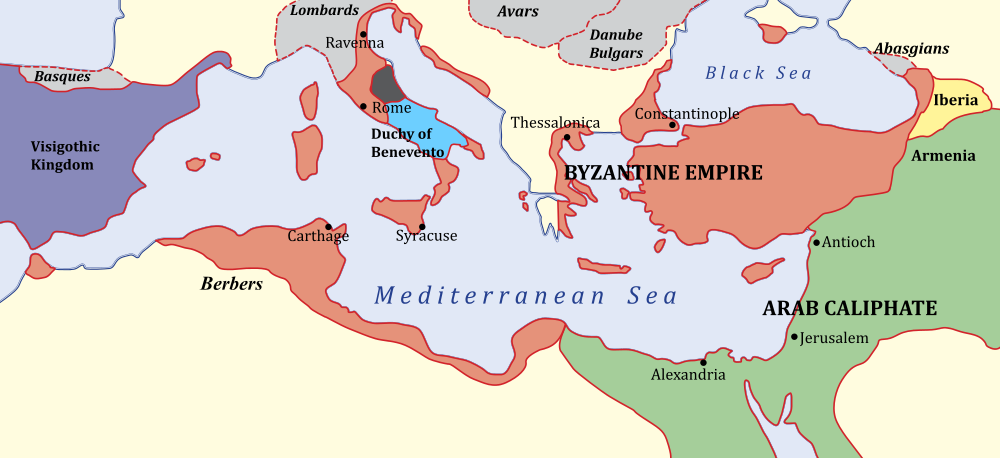
\includegraphics[height=5cm]{images/byzantium650.png}};
        \node (byzantium) at (2.4,3) {Byzantium/Constantinople/Istanbul};
        \draw [-Stealth,line width=4pt] (byzantium) -- (1.9,1.2);
    \end{tikzpicture}
    {\scriptsize Source: \url{https://commons.wikimedia.org/wiki/File:Byzantiumby650AD.svg}}\\[1em]
    \textbf{``Byzantine''} has long been used for ``excessively complicated, bureaucratic, devious'' (e.g.\ \emph{``the Byzantine tax law''})
\end{frame}
\inlineslide{s:byzantine-empire}\label{l:byzantine-empire}

\subsection{Describing nodes and network behaviour}\label{sec:system-behaviour}

When designing a distributed algorithm, a \emph{system model} is how we specify our assumptions about what faults may occur.

\begin{frame}
    \label{s:system-model}
    \frametitle{System models}
    We have seen two thought experiments:
    \begin{itemize}
        \item Two generals problem: a model of networks
        \item Byzantine generals problem: a model of node behaviour
    \end{itemize}
    In real systems, both nodes and networks may be faulty!\\[2em]\pause
    Capture assumptions in a \textbf{system model} consisting of:
    \begin{itemize}
        \item Network behaviour (e.g.\ message loss)
        \item Node behaviour (e.g.\ crashes)
        \item Timing behaviour (e.g.\ latency)
    \end{itemize}
    Choice of models for each of these parts.
\end{frame}
\inlineslide{s:system-model}\label{l:system-model}

\begin{frame}
    \label{s:shark-bite}
    \frametitle{Networks are unreliable}
    % Source for network-cable.jpg: https://pixabay.com/photos/modem-antenna-wire-cable-router-5436144/
    % (Royalty-free, no attribution required)
    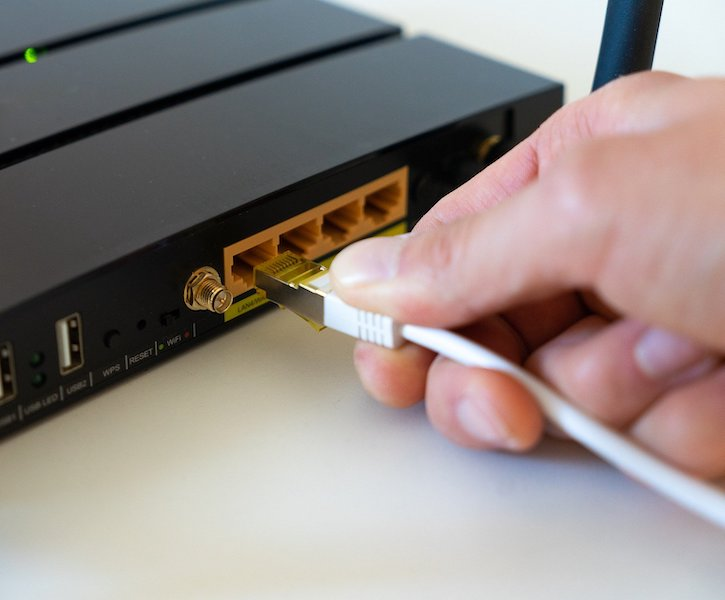
\includegraphics[height=4cm]{images/network-cable.jpg}
    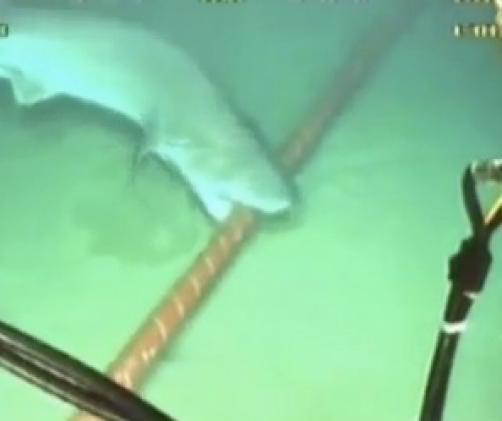
\includegraphics[height=4cm]{images/shark-bite.jpg}\\[1em]
    In the sea, sharks bite fibre optic cables \\
    {\scriptsize\url{https://slate.com/technology/2014/08/shark-attacks-threaten-google-s-undersea-internet-cables-video.html}}\\[1em]
    On land, cows step on the cables \\
    {\scriptsize\url{https://twitter.com/uhoelzle/status/1263333283107991558}}
\end{frame}
\inlineslide{s:shark-bite}\label{l:shark-bite}

Let's start with the network.
No network is perfectly reliable: even in carefully engineered systems with redundant network links, things can go wrong \citep{Bailis:2014jx}.
Someone might accidentally unplug the wrong network cable.
Sharks and cows have both been shown to cause damage and interruption to long-distance networks (see links on \autoref{l:shark-bite}).
Or a network may be temporarily overloaded, perhaps by accident or perhaps due to a denial-of-service attack.
Any of these can cause messages to be lost.

In a system model, we take a more abstract view, which saves us from the details of worrying about sharks and cows.
Most distributed algorithms assume that the network provides bidirectional message-passing between a pair of nodes, also known as \emph{point-to-point} or \emph{unicast} communication.
Real networks do sometimes allow \emph{broadcast} or \emph{multicast} communication (sending a packet to many recipients at the same time, which is used e.g.\ for discovering a printer on a local network), but broadly speaking, assuming unicast-only is a good model of the Internet today.
Later, in \autoref{sec:broadcast}, we will show how to implement broadcast on top of unicast communication.

We can then choose how reliable we want to assume these links to be.
Most algorithms assume one of the three choices listed on \autoref{l:model-network}.

\begin{frame}
    \label{s:model-network}
    \frametitle{System model: network behaviour}
    Assume bidirectional \textbf{point-to-point} communication between two nodes, with one of:\pause
    \begin{itemize}
        \item \textbf{Reliable} (perfect) links:\\
            A message is received if and only if it is sent.\tikz[remember picture]\node (reliable) {};\\
            Messages may be reordered.\pause
        \item \textbf{Fair-loss} links:\\
            Messages may be lost, duplicated, or reordered.\tikz[remember picture]\node (fairloss) {};\\
            If you keep retrying, a message eventually gets through.\pause
        \item \textbf{Arbitrary} links (active adversary):\\
            A malicious adversary may interfere with messages\tikz[remember picture]\node (arbitrary) {};\\
            (eavesdrop, modify, drop, spoof, replay).\\[1em]
    \end{itemize}\pause
    \textbf{Network partition}: some links dropping/delaying all messages for extended period of time
    \begin{tikzpicture}[remember picture,overlay]
        \draw<6-> [-Stealth,red,line width=4pt] (fairloss.north) .. controls +(1.6,0) and +(1.6,0) ..
            node [right,red,align=left] {retry +\\dedup} (reliable);
        \draw<7> [-Stealth,red,line width=4pt] (arbitrary) .. controls +(1.6,0) and +(1.6,0) ..
            node [right,red,align=left] {TLS} (fairloss.south);
    \end{tikzpicture}
\end{frame}
\inlineslide{s:model-network}\label{l:model-network}

Interestingly, it is possible to convert some types of link into others.
For example, if we have a fair-loss link, we can turn it into a reliable link by continually retransmitting lost messages until they are finally received, and by filtering out duplicated messages on the recipient side.
The fair-loss assumption means that any \emph{network partition} (network interruption) will last only for a finite period of time, but not forever, so we can guarantee that every message will eventually be received.

Of course, any messages sent during a network partition will only be received after the interruption is repaired, which may take a long time, but the definitions on \autoref{l:model-network} do not say anything about network delay or latency.
We will get to that topic on \autoref{l:model-synchrony}.

The TCP protocol, which we discussed briefly in \autoref{sec:web}, performs this kind of retry and deduplication at the network packet level.
However, TCP is usually configured with a timeout, so it will give up and stop retrying after a certain time, typically on the order of one minute.
To overcome network partitions that last for longer than this duration, a separate retry and deduplication mechanism needs to be implemented in addition to that provided by TCP.

An arbitrary link is an accurate model for communication over the Internet: whenever your communication is routed through a network (be it a coffee shop wifi or an Internet backbone network), the operator of that network can potentially interfere with and manipulate your network packets in arbitrary ways.
Someone who manipulates network traffic is also known as an \emph{active adversary}.
Fortunately, it is \emph{almost} possible to turn an arbitrary link into a fair-loss link using cryptographic techniques.
The \emph{Transport Layer Security} (TLS) protocol, which provides the ``s'' for ``secure'' in \verb|https://|, prevents an active adversary from eavesdropping, modifying, spoofing, or replaying traffic (more on this in the Security course, \whenissecurity).

The only thing that TLS cannot prevent is the adversary dropping (blocking) communication.
Thus, an arbitrary link can be converted into a fair-loss link only if we assume that the adversary does not block communication forever.
In some networks, it might be possible to route around the interrupted network link, but this is not always the case.

Thus, the assumption of a reliable network link is perhaps not as unrealistic as it may seem at first glance: generally it is possible for all sent messages to be received, as long as we are willing to wait for a potentially arbitrary period of time for retries during a network partition.
However, we also have to consider the possibility that the sender of a message may crash while attempting to retransmit a message, which may cause that message to be permanently lost.
This brings us to the topic of node crashes.

\begin{frame}
    \label{s:model-nodes}
    \frametitle{System model: node behaviour}
    Each node executes a specified algorithm,\\assuming one of the following:
    \begin{itemize}
        \item \textbf{Crash-stop} (fail-stop):\\
            A node is faulty if it crashes (at any moment).\\
            After crashing, it stops executing forever.\pause
        \item \textbf{Crash-recovery} (fail-recovery):\\
            A node may crash at any moment, losing its in-memory state.
            It may resume executing sometime later.\pause
        \item \textbf{Byzantine} (fail-arbitrary):\\
            A node is faulty if it deviates from the algorithm.\\
            Faulty nodes may do anything, including crashing or malicious behaviour.\\[1em]
    \end{itemize}
    A node that is not faulty is called \textbf{``correct''}
\end{frame}
\inlineslide{s:model-nodes}\label{l:model-nodes}

In the \emph{crash-stop} model, we assume that after a node crashes, it never recovers.
This is a reasonable model for an unrecoverable hardware fault, or for the situation where a person drops their phone in the toilet, after which it is permanently out of order.
With a software crash, the crash-stop model might seem unrealistic, because we can just restart the node, after which it will recover.
Nevertheless, some algorithms assume a crash-stop model, since that makes the algorithm simpler.
In this case, a node that crashes and recovers would have to re-join the system as a new node.
Alternatively, the \emph{crash-recovery} model explicitly allows nodes to restart and resume processing after a crash.

Finally, the \emph{Byzantine} model is the most general model of node behaviour: as in the Byzantine generals problem, a faulty node may not only crash, but also deviate from the specified algorithm in arbitrary ways, including exhibiting malicious behaviour.
A bug in the implementation of a node could also be classed as a Byzantine fault.
However, if all of the nodes are running the same software, they will all have the same bug, and so any algorithm that is predicated on less than one third of nodes being Byzantine-faulty will not be able to tolerate such a bug.
In principle, we could try using several different implementations of the same algorithm, but this is rarely a practical option.

In the case of the network, it was possible to convert one model to another using generic protocols.
This is not the case with the different models of node behaviour.
For instance, an algorithm designed for a crash-recovery system model may look very different from a Byzantine algorithm.

\begin{frame}
    \label{s:model-synchrony}
    \frametitle{System model: synchrony (timing) assumptions}
    Assume one of the following for network and nodes:
    \begin{itemize}
        \item \textbf{Synchronous}:\\
            Message latency no greater than a known upper bound.\\
            Nodes execute algorithm at a known speed.\pause
        \item \textbf{Partically synchronous}:\\
            The system is asynchronous for some finite (but unknown) periods of time, synchronous otherwise.\pause
        \item \textbf{Asynchronous}:\\
            Messages can be delayed arbitrarily.\\
            Nodes can pause execution arbitrarily.\\
            No timing guarantees at all.\\[1em]
    \end{itemize}
    \textbf{Note}: other parts of computer science use the terms ``synchronous'' and ``asynchronous'' differently.
\end{frame}
\inlineslide{s:model-synchrony}\label{l:model-synchrony}

The third part of a system model is the synchrony assumption, which is about timing.
The three choices we can make here are \emph{synchronous}, \emph{asynchronous}, or \emph{partially synchronous} \citep{Dwork:1988dr}.
(Note that the definitions of these terms differ somewhat across different parts of computer science; our definitions here are standard in the field of distributed computing.)

A synchronous system is what we would love to have: a message sent over the network never takes longer than some known maximum latency, and nodes always execute their algorithm at a predictable speed.
Many problems in distributed computing are much easier if you assume a synchronous system.
And it is tempting to assume synchrony, because networks and nodes are well-behaved \emph{most of the time}, and so this assumption is often true.

Unfortunately, \emph{most of the time} is not the same as \emph{always}, and algorithms designed for a synchronous model often fail catastrophically if the assumptions of bounded latency and bounded execution speed are violated, even just for a short while, and even if this happens rarely.
And in practical systems, there are many reasons why network latency or execution speed may sometimes vary wildly, see \autoref{l:timing-violations}.

The other extreme is an asynchronous model, in which we make no timing assumptions at all: we allow messages to be delayed arbitrarily in the network, and we allow arbitrary differences in nodes' processing speeds (for example, we allow one node to pause execution while other nodes continue running normally).
Algorithms that are designed for an asynchronous model are typically very robust, because they are unaffected by any temporary network interruptions or spikes in latency.

Unfortunately, some problems in distributed computing are impossible to solve in an asynchronous model, and therefore we have the \emph{partially synchronous} model as a compromise.
In this model, we assume that our system is synchronous and well-behaved most of the time, but occasionally it may flip into asynchronous mode in which all timing guarantees are off, and this can happen unpredictably.
The partially synchronous model is good for many practical systems, but using it correctly requires care.

\begin{frame}
    \label{s:timing-violations}
    \frametitle{Violations of synchrony in practice}
    Networks usually have quite predictable latency, which can occasionally increase:
    \begin{itemize}
        \item Message loss requiring retry
        \item Congestion/contention causing queueing
        \item Network/route reconfiguration\\[1em]
    \end{itemize}\pause
    Nodes usually execute code at a predictable speed, with occasional pauses:
    \begin{itemize}
        \item Operating system scheduling issues, e.g.\ priority inversion
        \item Stop-the-world garbage collection pauses
        \item Page faults, swap, thrashing
    \end{itemize}
    Real-time operating systems (RTOS) provide scheduling guarantees, but most distributed systems do not use RTOS
\end{frame}
\inlineslide{s:timing-violations}\label{l:timing-violations}

There are many reasons why a system may violate synchrony assumptions.
We have already talked about latency increasing without bound if messages are lost and retransmitted, especially if we have to wait for a network partition to be repaired before the messages can get through.
Another reason for latency increases in a network is congestion resulting in queueing of packets in switch buffers.
Network reconfiguration can also cause large delays: even within a single datacenter, there have been documented cases of packets being delayed for more than a minute \citep{Imbriaco:2012tx}.

We might expect that the speed at which nodes execute their algorithms is constant: after all, an instruction generally takes a fixed number of CPU clock cycles, and the clock speed doesn't vary much.
However, even on a single node, there are many reasons why a running program may unexpectedly get paused for significant amounts of time.
Scheduling in the operating system can preempt a running thread and leave it paused while other programs run, especially on a machine under heavy load.
A real problem in memory-managed languages such as Java is that when the garbage collector runs, it needs to pause all running threads from time to time (this is known as a \emph{stop-the-world} garbage collection pause).
On large heaps, such pauses can be as long as several minutes \citep{Thompson:2013}!
Page faults are another reason why a thread may get suspended, especially when there is not much free memory left.

As you know from the concurrent systems half of this course, threads can and will get preempted even at the most inconvenient moments, anywhere in a program.
In a distributed system, this is particularly problematic, because for one node, time appears to ``stand still'' while it is paused, and during this time all other nodes continue executing their algorithms normally.
Other nodes may even notice that the paused node is not responding, and assume that it has crashed.
After a while, the paused node resumes processing, without even realising that it was paused for a significant period of time.

Combined with the many reasons for variable network latency, this means that in practical systems, it is very rarely safe to assume a synchronous system model.
Most distributed algorithms need to be designed for the asynchronous or partially synchronous model.

\begin{frame}
    \label{s:model-summary}
    \frametitle{System models summary}
    For each of the three parts, pick one:\\
    \begin{itemize}
        \item \textbf{Network:}\\
            reliable, fair-loss, or arbitrary\\[1em]
        \item \textbf{Nodes:}\\
            crash-stop, crash-recovery, or Byzantine\\[1em]
        \item \textbf{Timing:}\\
            synchronous, partially synchronous, or asynchronous\\[1em]
    \end{itemize}
    This is the basis for any distributed algorithm.\\
    If your assumptions are wrong, all bets are off!
\end{frame}
\inlineslide{s:model-summary}\label{l:model-summary}

\subsection{Fault tolerance and high availability}\label{sec:fault-tolerance}

As highlighted in \autoref{sec:pros-cons}, one reason for building distributed systems is to achieve higher reliability than is possible with a single computer.
We will now explore this idea further in the light of the system models we have discussed.

From a business point of view, what usually matters most is the \emph{availability} of a service, such as a website.
For example, an online shop wants to be able to sell products at any time of day or night: any outage of the website means a lost opportunity to make money.
For other services, there may even be contractual agreements with customers requiring the service to be available.
If a service is unavailable, this can also damage the reputation of the service provider.

The availability of a service is typically measured in terms of its ability to respond correctly to requests within a certain time.
The definition of whether a service is ``available'' or ``unavailable'' can be somewhat arbitrary: for example, if it takes 5 seconds to load a page, do we still consider that website to be available?
What if it takes 30 seconds?
An hour?

\begin{frame}
    \label{s:availability}
    \frametitle{Availability}
    Online shop wants to sell stuff 24/7! \\
    Service unavailability = downtime = losing money \\[1em]
    Availability = uptime = fraction of time that a service is functioning correctly
    \begin{itemize}
        \item ``Two nines'' = 99\% up = down 3.7 days/year
        \item ``Three nines'' = 99.9\% up = down 8.8 hours/year
        \item ``Four nines'' = 99.99\% up = down 53 minutes/year
        \item ``Five nines'' = 99.999\% up = down 5.3 minutes/year\\[1.5em]
    \end{itemize}\pause
    \textbf{Service-Level Objective} (SLO):\\ e.g. ``99.9\% of requests in a day get a response in 200~ms''\\[1em]
    \textbf{Service-Level Agreement} (SLA):\\ contract specifying some SLO, penalties for violation
\end{frame}
\inlineslide{s:availability}\label{l:availability}

Typically, the availability expectations of a service are formalised as a \emph{service-level objective} (SLO), which typically specifies the percentage of requests that need to return a correct response within a specified timeout, as measured by a certain client over a certain period of time.
A \emph{service-level agreement} (SLA) is a contract that specifies some SLO, as well as the consequences if the SLO is not met (for example, the service provider may need to offer a refund to its customers).

Faults (such as node crashes or network interruptions) are a common cause of unavailability.
In order to increase availability, we can reduce the frequency of faults, or we can design systems to continue working despite some of its components being faulty; the latter approach is called \emph{fault tolerance}.
Reducing the frequency of faults is possible through buying higher-quality hardware and introducing redundancy, but this approach can never reduce the probability of faults to zero.
Instead, fault tolerance is the approach taken by many distributed systems.

\begin{frame}
    \label{s:fault-tolerance}
    \frametitle{Achieving high availability: fault tolerance}
    \textbf{Failure}: system as a whole isn't working\\[1em]
    \textbf{Fault}: some part of the system isn't working
    \begin{itemize}
        \item Node fault: crash (crash-stop/crash-recovery),\\deviating from algorithm (Byzantine)
        \item Network fault: dropping or significantly delaying messages\\[1em]
    \end{itemize}
    \textbf{Fault tolerance}:\\system as a whole continues working, despite faults\\
    (some maximum number of faults assumed)\\[1em]
    \textbf{Single point of failure} (SPOF):\\ node/network link whose fault leads to failure
\end{frame}
\inlineslide{s:fault-tolerance}\label{l:fault-tolerance}

If all nodes crash and don't recover, then no algorithm will be able to get any work done, so it does not make sense to tolerate arbitrary numbers of faults.
Rather, an algorithm is designed to tolerate some specified number of faults: for example, some distributed algorithms are able to make progress provided that fewer than half of the nodes have crashed.

In fault-tolerant systems we want to avoid \emph{single points of failure} (SPOF), i.e.\ components that would cause an outage if they were to become faulty.
For example, the Internet is designed to have no SPOF: there is no one server or router whose destruction would bring down the entire Internet (although the loss of some components, such as key intercontinental fibre links, does cause noticeable disruption).
% Also BGP hijacking...

The first step towards tolerating faults is to detect faults, which is often done with a \emph{failure detector}.
(``Fault detector'' would be more logical, but ``failure detector'' is the conventional term.)
A failure detector usually detects crash faults.
Byzantine faults are not always detectable, although in some cases Byzantine behaviour does leave evidence that can be used to identify and exclude malicious nodes.

\begin{frame}
    \label{s:failure-detector}
    \frametitle{Failure detectors}
    \textbf{Failure detector}:\\algorithm that detects whether another node is faulty\\[1em]
    \textbf{Perfect failure detector}:\\labels a node as faulty if and only if it has crashed\\[1em]\pause
    \textbf{Typical implementation} for crash-stop/crash-recovery:\\
    send message, await response, label node as crashed if no reply within some timeout\\[1em]\pause
    \textbf{Problem}:\\cannot tell the difference between crashed node, temporarily
    unresponsive node, lost message, and delayed message\\[1em]
\end{frame}
\inlineslide{s:failure-detector}\label{l:failure-detector}

In most cases, a failure detector works by periodically sending messages to other nodes, and labelling a node as crashed if no response is received within the expected time.
Ideally, we would like a timeout to occur if and only if the node really has crashed (this is called a \emph{perfect failure detector}).
However, the two generals problem tells us that this is not a totally accurate way of detecting a crash, because the absence of a response could also be due to message loss or delay.

A perfect timeout-based failure detector exists only in a synchronous crash-stop system with reliable links; in a partially synchronous system, a perfect failure detector does not exist.
Moreover, in an asynchronous system, no timeout-based failure exists, since timeouts are meaningless in the asynchronous model.
However, there is a useful failure detector that exists in partially synchronous systems: the \emph{eventually perfect failure detector} \citep{Chandra:1996}.

\begin{frame}
    \label{s:eventual-detector}
    \frametitle{Failure detection in partially synchronous systems}
    Perfect timeout-based failure detector exists only in a synchronous crash-stop system with reliable links.\\[1em]
    \textbf{Eventually perfect failure detector}:
    \begin{itemize}
        \item May \emph{temporarily} label a node as crashed,\\ even though it is correct
        \item May \emph{temporarily} label a node as correct,\\ even though it has crashed
        \item But \emph{eventually}, labels a node as crashed\\ if and only if it has crashed\\[1em]
    \end{itemize}
    Reflects fact that detection is not instantaneous, and we may have spurious timeouts
\end{frame}
\inlineslide{s:eventual-detector}\label{l:eventual-detector}

We will see later how to use such a failure detector to design fault-tolerance mechanisms and to automatically recover from node crashes.
Using such algorithms it is possible to build systems that are highly available.
Tolerating crashes also makes day-to-day operations easier: for example, if a service can tolerate one out of three nodes being unavailable, then a software upgrade can be rolled out by installing it and restarting one node at a time, while the remaining two nodes continue running the service.
Being able to roll out software upgrades in this way, without clients noticing any interruption, is important for many organisations that are continually working on their software.

%\begin{frame}
    %\label{s:availability-discuss}
    %\frametitle{High availability costs and benefits}
    % TODO: visualise a rolling software upgrade?
%\end{frame}
%\inlineslide{s:availability-discuss}\label{l:availability-discuss}

For safety-critical applications, such as air-traffic control systems, it is undoubtedly important to invest in good fault-tolerance mechanisms.
However, it is not the case that higher availability is always better.
Reaching extremely high availability requires a highly focussed engineering effort, and often conservative design choices.
For example, the old-fashioned fixed-line telephone network is designed for ``five nines'' availability, but the downside of this focus on availability is that it has been very slow to evolve.
Most Internet services do not even reach four nines because of diminishing returns: beyond some point, the additional cost of achieving higher availability exceeds the cost of occasional downtime, so it is economically rational to accept a certain amount of downtime.

\supervision{\label{q:fifo-links}
    Reliable network links allow messages to be reordered.
    Give pseudocode for an algorithm that strengthens the properties of a reliable point-to-point link such that messages are received in the order they were sent (this is called a FIFO link), assuming an asynchronous crash-stop system model.
}{
    The sender attaches a sequence number to each message, and increments that number for each message sent.
    The recipient delivers messages in increasing order by sequence number.
    This may require buffering a message on the recipient side until messages with prior sequence numbers have arrived.

    \begin{algorithmic}
        \On{initialisation}
            \State [We have a separate copy of the following variables for each network link.]
            \State $\mathit{lastSent} := 0;\; \mathit{nextReceived} := 1;\; \mathit{buffer} := \{\}$
        \EndOn
        \State
        \On{request to send message $m$ over FIFO link}
            \State \textit{lastSent}++
            \State send $(m, \mathit{lastSent})$ via the underlying network link
        \EndOn
        \State
        \On{receiving $(m, n)$ via the underlying network link}
            \State $\mathit{buffer} := \mathit{buffer} \cup \{(m,n)\}$
            \While{$\exists m'.\; (m', \mathit{nextReceived}) \in \mathit{buffer}$}
                \State deliver $m'$ to the application
                \State \textit{nextReceived}++
            \EndWhile
        \EndOn
    \end{algorithmic}
}

\supervision{
    How do we need to change the algorithm from \autoref{q:fifo-links} if we assume a crash-recovery model instead of a crash-stop model?
}{
    When a node crashes and recovers, all of its in-memory state is lost.
    The sequence number algorithm maintains state in the form of the variables \textit{lastSent}, \textit{nextReceived}, and \textit{buffer}.
    This information needs to be preserved across crashes, so it must be maintained in non-volatile storage (e.g.\ on disk).

    Another issue is that a node may crash while in the process of sending or delivering a message.
    In that case, we will need to decide: does that message get sent/delivered after recovering from the crash?
    If so, the information about such in-progress operations will also need to be written to non-volatile storage.
}

\newpage
\section{Time, clocks, and ordering of events}\label{sec:time}

\begin{frame}
    \begin{center}
        Lecture 3\\[2em]
        \Large{\color{darkblue}{Time, clocks, and ordering of events}}
    \end{center}
\end{frame}

Let's start with a riddle, which will be resolved later in this lecture.

\begin{frame}
    \label{s:mystery}
    \frametitle{A detective story}
    In the night from 30 June to 1 July 2012 (UK time), many online services and systems around the world crashed simultaneously.\\[1em]
    Servers locked up and stopped responding.\\[1em]
    Some airlines could not process any reservations or check-ins for several hours.\\[1em]
    What happened?
\end{frame}
\inlineslide{s:mystery}\label{l:mystery}

In this lecure we will look at the concept of time in distributed systems.
We have already seen that our assumptions about timing form a key part of the system model that distributed algorithms rely on.
For example, timeout-based failure detectors need to measure time to determine when a timeout has elapsed.
Operating systems rely extensively on timers and time measurements in order to schedule tasks, keep track of CPU usage, and many other purposes.
Applications often want to record the time and date at which events occurred: for example, when debugging an error in a distributed system, timestamps are helpful for debugging, since they allow us to reconstruct which things happened around the same time on different nodes.
All of these require more or less accurate measurements of time.

\begin{frame}
    \label{s:clocks-intro}
    \frametitle{Clocks and time in distributed systems}
    Distributed systems often need to measure time, e.g.:
    \begin{itemize}
        \item Schedulers, timeouts, failure detectors, retry timers\pause
        \item Performance measurements, statistics, profiling\pause
        \item Log files \& databases: record when an event occurred\pause
        \item Data with time-limited validity (e.g.\ cache entries)\pause
        \item Determining order of events across several nodes\\[1em]\pause
    \end{itemize}
    We distinguish two types of clock:
    \begin{itemize}
        \item \textbf{physical clocks}: count number of seconds elapsed
        \item \textbf{logical clocks}: count events, e.g.\ messages sent\\[1em]
    \end{itemize}\pause
    \textbf{NB.} Clock in digital electronics (oscillator)\\$\neq$ clock in distributed systems (source of \textbf{timestamps})
\end{frame}
\inlineslide{s:clocks-intro}\label{l:clocks-intro}

% Demo: load www.cst.cam.ac.uk in browser, open developer tools and view certificate expiry date
% Also run `dig www.cst.cam.ac.uk` in a terminal and see how the TTL counts down

\subsection{Physical clocks}\label{sec:physical-clocks}

We will start by discussing \emph{physical clocks}, which are the types of clocks you are familiar with from everyday usage.
Physical clocks include analog/mechanical clocks based on pendulums or similar mechanisms, and digital clocks based e.g.\ on a vibrating quartz crystal.
Quartz clocks are found in most wristwatches, in every computer and mobile phone, in microwave ovens that display the time, and many other everyday objects.

\begin{frame}
    \label{s:quartz-clocks}
    \frametitle{Quartz clocks}
    \begin{columns}
        \begin{column}{0.5\textwidth}
            \begin{itemize}
                \item Quartz crystal laser-trimmed to mechanically resonate at a specific frequency
                \item Piezoelectric effect: mechanical force $\Leftrightarrow$ electric field
                \item Oscillator circuit produces signal at resonant frequency
                \item Count number of cycles to measure elapsed time
            \end{itemize}
        \end{column}
        \begin{column}{0.5\textwidth}
            
\includegraphics[width=\textwidth]{images/quartz-crystal.jpg}\\[1em]
            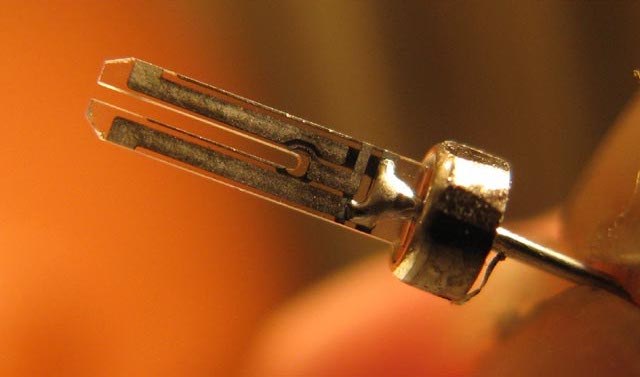
\includegraphics[width=\textwidth]{images/quartz-tuningfork.jpg}
        \end{column}
    \end{columns}
\end{frame}
\inlineslide{s:quartz-clocks}\label{l:quartz-clocks}
% Crystal image: https://pixabay.com/photos/rock-crystal-clear-to-white-gem-top-1603480/ (no attribution required)
% Tuning fork: https://commons.wikimedia.org/wiki/File:Inside_QuartzCrystal-Tuningfork.jpg (public domain)

Quartz clocks are cheap, but they are not totally accurate.
Due to manufacturing imperfections, some clocks run slightly faster than others.
Moreover, the oscillation frequency varies with the temperature.
Typical quartz clocks are tuned to be quite stable around room temperature, but significantly higher or lower temperatures slow down the clock.
The rate by which a clock runs fast or slow is called \emph{drift}.

\pagebreak[3]
\begin{frame}
    \label{s:quartz-drift}
    \frametitle{Quartz clock error: drift}
    \begin{itemize}
        \item One clock runs slightly fast, another slightly slow
        \item Drift measured in \textbf{parts per million} (ppm)
        \item 1~ppm = 1~microsecond/second = 86~ms/day = 32~s/year
        \item Most computer clocks correct within $\approx 50$~ppm\\[1em]
        % 50 ppm is about half an hour of drift per year
    \end{itemize}
    \begin{columns}
        \begin{column}{0.2\textwidth}
            Temperature significantly affects drift
        \end{column}
        \begin{column}{0.75\textwidth}
            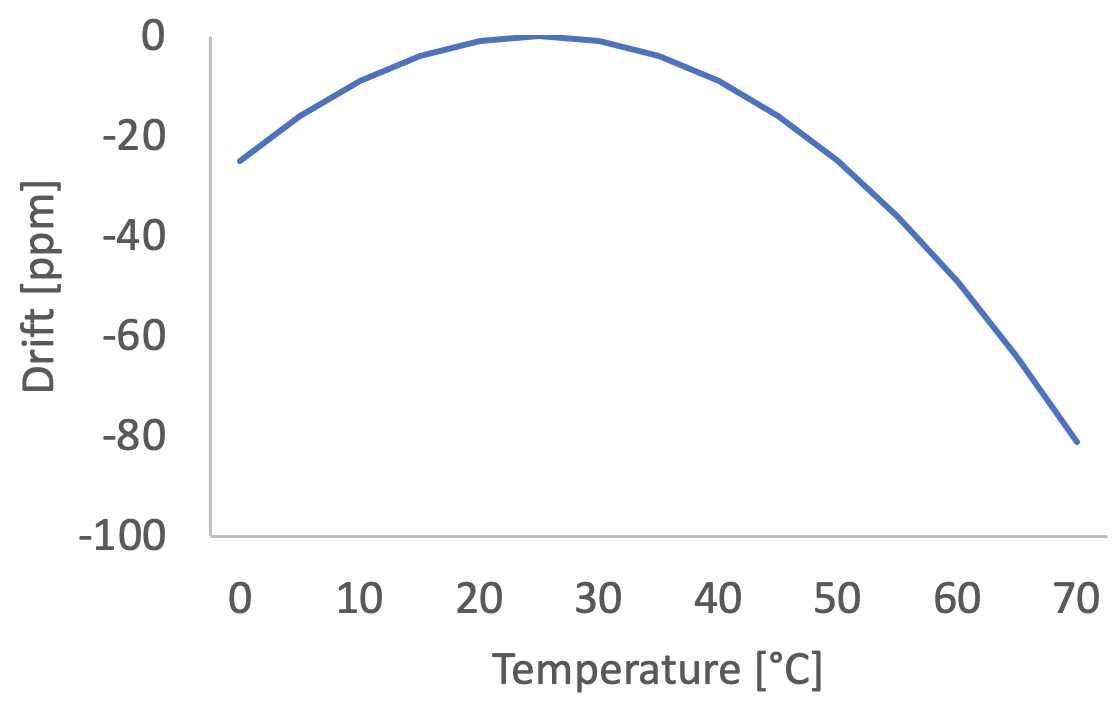
\includegraphics[width=\textwidth]{images/quartz-drift.png}
        \end{column}
    \end{columns}
\end{frame}
\inlineslide{s:quartz-drift}\label{l:quartz-drift}

\begin{frame}
    \label{s:atomic-clocks}
    \frametitle{Atomic clocks}
    \begin{columns}
        \begin{column}{0.5\textwidth}
            \begin{itemize}
                \item Caesium-133 has a resonance (``hyperfine transition'') at $\approx 9$~GHz
                \item Tune an electronic oscillator to that resonant frequency
                \item 1 second = 9,192,631,770 periods of that signal
                \item Accuracy $\approx 1 \text{ in } 10^{-14}$ (1 second in 3 million years)
                \item Price $\approx$ {\textsterling}20,000 (?)\\ (can get cheaper rubidium clocks for $\approx$ {\textsterling}1,000)
            \end{itemize}
        \end{column}
        \begin{column}{0.5\textwidth}
            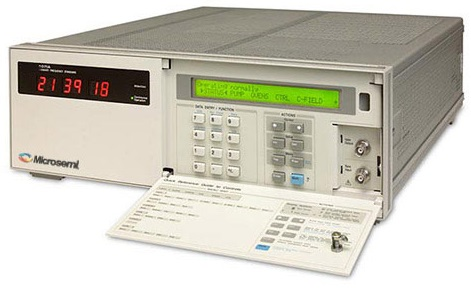
\includegraphics[width=\textwidth]{images/atomic-clock.jpg}\\[1em]
            \scriptsize\url{https://www.microsemi.com/product-directory/cesium-frequency-references/4115-5071a-cesium-primary-frequency-standard}
        \end{column}
    \end{columns}
\end{frame}
\inlineslide{s:atomic-clocks}\label{l:atomic-clocks}

When greater accuracy is required, atomic clocks are used.
These clocks are based on quantum-mechanical properties of certain atoms, such as caesium or rubidium.
In fact, the time unit of \emph{one second} in the International System of Units (SI) is defined to be exactly 9,192,631,770 periods of a particular resonant frequency of the caesium-133 atom.

\begin{frame}
    \label{s:gps-time}
    \frametitle{GPS as time source}
    \begin{columns}
        \begin{column}{0.5\textwidth}
            \begin{itemize}
                \item 31 satellites, each carrying an atomic clock
                \item satellite broadcasts current time and location
                \item calculate position from speed-of-light delay between satellite and receiver
                \item corrections for atmospheric effects, relativity, etc.
                \item in datacenters, need antenna on the roof
            \end{itemize}
        \end{column}
        \begin{column}{0.5\textwidth}
            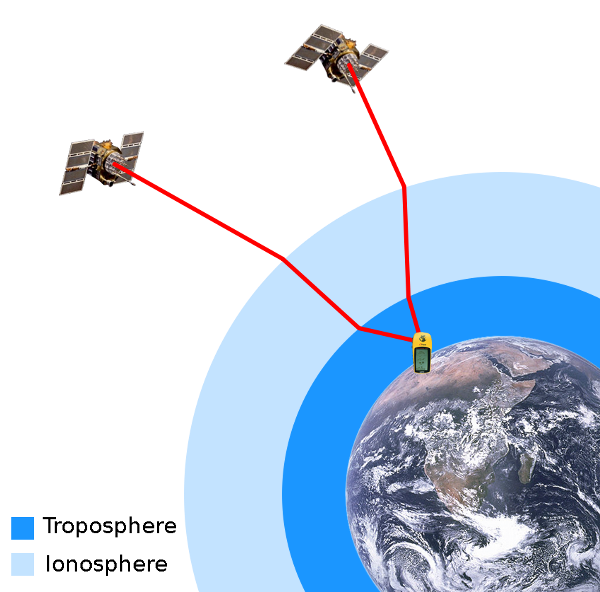
\includegraphics[width=\textwidth]{images/gps-satellites.png}\\[1em]
            \scriptsize\url{https://commons.wikimedia.org/wiki/File:Gps-atmospheric-efects.png}
        \end{column}
    \end{columns}
\end{frame}
\inlineslide{s:gps-time}\label{l:gps-time}

Another high-accuracy method of obtaining the time is to rely on the GPS satellite positioning system, or similar systems such as Galileo or GLONASS.
These systems work by having several satellites orbiting the Earth and broadcasting the current time at very high resolution.
Receivers measure the time it took the signal from each satellite to reach them, and use this to compute their distance from each satellite, and hence their location.
By connecting a GPS receiver to a computer, it is possible to obtain a clock that is accurate to within a fraction of a microsecond, provided that the receiver is able to get a clear signal from the satellites.
In a datacenter, there is generally too much electromagnetic interference to get a good signal, so a GPS receiver requires an antenna on the roof of the datacenter building.

We now have a problem: we have two different definitions of time~-- one based on quantum mechanics, the other based on astronomy~-- and those two definitions don't match up precisely.
One rotation of planet Earth around its own axis does not take exactly $24 \times 60 \times 60 \times \text{9,192,631,770}$ periods of caesium-133's resonant frequency.
In fact, the speed of rotation of the planet is not even constant: it fluctuates due to the effects of tides, earthquakes, glacier melting, and some unexplained factors.

\begin{frame}
    \label{s:utc}
    \frametitle{Coordinated Universal Time (UTC)}
    \begin{columns}
        \begin{column}{0.7\textwidth}
            \textbf{Greenwich Mean Time} (GMT, solar time): it's noon when the sun is in the south, as seen from the Greenwich meridian\\[1em]
            \uncover<2->{\textbf{International Atomic Time} (TAI): 1 day is
            $24 \times 60 \times 60 \times \text{9,192,631,770}$ periods of caesium-133's resonant frequency\\[1em]}
            \uncover<3->{\textbf{Problem}: speed of Earth's rotation is not constant\\[1em]}
            \uncover<4->{\textbf{Compromise}: UTC is TAI with corrections to account for Earth rotation\\[1em]}
            \uncover<5->{\textbf{Time zones} and \textbf{daylight savings time} are offsets to UTC}
        \end{column}
        \begin{column}{0.3\textwidth}
            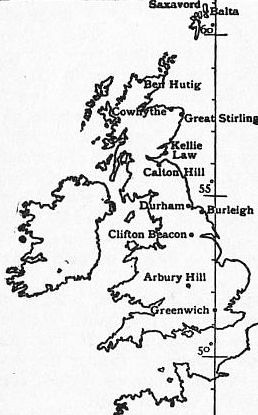
\includegraphics[width=\textwidth]{images/greenwich-meridian.jpg}
        \end{column}
    \end{columns}
\end{frame}
\inlineslide{s:utc}\label{l:utc}
% Image source: https://commons.wikimedia.org/wiki/File:Britannica_Figure_of_the_Earth.jpg (public domain)

The solution is \emph{Coordinated Universal Time} (UTC), which is based on atomic time, but includes corrections to account for variations in the Earth's rotation.
In everyday life we use our local \emph{time zone}, which is specified as an offset to UTC.

The UK's local time zone is called \emph{Greenwich Mean Time} (GMT) in winter, and \emph{British Summer Time} (BST) in summer, where GMT is defined to be equal to UTC, and BST is defined to be UTC~+~1~hour.
Confusingly, the term \emph{Greenwich Mean Time} was originally used to refer to mean solar time on the Greenwich meridian, i.e.\ it used to be defined in terms of astronomy, while now it is defined in terms of atomic clocks.
Today, the term \emph{UT1} is used to refer to mean solar time at 0{\textdegree} longitude.

The difference between UTC and TAI is that UTC includes \emph{leap seconds}, which are added as needed to keep UTC roughly in sync with the rotation of the Earth.

\begin{frame}
    \label{s:leap-seconds}
    \frametitle{Leap seconds}
    Every year, on 30 June and 31 December at 23:59:59 UTC, one of three things happens:
    \begin{itemize}
        \item The clock immediately jumps forward to 00:00:00, skipping one second (\textbf{negative leap second})
        \item The clock moves to 00:00:00 after one second, as usual
        \item The clock moves to 23:59:60 after one second, and then moves to 00:00:00 after one further second\\
            (\textbf{positive leap second})
    \end{itemize}
    This is announced several months beforehand.
    \begin{center}
        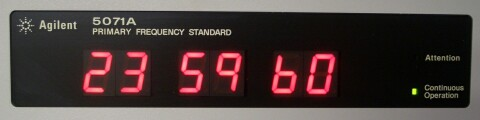
\includegraphics[width=8cm]{images/leap-second.jpg}
        \scriptsize\url{http://leapsecond.com/notes/leap-watch.htm}
    \end{center}
\end{frame}
\inlineslide{s:leap-seconds}\label{l:leap-seconds}

Due to leap seconds, it is not true that an hour always as 3600 seconds, and a day always has 86,400 seconds.
In the UTC timescale, a day can be 86,399 seconds, 86,400 seconds, or 86,401 seconds long due to a leap second.
This complicates software that needs to work with dates and times.

In computing, a \emph{timestamp} is a representation of a particular point in time.
Two representations of timestamps are commonly used: Unix time and ISO~8601.
For Unix time, zero corresponds to the arbitrarily chosen date of 1 January 1970, known as the \emph{epoch}.
There are minor variations: for example, Java's \verb|System.currentTimeMillis()| is like Unix time, but uses milliseconds rather than seconds.

\begin{frame}
    \label{s:time-representation}
    \frametitle{How computers represent timestamps}
    Two most common representations:
    \begin{itemize}
        \item \textbf{Unix time}: number of seconds since 1 January 1970 00:00:00 UTC (the ``epoch''), \emph{not counting leap seconds}
        \item \textbf{ISO 8601}: year, month, day, hour, minute, second, and timezone offset relative to UTC\\
            example: \texttt{\timestampexample}\\[1em]
    \end{itemize}\pause
    Conversion between the two requires:
    \begin{itemize}
        \item Gregorian calendar: 365 days in a year, except leap years\\
            \texttt{(year \% 4 == 0 \&\& (year \% 100 != 0 ||}\\
            \texttt{~~~~~~~~~~~~~~~~~~~year \% 400 == 0))}
        \item Knowledge of past and future leap seconds\dots?!
    \end{itemize}
\end{frame}
\inlineslide{s:time-representation}\label{l:time-representation}

To be correct, software that works with timestamps needs to know about leap seconds.
For example, if you want to calculate how many seconds elapsed between two timestamps, you need to know how many leap seconds were inserted between those two dates.
For dates that are more than about six months into the future, this is impossible to know, because the Earth's rotation has not happened yet!

The most common approach in software is to simply ignore leap seconds, pretend that they don't exist, and hope that the problem somehow goes away.
This approach is taken by Unix timestamps, and by the POSIX standard.
For software that only needs coarse-grained timings (e.g.\ rounded to the nearest day), this is fine, since the difference of a few seconds is not significant.

However, operating systems and distributed systems often \emph{do} rely on high-resolution timestamps for accurate measurements of time, where a difference of one second is very noticeable.
In such settings, ignoring leap seconds can be dangerous.
For example, say you have a Java program that twice calls \verb|System.currentTimeMillis()|, 500~ms apart, within a positive leap second (i.e.\ while the clock is saying 23:59:60).
What is the difference between those two timestamps going to be?
It can't be 500, since the \verb|currentTimeMillis()| clock does not account for leap seconds.
Does the clock stop, so the difference between the two timestamps is zero?
Or could the difference even be negative, so the clock runs backwards for a brief moment?
The documentation is silent about this question.
(The best solution is probably to use a \emph{monotonic clock} instead, which we introduce on \autoref{l:monotonic-clock}.)

Poor handling of the leap second on 30 June 2012 is what caused the simultaneous failures of many services on that day (\autoref{l:mystery}).
Due to a bug in the Linux kernel, the leap second had a high probability of triggering a livelock condition when running a multithreaded process \citep{Allen:2013,Minar:2012}.
Even a reboot did not fix the problem instead, but setting the system clock reset the bad state in the kernel.

\begin{frame}
    \label{s:leap-second-handling}
    \frametitle{How most software deals with leap seconds}
    \begin{columns}
        \begin{column}{0.7\textwidth}
            \textbf{By ignoring them!}\\[1em]
            \uncover<2->{However, OS and DistSys often need timings with sub-second accuracy.\\[1em]}
            \uncover<3->{30 June 2012: bug in Linux kernel caused livelock on leap second, causing many Internet services to go down\\[1em]}
            \uncover<4->{Pragmatic solution: ``\textbf{smear}'' (spread out) the leap second over the course of a day}
        \end{column}
        \begin{column}{0.3\textwidth}
            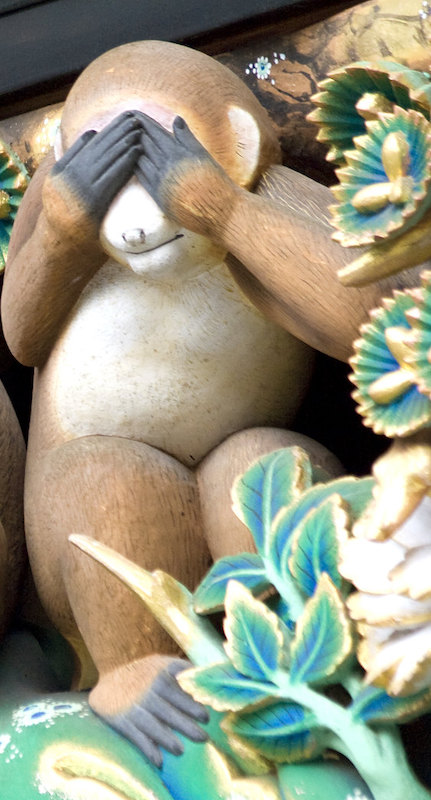
\includegraphics[width=\textwidth]{images/monkey.jpg}
            \scriptsize\url{https://www.flickr.com/photos/ru_boff/37915499055/}
        \end{column}
    \end{columns}
\end{frame}
\inlineslide{s:leap-second-handling}\label{l:leap-second-handling}

Today, some software handles leap seconds explicitly, while other programs continue to ignore them.
A pragmatic solution that is widely used today is that when a positive leap second occurs, rather than inserting it between 23:59:59 and 00:00:00, the extra second is spread out over several hours before and after that time by deliberately slowing down the clocks during that time (or speeding up in the case of a negative leap second).
This approach is called \emph{smearing} the leap second, and it is not without problems.
However, it is a pragmatic alternative to making all software aware of and robust to leap seconds, which may well be infeasible.

\supervision{
    Describe some problems that may arise from leap second smearing.
}{
    Measurements of time durations will be slightly wrong during the smearing period.
    For example, if the extra second is spread over 24 hours (12 hours before and 12 hours after the leap second), this amounts to an error of about 12~ppm in the rate at which clocks are running.
    However, many systems can tolerate this level of inaccuracy.

    A bigger problem is that if a timestamp from a smeared clock is compared with a non-smeared timestamp, there will be a spurious difference of up to half a second.
    For example, this could arise if two nodes with different smearing policies attempt to measure the network latency between them by sending one node's current timestamp as a message to the other node, and calculating the difference of timestamps when the message is received.
    The measured latency could even be negative.

    A similar problem arises (to a lesser degree) when comparing two timestamps from clocks that use different approaches to smearing.
    For example, some implementations of smearing spread the extra second over different periods of time.
    Also, different functions are used to interpolate across the leap second discontinuity: some systems use a linear functions, other use a cosine.
    There is no standardised approach to smearing.

    See \url{https://developers.google.com/time/smear} for some discussion.
    Our department's Markus Kuhn tried to get this standardised in 2006: \url{https://www.cl.cam.ac.uk/~mgk25/time/utc-sls/}
}

\subsection{Clock synchronisation and monotonic clocks}\label{sec:clock-sync}

\begin{frame}
    \label{s:clock-sync}
    \frametitle{Clock synchronisation}
    Computers track physical time/UTC with a quartz clock\\
    (with battery, continues running when power is off)\\[1em]
    Due to \textbf{clock drift}, clock error gradually increases\\[1em]\pause
    \textbf{Clock skew}: difference between two clocks at a point in time\\[1em]\pause
    \textbf{Solution}: Periodically get the current time from a server that has a more
    accurate time source (atomic clock or GPS receiver)\\[1em]
    Protocols: Network Time Protocol (\textbf{NTP}),\\ Precision Time Protocol (\textbf{PTP})
\end{frame}
\inlineslide{s:clock-sync}\label{l:clock-sync}

Atomic clocks are too expensive and bulky to build into every computer and phone, so quartz clocks are used.
As discussed on \autoref{l:quartz-drift}, these clocks drift, and need adjustment from time to time.
The most common approach is to use the \emph{Network Time Protocol} (NTP).
All mainstream operating systems have NTP clients built in; for example, \autoref{l:ntp-config} shows the NTP settings dialog in macOS.

\begin{frame}
    \label{s:ntp-config}
    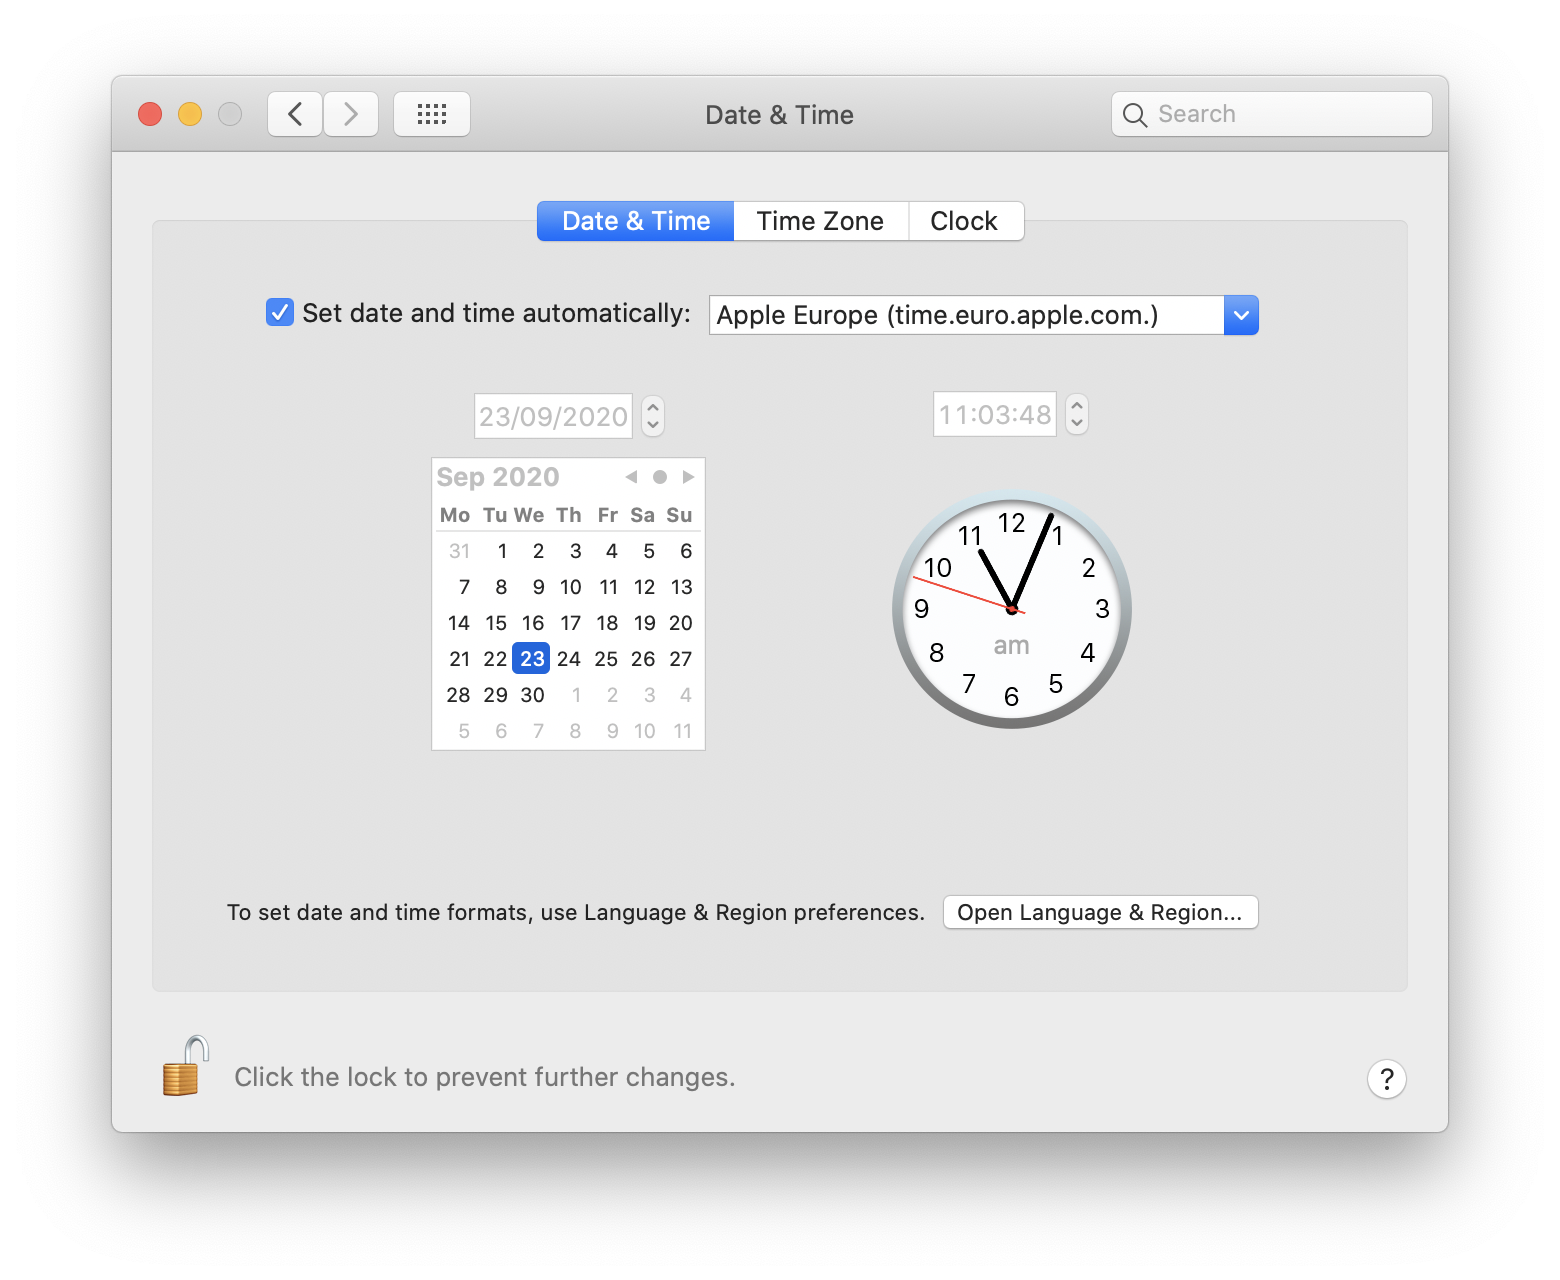
\includegraphics[height=\paperheight]{images/ntp-config.png}
\end{frame}
\inlineslide{s:ntp-config}\label{l:ntp-config}

\begin{frame}
    \label{s:ntp}
    \frametitle{Network Time Protocol (NTP)}
    Many operating system vendors run NTP servers,\\configure OS to use them by default\\[1em]\pause
    Hierarchy of clock servers arranged into \textbf{strata}:
    \begin{itemize}
        \item Stratum 0: atomic clock or GPS receiver
        \item Stratum 1: synced directly with stratum 0 device
        \item Stratum 2: servers that sync with stratum 1, etc.\\[1em]
    \end{itemize}\pause
    May contact multiple servers, discard outliers, average rest\\[1em]
    Makes multiple requests to the same server, use statistics to reduce random error due to variations in network latency\\[1em]
    Reduces clock skew to a few milliseconds in good network conditions, but can be much worse!
\end{frame}
\inlineslide{s:ntp}\label{l:ntp}

Time synchronisation over a network is made difficult by unpredictable latency.
As discussed on \autoref{l:timing-violations}, both network latency and nodes' processing speed can vary considerably.
To reduce the effects of random variations, NTP takes several samples of time measurements and applies statistical filters to eliminate outliers.

\autoref{l:ntp-calculation} shows how NTP estimates the clock skew between the client and the server.
When the client sends a request message, it includes the current timestamp $t_1$ according to the client's clock.
When the server receives the request, and before processing it, the server records the current timestamp $t_2$ according to the server's clock.
When the server sends its response, it echoes the value $t_1$ from the request, and also includes the server's receipt timestamp $t_2$ and the server's response timestamp $t_3$ in the reply.
Finally, when the client receives the response, it records the current timestamp $t_4$ according to the client's clock.

We can determine the time that the messages spent travelling across the network by calculating the round-trip time from the client's point of view ($t_4 - t_1$) and subtracting the processing time on the server ($t_3 - t_2$).
We then estimate the one-way network latency as being half of the total network delay.
Thus, by the time the response reaches the client, we can estimate that the server's clock will have moved on to $t_3$ plus the one-way network latency.
We then subtract the client's current time $t_4$ from the estimated server time to obtain the estimated skew between the two clocks.

This estimation depends on the assumption that the network latency is approximately the same in both directions.
This assumption is probably true if latency is dominated by geographic distance between client and server.
However, if queueing time in the network is a significant factor in the latency (e.g.\ if one node's network link is heavily loaded while the other node's link has plenty of spare capacity), then there could be a large difference between request and response latency.
Unfortunately, most networks do not give nodes any indication of the actual latency that a particular packet has experienced.

\begin{frame}
    \label{s:ntp-calculation}
    \frametitle{Estimating time over a network}
    \begin{center}
        \begin{tikzpicture}
            \node [rectangle,fill=red!10,draw] (client) at (0,3) {NTP client};
            \node [rectangle,fill=red!10,draw] (server) at (8,3) {NTP server};
            \draw (client) -- (0,0);
            \draw (server) -- (8,0);
            \draw<2-> [bigarrow] (0,2) --
                node [at start,left] {$t_1$}
                node [above,sloped] {request: $t_1$}
                node [at end,right] {$t_2$} (8,1.5);
            \draw<3-> [bigarrow] (8,1) --
                node [at start,right] {$t_3$}
                node [above,sloped] {response: $(t_1, t_2, t_3)$}
                node [at end,left] {$t_4$} (0,0.5);
        \end{tikzpicture}
    \end{center}
    \uncover<4->{ \[ \text{Round-trip network delay: } \delta = (t_4 - t_1) - (t_3 - t_2)\] }
    \uncover<5->{ \[ \text{Estimated server time when client receives response: } t_3 + \frac{\delta}{2} \] }
    \uncover<6->{ \[ \text{Estimated clock skew: }\theta = t_3 + \frac{\delta}{2} - t_4 = \frac{t_2 - t_1 + t_3 - t_4}{2} \] }
\end{frame}
\inlineslide{s:ntp-calculation}\label{l:ntp-calculation}

\supervision{
    What is the maximum possible error in the NTP client's estimate of skew with regard to one particular server, assuming that both nodes correctly follow the protocol?
}{
    The maximum possible error in $\theta$ is $\delta/2$.
    This occurs either in the extreme case where request latency is 0 and response latency is $\delta$, or in the other extreme case where request latency is $\delta$ and response latency is 0.
    Whenever latency is nonzero, the error will be less than $\delta/2$.
}

Once NTP has estimated the clock skew between client and server, the next step is to adjust the client's clock to bring it in line with the server.
The method used for this depends on the amount of skew.
The client corrects small differences gently by adjusting the clock speed to run slightly faster or slower as needed, which gradually reduces the skew over the course of a few minutes.
This process is called \emph{slewing} the clock.

\autoref{l:ntp-graph} shows an example of slewing, in which the client's clock frequency converges to the same rate as the server, keeping the two in sync to within a few milliseconds.
Of course, the exact accuracy achieved in a particular system depends on the timing properties of the network between client and server.

However, if the skew is larger, slewing would take too long, so the NTP client instead forcibly sets its clock to the estimated correct time based on the server timestamp.
This is called \emph{stepping} the clock.
Any applications that are watching the clock on the client will see time suddenly jump forwards or backwards.

And finally, if the skew is very large (by default, more than about 15 minutes), the NTP client may decide that something must be wrong, and refuse to adjust the clock, leaving the problem for a user or operator to correct.
For this reason, any system that depends on clock synchronisation needs to be carefully monitored for clock skew: just because a node is running NTP, that does not guarantee that its clock will be correct, since it could get stuck in a panic state in which it refuses to adjust the clock.

\begin{frame}
    \label{s:ntp-slew}
    \frametitle{Correcting clock skew}
    Once the client has estimated the clock skew $\theta$, it needs to apply that correction to its clock.\\
    \begin{itemize}
        \item If $|\theta| < 125$~ms, \textbf{slew} the clock:\\
            slightly speed it up or slow it down by up to 500~ppm\\
            (brings clocks in sync within $\approx$ 5 minutes)\\[1em]\pause
        \item If $125\text{ ms} \le |\theta| < \text{1,000 s}$, \textbf{step} the clock:\\
            suddenly reset client clock to estimated server timestamp\\[1em]\pause
        \item If $|\theta| \ge \text{1,000 s}$, \textbf{panic} and do nothing\\
            (leave the problem for a human operator to resolve)\\[1em]
    \end{itemize}
    Systems that rely on clock sync need to monitor clock skew!
\end{frame}
\inlineslide{s:ntp-slew}\label{l:ntp-slew}

\begin{frame}
    \label{s:ntp-graph}
    \begin{center}
        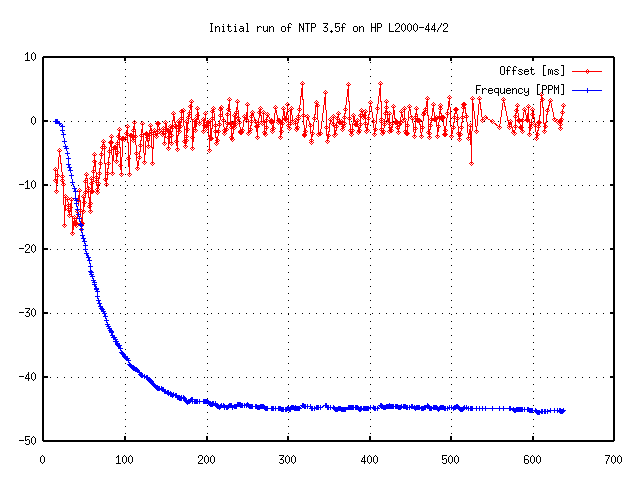
\includegraphics[height=8cm]{images/ntp-graph.png}
        \scriptsize\url{http://www.ntp.org/ntpfaq/NTP-s-algo.htm}
    \end{center}
\end{frame}
\inlineslide{s:ntp-graph}\label{l:ntp-graph}

The fact that clocks may be stepped by NTP, i.e.\ suddenly moved forwards or backwards, has an important implication for any software that needs to measure elapsed time.
\autoref{l:monotonic-clock} shows an example in Java, in which we want to measure the running time of a function \verb|doSomething()|.
Java has two core functions for getting the current timestamp from the operating system's local clock: \verb|currentTimeMillis()| and \verb|nanoTime()|.
Besides the different resolution (milliseconds versus nanoseconds), the key difference between the two is how they behave in the face of clock adjustments from NTP or other sources.

\verb|currentTimeMillis()| is a \emph{time-of-day} clock (also known as \emph{real-time} clock) that returns the time elapsed since a fixed reference point (in this case, the Unix epoch of 1 January 1970).
When the NTP client steps the local clock, a time-of-day clock may jump.
Thus, if you use such a clock to measure elapsed time, the resulting difference between end timestamp and start timestamp may be much greater than the actual elapsed time (if the clock was stepped forwards), or it may even be negative (if the clock was stepped backwards).
This type of clock is therefore not suitable for measuring elapsed time.

On the other hand, \verb|nanoTime()| is a \emph{monotonic} clock, which is not affected by NTP stepping: it still counts seconds elapsed, but it always moves forward.
Only the rate at which it moves forward may be adjusted by NTP slewing.
This makes a monotonic clock much more robust for measuring elapsed time.
The downside is that a timestamp from a monotonic clock is meaningless by itself: it measures the time since some arbitrary reference point, such as the time since this computer was started up.
When using a monotonic clock, only the difference between two timestamps from the same node is meaningful.
It does not make sense to compare monotonic clock timestamps across different nodes.

\begin{frame}
    \label{s:monotonic-clock}
    \frametitle{Monotonic and time-of-day clocks}
    \inputminted{java}{code/nonmonotonic.java}
    \begin{tikzpicture}[remember picture,overlay]
        \node (dosomething) [xshift=-2.2cm,yshift=1.8cm] at (current page.center) {};
        \node<2-> (stepping) [xshift=2.5cm,yshift=-0.5cm,red] at (current page.center) {NTP client steps the clock during this};
        \draw<2-> [-Stealth,red,line width=4pt] (stepping) .. controls +(0,2) and +(2,0) .. (dosomething);
    \end{tikzpicture}
    \uncover<3->{\inputminted{java}{code/monotonic.java}}
\end{frame}
\inlineslide{s:monotonic-clock}\label{l:monotonic-clock}

Most operating systems and programming languages provide both a time-of-day clock and a monotonic clock, since both are useful for different purposes.

\begin{frame}
    \label{s:monotonic-comparison}
    \frametitle{Monotonic and time-of-day clocks}
    \textbf{Time-of-day clock:}
    \begin{itemize}
        \item<1-> Time since a fixed date (e.g.\ 1 January 1970 epoch)
        \item<2-> May suddenly move forwards or backwards (NTP stepping), subject to leap second adjustments
        \item<3-> Timestamps can be compared across nodes (if synced)
        \item<4-> Java: \texttt{System.currentTimeMillis()}
        \item<4-> Linux: \texttt{clock\char`_gettime(CLOCK\char`_REALTIME)}\\[1em]
    \end{itemize}
    \textbf{Monotonic clock:}
    \begin{itemize}
        \item<1-> Time since arbitrary point (e.g.\ when machine booted up)
        \item<2-> Always moves forwards at near-constant rate
        \item<3-> Good for measuring elapsed time on a single node
        \item<4-> Java: \texttt{System.nanoTime()}
        \item<4-> Linux: \texttt{clock\char`_gettime(CLOCK\char`_MONOTONIC)}
    \end{itemize}
\end{frame}
\inlineslide{s:monotonic-comparison}\label{l:monotonic-comparison}

\subsection{Causality and happens-before}\label{sec:causality}

We will now move on to the problem of ordering events in a distributed system, which is closely related to the concept of time.
Consider the scenario on \autoref{l:moon-cheese}, in which user A makes a statement $m_1$ and sends it as a message to the other two users, B and C.
On receiving $m_1$, user B reacts by sending a reply $m_2$ to the other two users, A and C.
However, even if we assume the network links are reliable, they allow reordering (\autoref{l:model-network}), so C might receive $m_2$ before $m_1$ if $m_1$ is slightly delayed in the network.

From C's point of view, the result is confusing: C first sees the reply, and then the message it is replying to.
It almost looks as though B was able to see into the future and anticipate A's statement before A even said it.
In real life this sort of reordering of spoken words does not happen, and so we intuitively don't expect it to happen in computer systems either.

As a more technical example, consider $m_1$ to be an instruction that creates an object in a database, and $m_2$ to be an instruction that updates this same object.
If a node processes $m_2$ before $m_1$ it would first attempt to update a nonexistent object, and then create an object which would not subsequently be updated.
The database instructions only make sense if $m_1$ is processed before $m_2$.

\begin{frame}
    \label{s:moon-cheese}
    \frametitle{Ordering of messages}
    \begin{center}
        \begin{tikzpicture}
            \node [rectangle,fill=red!10,draw] (user1) at (0,3.7) {user A};
            \node [rectangle,fill=red!10,draw] (user2) at (4,3.7) {user B};
            \node [rectangle,fill=red!10,draw] (user3) at (8,3.7) {user C};
            \draw (user1) -- (0,0.2);
            \draw (user2) -- (4,0.2);
            \draw (user3) -- (8,0.2);
            \draw<1-> [bigarrow] (0,3.0)
                .. node [above,sloped] {$m_1$} controls (2,2.75) .. (4,2.5)
                .. controls (5,2.375) and (5,0.875) .. (6,0.75) -- (8,0.5);
            \draw<1-> [bigarrow] (0,2.9)
                .. controls (1,2.775) and (1,2.3) .. (2,2.05)
                -- node [above,sloped] {$m_1$} (4,1.8);
            \draw<2-> [bigarrow] (4,1.5) -- node [above,sloped] {$m_2$} (8,1.0);
            \draw<2-> [bigarrow] (4,1.4) -- node [above,sloped] {$m_2$} (0,0.9);
        \end{tikzpicture}
    \end{center}
    \uncover<1->{$m_1 = $ ``A says: The moon is made of cheese!''}\\
    \uncover<2->{$m_2 = $ ``B says: Oh no it isn't!''}\\[1em]%
    \uncover<3->{C sees $m_2$ first, $m_1$ second,\\even though logically $m_1$ \textbf{happened before} $m_2$.}
\end{frame}
\inlineslide{s:moon-cheese}\label{l:moon-cheese}

How can C determine the correct order in which it should put the messages?
A monotonic clock won't work since its timestamps are not comparable across nodes.
A first attempt might be to get a timestamp from a time-of-day clock whenever a user wants to send a message, and to attach that timestamp to the message.
In this scenario, we might reasonably expect $m_2$ to have a later timestamp than $m_1$, since $m_2$ is a response to $m_1$ and so $m_2$ must have happened after $m_1$.

Unfortunately, in a partially synchronous system model, this does not work reliably.
The clock synchronisation performed by NTP and similar protocols always leaves some residual uncertainty about the exact skew between two clocks, especially if the network latency in the two directions is asymmetric.
We therefore cannot rule out the following scenario: A sends $m_1$ with timestamp $t_1$ according to A's clock.
When B receives $m_1$, the timestamp according to B's clock is $t_2$, where $t_2 < t_1$, because A's clock is slightly ahead of B's clock.
Thus, if we order messages based on their timestamps from time-of-day clocks, we might again end up with the wrong order.

\begin{frame}<1-2>[label=physical-order]
    \label{s:physical-order}
    \frametitle<1-2>{Ordering of messages using timestamps?}
    \frametitle<3>{Physical timestamps inconsistent with causality}
    \begin{center}
        \begin{tikzpicture}
            \node [rectangle,fill=red!10,draw] (user1) at (0,3.7) {user A};
            \node [rectangle,fill=red!10,draw] (user2) at (4,3.7) {user B};
            \node [rectangle,fill=red!10,draw] (user3) at (8,3.7) {user C};
            \draw (user1) -- (0,0.2);
            \draw (user2) -- (4,0.2);
            \draw (user3) -- (8,0.2);
            \draw [bigarrow] (0,3.0)
                .. node [above,sloped] {$m_1$} node [at start,left,fill=yellow!50] {$t_1$} controls (2,2.75) .. (4,2.5)
                .. controls (5,2.375) and (5,0.875) .. (6,0.75) -- (8,0.5);
            \draw [bigarrow] (0,2.9)
                .. controls (1,2.775) and (1,2.3) .. (2,2.05)
                -- node [above,sloped] {$m_1$} node [at end,right,fill=yellow!50] {$t_2$} (4,1.8);
            \draw [bigarrow] (4,1.5) -- node [above,sloped] {$m_2$} (8,1.0);
            \draw [bigarrow] (4,1.4) -- node [above,sloped] {$m_2$} (0,0.9);
        \end{tikzpicture}
    \end{center}
    $m_1 = (t_1, \text{``A says: The moon is made of cheese!''})$\\
    $m_2 = (t_2, \text{``B says: Oh no it isn't!''})$\\[1em]%
    \uncover<2->{\textbf{Problem}: even with synced clocks, $t_2 < t_1$ is possible.\\
    Timestamp order is inconsistent with expected order!}
\end{frame}
\inlineslide{s:physical-order}\label{l:physical-order}

To formalise what we mean with the ``correct'' order in this type of scenario, we use the \emph{happens-before relation} as defined on \autoref{l:happens-before}.
This definition assumes that each node has only a single thread of execution, so for any two execution steps of a node, it is clear which one happened first.
More formally, we assume that there is a \emph{strict total order} on the events that occur at the same node.
A multithreaded process can be modelled by using a separate node to represent each thread.

We then extend this order across nodes by defining that a message is sent before that same message is received (in other words, we rule out time travel: it is not possible to receive a message that has not yet been sent).
For convenience, we assume that every sent message is unique, so when a message is received, we always know unambiguously where and when that message was sent.
In practice, duplicate messages may exist, but we can make them unique, for example by including the ID of the sender node and a sequence number in each message.

Finally, we take the transitive closure, and the result is the happens-before relation.
This is a \emph{partial order}, which means that it is possible that for some events $a$ and $b$, neither $a$ happened before $b$, nor $b$ happened before $a$.
In that case, we call $a$ and $b$ \emph{concurrent}.
Note that here, ``concurrent'' does not mean literally ``at the same time'', but rather that $a$ and $b$ are independent in the sense that there is no sequence of messages leading from one to the other.

\begin{frame}
    \label{s:happens-before}
    \frametitle{The happens-before relation}
    An \textbf{event} is something happening at one node (sending or receiving a message, or a local execution step).\\[1em]
    We say event $a$ \textbf{happens before} event $b$ (written $a \rightarrow b$) iff:\pause
    \begin{itemize}
        \item $a$ and $b$ occurred at the same node, and $a$ occurred before $b$ in that node's local execution order; or\pause
        \item event $a$ is the sending of some message $m$, and event $b$ is the receipt of that same message $m$ (assuming sent messages are unique); or\pause
        \item there exists an event $c$ such that $a \rightarrow c$ and $c \rightarrow b$.\\[1em]\pause
    \end{itemize}
    The happens-before relation is a partial order:
    it is possible that neither $a \rightarrow b$ nor $b \rightarrow a$.
    In that case, $a$ and $b$ are \textbf{concurrent} (written $a \parallel b$).
\end{frame}
\inlineslide{s:happens-before}\label{l:happens-before}

\begin{frame}
    \label{s:hb-example}
    \frametitle{Happens-before relation example}
    \begin{center}
        \begin{tikzpicture}
            \node [rectangle,fill=red!10,draw] (A) at (0,3.7) {A};
            \node [rectangle,fill=red!10,draw] (B) at (4,3.7) {B};
            \node [rectangle,fill=red!10,draw] (C) at (8,3.7) {C};
            \draw (A) -- (0,0.5);
            \draw (B) -- (4,0.5);
            \draw (C) -- (8,0.5);
            \tikzstyle{event}=[circle,fill=black,inner sep=2pt]
            \node (a) [event] at (0,3.0) {}; \draw (a) node [left,xshift=-0.1cm] {$a$};
            \node (b) [event] at (0,2.5) {}; \draw (b) node [left,xshift=-0.1cm] {$b$};
            \node (c) [event] at (4,2.0) {}; \draw (c) node [right,xshift=0.1cm] {$c$};
            \node (d) [event] at (4,1.5) {}; \draw (d) node [left,xshift=-0.1cm] {$d$};
            \node (e) [event] at (8,2.8) {}; \draw (e) node [right,xshift=0.1cm] {$e$};
            \node (f) [event] at (8,1.0) {}; \draw (f) node [right,xshift=0.1cm] {$f$};
            \draw [bigarrow] (b) -- node[above] {$m_1$} (c);
            \draw [bigarrow] (d) -- node[above] {$m_2$} (f);
        \end{tikzpicture}
    \end{center}\pause
    \begin{itemize}
        \item $a \rightarrow b$, $c \rightarrow d$, and $e \rightarrow f$ due to node execution order\pause
        \item $b \rightarrow c$ and $d \rightarrow f$ due to messages $m_1$ and $m_2$\pause
        \item $a \rightarrow c$, $a \rightarrow d$, $a \rightarrow f$, $b \rightarrow d$, $b \rightarrow f$,
            and $c \rightarrow f$ due to transitivity\pause
        \item $a \parallel e$, $b \parallel e$, $c \parallel e$, and $d \parallel e$
    \end{itemize}
\end{frame}
\inlineslide{s:hb-example}\label{l:hb-example}

\supervision{\label{q:strict-partial-order}
    A relation $R$ is a \emph{strict partial order} if it is irreflexive ($\nexists a.\; (a,a) \in R$) and transitive ($\forall a,b,c.\; (a,b) \in R \wedge (b,c) \in R \Longrightarrow (a,c) \in R$).
    Prove that the happens-before relation is a strict partial order.
    You may assume that any two nodes are a nonzero distance apart, as well as the physical principle that information cannot travel faster than the speed of light.
}{
    The fact that happens-before is transitive follows directly from the third bullet point of its definition.

    To prove that it is irreflexive, we use proof by contradiction.
    Assume to the contrary that there exists $a$ such that $a \rightarrow a$.
    This implies at least one of the following:
    \begin{enumerate}
        \item $a$ occurred before $a$ in some node's local execution order.
            However, this contradicts our assumption that every node's local execution forms a strict total order, which is irreflexive.
        \item $a$ is the sending of some message $m$, and $a$ is the receipt of that same message $m$.
            This is impossible because sending and receiving a message are two different events.
        \item There exists an event $b$ such that $a \rightarrow b$ and $b \rightarrow a$.
            Let $N_a$ be the node at which $a$ occurs, and $N_b$ the node at which $b$ occurs.
            Then either $N_a = N_b$ or $N_a \neq N_b$.
            If $N_a = N_b$ then $a \rightarrow b$ and $b \rightarrow a$ contradict our assumption that every node's local execution forms a strict total order, so we have $N_a \neq N_b$.

            Let $t_a$ be the time at which $a$ occurs and let $t_b$ be the time at which $b$ occurs, both according to $N_a$'s clock.
            Let $d$ be the distance in space between $N_a$ and $N_b$.
            $a \rightarrow b$ implies the existence of a message, or a sequence of messages (possibly via other nodes), through which information can travel from $a$ to $b$.
            Since this information cannot travel faster than the speed of light, we have $t_b \ge t_a + \frac{d}{c}$, where $c$ is the speed of light.
            By similar argument, $b \rightarrow a$ implies that $t_a \ge t_b + \frac{d}{c}$.

            Since we are assuming $d > 0$ and the speed of light is finite, $\frac{d}{c} > 0$.
            Therefore we have $t_b > t_a$ and $t_a > t_b$, a contradiction.
    \end{enumerate}
}

\supervision{\label{q:hb-three-cases}
    Show that for any two events $a$ and $b$, exactly one of the three following statements must be true: either $a \rightarrow b$, or $b \rightarrow a$, or $a \parallel b$.
}{
    The statement $a \rightarrow b$ must be either true or false.
    If it is true, then it is not the case that $a \parallel b$ by definition.
    Moreover, since the happens-before relation is a strict partial order (\autoref{q:strict-partial-order}), $a \rightarrow b$ implies $b \not\rightarrow a$.

    If $a \not\rightarrow b$, consider the statement $b \rightarrow a$, which must be either true or false.
    If it is true, then it is not the case that $a \parallel b$ by definition.
    If it is false, then $a \parallel b$ by definition.

    In all cases examined, exactly one of the three statements $\{a \rightarrow b,\; b \rightarrow a,\; a \parallel b\}$ is true.
}

The happens-before relation is a way of reasoning about \emph{causality} in distributed systems.
Causality considers whether information could have flowed from one event to another, and thus whether one event may have influenced another.
In the example of \autoref{l:moon-cheese}, $m_2$ (``Oh no it isn't!'') is a reply to $m_1$ (``The moon is made of cheese!''), and so $m_1$ influenced $m_2$.
Whether one event truly ``caused'' another is a philosophical question that we don't need to answer now; what matters for our purposes is that the sender of $m_2$ had already received $m_1$ at the time of sending $m_2$.

\begin{frame}
    \label{s:causality}
    \frametitle{Causality}
    Taken from physics (relativity).
    \begin{itemize}
        \item When $a \rightarrow b$, then $a$ \textbf{might have caused} $b$.
        \item When $a \parallel b$, we know that $a$ \textbf{cannot have caused} $b$.
    \end{itemize}
    Happens-before relation encodes \textbf{potential causality}.\pause
    \begin{center}
        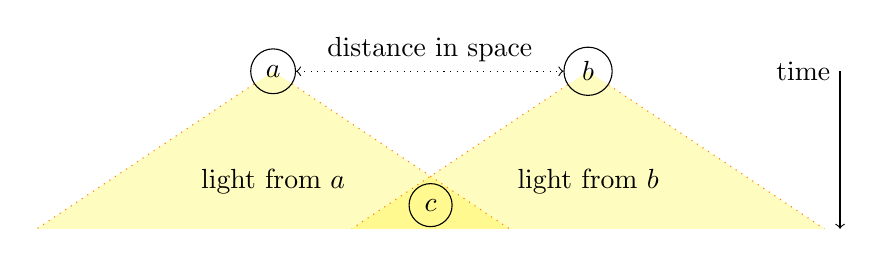
\begin{tikzpicture}
            \fill<3-> [yellow,nearly transparent] (0,2) -- (3,0) -- (-3,0) -- cycle;
            \fill<4-> [yellow,nearly transparent] (4,2) -- (7,0) -- (1,0) -- cycle;
            \node<2-> (a) [circle,draw] at (0,2) {$a$};
            \node<2-> (b) [circle,draw] at (4,2) {$b$};
            \node<5-> (c) [circle,draw] at (2,0.3) {$c$};
            \draw<2-> [<->,dotted] (a) -- node [above] {distance in space} (b);
            \draw<3-> [orange,dotted] (a) -- (-3,0);
            \draw<3-> [orange,dotted] (a) -- (3,0);
            \draw<4-> [orange,dotted] (b) -- (1,0);
            \draw<4-> [orange,dotted] (b) -- (7,0);
            \node<3-> at (0,0.6) {light from $a$};
            \node<4-> at (4,0.6) {light from $b$};
            \draw<2-> [->] (7.2,2) -- node [at start,left] {time} (7.2,0);
            \node at (-3,0) {}; \node at (7.2,2.2) {}; % placeholder so that slide 1 doesn't jump
        \end{tikzpicture}
    \end{center}
    \uncover<6->{Let $\prec$ be a strict total order on events.\\
    If $(a \rightarrow b) \Longrightarrow (a \prec b)$ then $\prec$ is a \textbf{causal order}\\
    (or: $\prec$ is ``consistent with causality'').\\
    NB. ``causal'' $\neq$ ``casual''!}
\end{frame}
\inlineslide{s:causality}\label{l:causality}

The notion of causality is borrowed from physics, where it is generally believed that it is not possible for information to travel faster than the speed of light.
Thus, if you have two events $a$ and $b$ that occur sufficiently far apart in space, but close together in time, then it is impossible for a signal sent from $a$ to arrive at $b$'s location before event $b$, and vice versa.
Therefore, $a$ and $b$ must be \emph{causally unrelated}.

An event $c$ that is sufficiently close in space to $a$, and sufficiently long after $a$ in time, will be within $a$'s \emph{light cone}: that is, it is possible for a signal from $a$ to reach $c$, and therefore $a$ might influence $c$.
In distributed systems, we usually work with messages on a network rather than beams of light, but the principle is very similar.

% "causality is reachability in spacetime"
% https://twitter.com/palvaro/status/1233208997257170944


\section{Broadcast protocols and logical time}\label{sec:broadcast}

\begin{frame}
    \begin{center}
        Lecture 4\\[2em]
        \Large{\color{darkblue}{Broadcast protocols and logical time}}
    \end{center}
\end{frame}

In this lecture we will examine \emph{broadcast protocols} (also known as \emph{multicast protocols}), that is, algorithms for delivering one message to multiple recipients.
These are a useful building blocks for higher-level distributed algorithms, as we will see in \autoref{sec:replication}.

Several different broadcast protocols are used in practice, and their main difference is the \emph{order} in which they deliver messages.
As we saw in the last lecture, the concept of ordering is closely related to clocks and time.
Hence we will start this lecture by examining more closely how clocks can help us keep track of ordering within a distributed system.

\subsection{Logical time}\label{sec:logical-time}

\againframe<3>{physical-order}

Physical clocks, which we discussed in \autoref{sec:physical-clocks}, measure the number of seconds elapsed.
However, recall that on \autoref{l:physical-order}, we saw that timestamps from physical clocks can be inconsistent with causality, even if those clocks are synchronised using something like NTP.
That is, if $\mathsf{send}(m)$ is the event of sending message $m$, and if the happens-before relation indicates that $\mathsf{send}(m_1) \rightarrow \mathsf{send}(m_2)$, then it could nevertheless be the case that the the physical timestamp of $\mathsf{send}(m_1)$ (according to the clock of $m_1$'s sender) is less than the physical timestamp of $\mathsf{send}(m_2)$ (according to the clock of $m_2$'s sender).

In contrast, \emph{logical clocks} focus on correctly capturing the order of events in a distributed system.

\begin{frame}
    \label{s:logical-clocks}
    \frametitle{Logical vs. physical clocks}
    \begin{itemize}
        \item Physical clock: count number of \textbf{seconds elapsed}
        \item Logical clock: count number of \textbf{events occurred}\\[1em]
    \end{itemize}
    Physical timestamps: useful for many things, but may be \textbf{inconsistent with causality}.\\[1em]\pause
    Logical clocks: designed to \textbf{capture causal dependencies}.
    \[ (e_1 \rightarrow e_2) \Longrightarrow (T(e_1) < T(e_2)) \]\pause
    We will look at two types of logical clocks:
    \begin{itemize}
        \item Lamport clocks
        \item Vector clocks
    \end{itemize}
\end{frame}
\inlineslide{s:logical-clocks}\label{l:logical-clocks}

The first type of logical clock we will examine is the Lamport clock, introduced by \citet{Lamport:1978} in one of the seminal papers of distributed computing.

\begin{frame}
    \label{s:lamport-definition}
    \frametitle{Lamport clocks algorithm}
    \begin{algorithmic}
        \On{initialisation}
            \State $t := 0$ \Comment{each node has its own local variable $t$}
        \EndOn
        \State
        \On{any event occurring at the local node}
            \State $t := t + 1$
        \EndOn
        \State
        \On{request to send message $m$}
            \State $t := t + 1$; send $(t, m)$ via the underlying network link
        \EndOn
        \State
        \On{receiving $(t', m)$ via the underlying network link}
            \State $t := \mathrm{max}(t, t') + 1$
            \State deliver $m$ to the application
        \EndOn
    \end{algorithmic}
\end{frame}
\inlineslide{s:lamport-definition}\label{l:lamport-definition}

\begin{frame}
    \label{s:lamport-description}
    \frametitle{Lamport clocks in words}
    \begin{itemize}
        \item Each node maintains a counter $t$,\\incremented on every local event $e$
        \item Let $L(e)$ be the value of $t$ after that increment
        \item Attach current $t$ to messages sent over network
        \item Recipient moves its clock forward to timestamp in the message (if greater than local counter), then increments\\[1em]
    \end{itemize}\pause
    Properties of this scheme:
    \begin{itemize}
        \item If $a \rightarrow b$ then $L(a) < L(b)$\pause
        \item However, $L(a) < L(b)$ does not imply $a \rightarrow b$\pause
        \item Possible that $L(a) = L(b)$ for $a \neq b$
    \end{itemize}
\end{frame}
\inlineslide{s:lamport-description}\label{l:lamport-description}

A Lamport timestamp is essentially an integer that counts the number of events that have occurred.
As such, it has no direct relationship to physical time.
On each node, time increases because the integer is incremented on every event.
The algorithm assumes a crash-stop model (or a crash-recovery model if the timestamp is maintained in stable storage, i.e.\ on disk).

When a message is sent over the network, the sender attaches its current Lamport timestamp to that message.
In the example on \autoref{l:lamport-example}, $t=2$ is attached to $m_1$ and $t=4$ is attached to $m_2$.
When the recipient receives a message, it moves its local Lamport clock forward to the timestamp in the message plus one; if the recipient's clock is already ahead of the timestamp in the message, it is only incremented.

Lamport timestamps have the property that if $a$ happened before $b$, then $b$ always has a greater timestamp than $a$; in other words, the timestamps are consistent with causality.
However, the converse is not true: in general, if $b$ has a greater timestamp than $a$, we know that $b \not\rightarrow a$, but we do not know whether it is the case that $a \rightarrow b$ or that $a \parallel b$.

It is also possible for two different events to have the same timestamp.
In the example on \autoref{l:lamport-example}, the third event on node $A$ and the first event on node $B$ both have a timestamp of 3.
If we need a unique timestamp for every event, each timestamp can be extended with the name or identifier of the node on which that event occurred.
Within the scope of a single node, each event is assigned a unique timestamp; thus, assuming each node has a unique name, the combination of timestamp and node name is globally unique (across all nodes).

\begin{frame}
    \label{s:lamport-example}
    \frametitle{Lamport clocks example}
    \begin{center}
        \begin{tikzpicture}
            \node [rectangle,fill=red!10,draw] (A) at (0,3.7) {A};
            \node [rectangle,fill=red!10,draw] (B) at (4,3.7) {B};
            \node [rectangle,fill=red!10,draw] (C) at (8,3.7) {C};
            \draw (A) -- (0,0.5);
            \draw (B) -- (4,0.5);
            \draw (C) -- (8,0.5);
            \tikzstyle{event}=[circle,fill=black,inner sep=2pt]
            \node (a) [event] at (0,3.0) {};
            \node (b) [event] at (0,2.5) {};
            \node (c) [event] at (4,2.0) {};
            \node (d) [event] at (4,1.5) {};
            \node (e) [event] at (8,2.8) {};
            \node (f) [event] at (8,1.0) {};
            \node (g) [event] at (0,1.5) {};
            \draw<1-2| handout:0> (a) node [left,xshift=-0.1cm] {1};
            \draw<1-2| handout:0> (b) node [left,xshift=-0.1cm] {2};
            \draw<1-2| handout:0> (c) node [right,xshift=0.1cm] {3};
            \draw<1-2| handout:0> (d) node [left,xshift=-0.1cm] {4};
            \draw<1-2| handout:0> (e) node [right,xshift=0.1cm] {1};
            \draw<1-2| handout:0> (f) node [right,xshift=0.1cm] {5};
            \draw<1-2| handout:0> (g) node [left,xshift=-0.1cm] {3};
            \draw<3-> (a) node [left,xshift=-0.1cm] {$(1, A)$};
            \draw<3-> (b) node [left,xshift=-0.1cm] {$(2, A)$};
            \draw<3-> (c) node [right,xshift=0.1cm] {$(3, B)$};
            \draw<3-> (d) node [left,xshift=-0.1cm] {$(4, B)$};
            \draw<3-> (e) node [right,xshift=0.1cm] {$(1, C)$};
            \draw<3-> (f) node [right,xshift=0.1cm] {$(5, C)$};
            \draw<3-> (g) node [left,xshift=-0.1cm] {$(3, A)$};
            \draw [bigarrow] (b) -- node[above] {$(2, m_1)$} (c);
            \draw [bigarrow] (d) -- node[below] {$(4, m_2)$} (f);
        \end{tikzpicture}
    \end{center}
    \uncover<2->{Let $N(e)$ be the node at which event $e$ occurred.\\
    Then the pair $(L(e), N(e))$ \textbf{uniquely identifies} event $e$.}\\[1em]%
    \uncover<4->{Define a \textbf{total order} $\prec$ using Lamport timestamps:
    \[ (a \prec b) \Longleftrightarrow (L(a) < L(b) \;\vee\; (L(a) = L(b) \;\wedge\; N(a) < N(b))) \]
    This order is \textbf{causal}: $(a \rightarrow b) \Longrightarrow (a \prec b)$}
\end{frame}
\inlineslide{s:lamport-example}\label{l:lamport-example}

Recall that the happens-before relation is a partial order (\autoref{l:happens-before}).
Using Lamport timestamps we can extend this partial order into a \emph{total order}.
We use the lexicographic order over (timestamp, node name) pairs: that is, we first compare the timestamps, and if they are the same, we break ties by comparing the node names.

This relation $\prec$ puts all events into a linear order: for any two events $a \neq b$ we have either $a \prec b$ or $b \prec a$.
It is a causal order: that is, whenever $a \rightarrow b$ we have $a \prec b$.
In other words, $\prec$ is a \emph{linear extension} of the partial order $\rightarrow$.
However, if $a \parallel b$ we could have either $a \prec b$ or $b \prec a$, so the order of the two events is determined arbitrarily by the algorithm.

\supervision{\label{q:lamport-example}
    Given the sequence of messages in the following execution, show the Lamport timestamps at each send or receive event.

    \begin{center}
    \begin{tikzpicture}
        \node [rectangle,fill=red!10,draw] (A) at (0,7) {A};
        \node [rectangle,fill=red!10,draw] (B) at (3,7) {B};
        \node [rectangle,fill=red!10,draw] (C) at (6,7) {C};
        \node [rectangle,fill=red!10,draw] (D) at (9,7) {D};
        \draw (A) -- (0,0.7);
        \draw (B) -- (3,0.7);
        \draw (C) -- (6,0.7);
        \draw (D) -- (9,0.7);
        \tikzstyle{event}=[circle,fill=black,inner sep=2pt]
        \node (s1) [event] at (0,6.5) {};
        \node (r1) [event] at (3,6.2) {};
        \node (s2) [event] at (0,6.0) {};
        \node (r2) [event] at (6,5.4) {};
        \node (s3) [event] at (0,5.5) {};
        \node (r3) [event] at (9,4.6) {};
        \node (s4) [event] at (3,4.7) {};
        \node (r4) [event] at (9,4.1) {};
        \node (s5) [event] at (3,4.2) {};
        \node (r5) [event] at (6,3.9) {};
        \node (s6) [event] at (6,3.4) {};
        \node (r6) [event] at (9,3.1) {};
        \node (s7) [event] at (6,2.9) {};
        \node (r7) [event] at (0,2.3) {};
        \node (s8) [event] at (0,1.8) {};
        \node (r8) [event] at (3,1.5) {};
        \node (s9) [event] at (6,1.3) {};
        \node (r9) [event] at (3,1.0) {};
        \draw [bigarrow] (s1) -- node[above] {$m_1$} (r1);
        \draw [bigarrow] (s2) -- node[above,pos=0.25] {$m_2$} (r2);
        \draw [bigarrow] (s3) -- node[above,pos=0.17] {$m_3$} (r3);
        \draw [bigarrow] (s4) -- node[above,pos=0.25] {$m_4$} (r4);
        \draw [bigarrow] (s5) -- node[above] {$m_5$} (r5);
        \draw [bigarrow] (s6) -- node[above] {$m_6$} (r6);
        \draw [bigarrow] (s7) -- node[above,pos=0.25] {$m_7$} (r7);
        \draw [bigarrow] (s8) -- node[above] {$m_8$} (r8);
        \draw [bigarrow] (s9) -- node[above] {$m_9$} (r9);
    \end{tikzpicture}
    \end{center}
}{
    The following table shows both the Lamport timestamps from this exercise and the vector timestamps from \autoref{q:vector-example}.

    % Based on Steven Hand & Robert Watson's problem sheet
    \begin{center}
    \begin{tabular}{|c|cccc|cccc|}
    \hline
    Message & \multicolumn{4}{c|}{Lamport} & \multicolumn{4}{c|}{Vector} \\
            &  A &  B &  C &  D            & A & B & C & D \\
    \hline
    initial &  0 & 0  &  0 &  0            & $\langle 0, 0, 0, 0 \rangle$
                                           & $\langle 0, 0, 0, 0 \rangle$
                                           & $\langle 0, 0, 0, 0 \rangle$
                                           & $\langle 0, 0, 0, 0 \rangle$ \\
    \hline
    $m_1$   &  1 &  2 & -- & --            & $\langle 1, 0, 0, 0 \rangle$
                                           & $\langle 1, 1, 0, 0 \rangle$
                                           & --
                                           & -- \\
    $m_2$   &  2 & -- &  3 & --            & $\langle 2, 0, 0, 0 \rangle$
                                           & --
                                           & $\langle 2, 0, 1, 0 \rangle$
                                           & -- \\
    $m_3$   &  3 & -- & -- &  4            & $\langle 3, 0, 0, 0 \rangle$
                                           & --
                                           & --
                                           & $\langle 3, 0, 0, 1 \rangle$ \\
    $m_4$   & -- &  3 & -- &  5            & --
                                           & $\langle 1, 2, 0, 0 \rangle$
                                           & --
                                           & $\langle 3, 2, 0, 2 \rangle$ \\
    $m_5$   & -- &  4 &  5 & --            & --
                                           & $\langle 1, 3, 0, 0 \rangle$
                                           & $\langle 2, 3, 2, 0 \rangle$
                                           & -- \\
    $m_6$   & -- & -- &  6 &  7            & --
                                           & --
                                           & $\langle 2, 3, 3, 0 \rangle$
                                           & $\langle 3, 3, 3, 3 \rangle$ \\
    $m_7$   &  8 & -- &  7 & --            & $\langle 4, 3, 4, 0 \rangle$
                                           & --
                                           & $\langle 2, 3, 4, 0 \rangle$
                                           & -- \\
    $m_8$   &  9 & 10 & -- & --            & $\langle 5, 3, 4, 0 \rangle$
                                           & $\langle 5, 4, 4, 0 \rangle$
                                           & --
                                           & -- \\
    $m_9$   & -- & 11 &  8 & --            & --
                                           & $\langle 5, 5, 5, 0 \rangle$
                                           & $\langle 2, 3, 5, 0 \rangle$
                                           & -- \\
    \hline
    final   &  9 & 11 &  8 & 7             & $\langle 5, 3, 4, 0 \rangle$
                                           & $\langle 5, 5, 5, 0 \rangle$
                                           & $\langle 2, 3, 5, 0 \rangle$
                                           & $\langle 3, 3, 3, 3 \rangle$ \\
    \hline
    \end{tabular}
    \end{center}
}

\supervision{
    Prove that the total order $\prec$ using Lamport timestamps is a causal order.
}{
    We assume $a \rightarrow b$ for some events $a$ and $b$.
    Because the happens-before relation is a strict partial order (\autoref{q:strict-partial-order}) we have $a \neq b$.
    To show that $a \prec b$ we use induction over the recursive structure of the definition of the happens-before relation.
    That is, we consider three cases:
    \begin{enumerate}
        \item First base case: $a \rightarrow b$ because $a$ and $b$ occurred at the same node, and $a$ occurred before $b$ in that node's local execution order.
            Then $L(a) < L(b)$ because the algorithm for Lamport timestamps only ever increases a node's local clock, and every local event increases the clock, so an event that occurs later in a node's local execution must have a greater timestamp.
            Hence $a \prec b$.
        \item Second base case: $a \rightarrow b$ because $a = \mathsf{send}(m)$ and $b = \mathsf{receive}(m)$ for some message $m$.
            Then $L(a)$ is included in the message $m$, and so $L(b) = \mathrm{max}(t, L(a)) + 1 > L(a)$ by the definition of the Lamport timestamp algorithm.
            Therefore $L(a) < L(b)$ and hence $a \prec b$.
        \item Inductive step: $a \rightarrow b$ because there exists an event $c$ such that $a \rightarrow c$ and $c \rightarrow b$.
            Then $a \prec c$ and $c \prec b$ by the inductive hypothesis.
            Since $\prec$ is a total order, it is transitive, and therefore $a \prec b$.
    \end{enumerate}
}

Given the Lamport timestamps of two events, it is in general not possible to tell whether those events are concurrent or whether one happened before the other.
If we do want to detect when events are concurrent, we need a different type of logical time: a \emph{vector clock}.

While Lamport timestamps are just a single integer (possibly with a node name attached), vector timestamps are a list of integers, one for each node in the system.
By convention, if we put the $n$ nodes into a vector $\langle N_1, N_2, \dots, N_n \rangle$, then a vector timestamp is a similar vector $\langle t_1, t_2, \dots, t_n \rangle$ where $t_i$ is the entry corresponding to node $N_i$.
Concretely, $t_i$ is the number of events known to have occurred at node $N_i$.

In a vector $T = \langle t_1, t_2, \dots, t_n \rangle$ we refer to element $t_i$ as $T[i]$, like an index into an array.

\begin{frame}
    \label{s:vector-clocks}
    \frametitle{Vector clocks}
    Given Lamport timestamps $L(a)$ and $L(b)$ with $L(a) < L(b)$\\we can't tell whether $a \rightarrow b$ or $a \parallel b$.\\[1em]
    If we want to detect which events are concurrent, we need \textbf{vector clocks}:\pause
    \begin{itemize}
        \item Assume $n$ nodes in the system, $N = \langle N_1, N_2, \dots, N_n \rangle$\pause
        \item Vector timestamp of event $a$ is $V(a) = \langle t_1, t_2, \dots, t_n\rangle$
        \item $v_i$ is number of events observed by node $N_i$\pause
        \item Each node has a current vector timestamp $T$
        \item On event at node $N_i$, increment vector element $T[i]$\pause
        \item Attach current vector timestamp to each message
        \item Recipient merges message vector into its local vector
    \end{itemize}
\end{frame}
\inlineslide{s:vector-clocks}\label{l:vector-clocks}

Apart from the difference between a scalar and a vector, the vector clock algorithm is very similar to a Lamport clock (compare \autoref{l:lamport-definition} and \autoref{l:vector-definition}).
A node initialises its vector clock to contain a zero for each node in the system.
Whenever an event occurs at node $N_i$, it increments the $i$th entry (its own entry) in its vector clock.
When a message is sent over the network, the sender's current vector timestamp is attached to the message.
Finally, when a message is received, the recipient merges the vector timestamp in the message with its local timestamp by taking the element-wise maximum of the two vectors, and then the recipient increments its own entry.

\begin{frame}
    \label{s:vector-definition}
    \frametitle{Vector clocks algorithm}
    \begin{algorithmic}
        \On{initialisation at node $N_i$}
            \State $T := \langle 0, 0, \dots, 0 \rangle$ \Comment{local variable at node $N_i$}
        \EndOn
        \State
        \On{any event occurring at node $N_i$}
            \State $T[i] := T[i] + 1$
        \EndOn
        \State
        \On{request to send message $m$ at node $N_i$}
            \State $T[i] := T[i] + 1$; send $(T, m)$ via network
        \EndOn
        \State
        \On{receiving $(T', m)$ at node $N_i$ via the network}
            \State $T[j] := \mathrm{max}(T[j], T'[j])$ for every $j \in \{1, \dots, n\}$
            \State $T[i] := T[i] + 1$; deliver $m$ to the application
        \EndOn
    \end{algorithmic}
\end{frame}
\inlineslide{s:vector-definition}\label{l:vector-definition}

\autoref{l:vector-example} shows an example of this algorithm in action.
Note that when $C$ receives message $m_2$ from $B$, the vector entry for $A$ is also updated to 2 because this event has an indirect causal dependency on the two events that happened at $A$.
In this way, the vector timestamps mirror the transitivity of the happens-before relation.

\begin{frame}
    \label{s:vector-example}
    \frametitle{Vector clocks example}
    Assuming the vector of nodes is $N = \langle A, B, C \rangle$:
    \begin{center}
        \begin{tikzpicture}
            \node [rectangle,fill=red!10,draw] (A) at (0,3.7) {A};
            \node [rectangle,fill=red!10,draw] (B) at (4,3.7) {B};
            \node [rectangle,fill=red!10,draw] (C) at (8,3.7) {C};
            \draw (A) -- (0,0.5);
            \draw (B) -- (4,0.5);
            \draw (C) -- (8,0.5);
            \tikzstyle{event}=[circle,fill=black,inner sep=2pt]
            \node (a) [event] at (0,3.0) {};
            \node (b) [event] at (0,2.5) {};
            \node (c) [event] at (4,2.0) {};
            \node (d) [event] at (4,1.5) {};
            \node (e) [event] at (8,2.8) {};
            \node (f) [event] at (8,1.0) {};
            \node (g) [event] at (0,1.5) {};
            \draw (a) node [left,xshift=-0.1cm] {$\langle 1, 0, 0 \rangle$};
            \draw (b) node [left,xshift=-0.1cm] {$\langle 2, 0, 0 \rangle$};
            \draw (c) node [right,xshift=0.1cm] {$\langle 2, 1, 0 \rangle$};
            \draw (d) node [left,xshift=-0.1cm] {$\langle 2, 2, 0 \rangle$};
            \draw (e) node [right,xshift=0.1cm] {$\langle 0, 0, 1 \rangle$};
            \draw (f) node [right,xshift=0.1cm] {$\langle 2, 2, 2 \rangle$};
            \draw (g) node [left,xshift=-0.1cm] {$\langle 3, 0, 0 \rangle$};
            \draw [bigarrow] (b) -- node[above,sloped] {$(\langle 2, 0, 0 \rangle, m_1)$} (c);
            \draw [bigarrow] (d) -- node[below,sloped] {$(\langle 2, 2, 0 \rangle, m_2)$} (f);
        \end{tikzpicture}
    \end{center}\pause
    The vector timestamp of an event $e$ represents a set of events, $e$ and its causal dependencies:
    $ \{e\} \cup \{a \mid a \rightarrow e\} $\\[1em]
    For example, $\langle 2, 2, 0\rangle$ represents the first two events from A, the first two events from B, and no events from C.
\end{frame}
\inlineslide{s:vector-example}\label{l:vector-example}

\begin{frame}
    \label{s:vector-ordering}
    \frametitle{Vector clocks ordering}
    Define the following order on vector timestamps\\(in a system with $n$ nodes):
    \begin{itemize}
        \item $T = T'$ iff $T[i] = T'[i]$ for all $i \in \{1, \dots, n\}$
        \item $T \le T'$ iff $T[i] \le T'[i]$ for all $i \in \{1, \dots, n\}$
        \item $T < T'$ iff $T \le T'$ and $T \ne T'$
        \item $T \parallel T'$ iff $T \not\le T'$ and $T' \not\le T$\\[1em]
    \end{itemize}\pause
    $V(a) \le V(b)$ iff $(\{a\} \cup \{e \mid e \rightarrow a\}) \subseteq (\{b\} \cup \{e \mid e \rightarrow b\})$\\[1em]\pause
    Properties of this order:
    \begin{itemize}
        \item $(V(a) < V(b)) \Longleftrightarrow (a \rightarrow b)$
        \item $(V(a) = V(b)) \Longleftrightarrow (a = b)$
        \item $(V(a) \parallel V(b)) \Longleftrightarrow (a \parallel b)$
    \end{itemize}
\end{frame}
\inlineslide{s:vector-ordering}\label{l:vector-ordering}

We then define a partial order over vector timestamps as shown on \autoref{l:vector-ordering}.
We say that one vector is less than or equal to another vector if every element of the first vector is less than or equal to the corresponding element of the second vector.
One vector is strictly less than another vector if they are less than or equal, and if they differ in at least one element.
However, two vectors are incomparable if one vector has a greater value in one element, and the other has a greater value in a different element.
For example, $T = \langle 2, 2, 0\rangle$ and $T' = \langle 0, 0, 1\rangle$ are incomparable because $T[1] > T'[1]$ but $T[3] < T'[3]$.

The partial order over vector timestamps corresponds exactly to the partial order defined by the happens-before relation.
Thus, the vector clock algorithm provides us with a mechanism for computing the happens-before relation in practice.

\supervision{\label{q:vector-example}
    Given the same sequence of messages as in \autoref{q:lamport-example}, show the vector clocks at each send or receive event.
}{
    See solution notes for \autoref{q:lamport-example}.
}

\supervision{\label{q:vector-happens-before}
    Using the Lamport and vector timestamps calculated in \autoref{q:lamport-example} and \ref{q:vector-example}, state whether or not the following events can be determined to have a happens-before relationship.

    \begin{center}
    \begin{tabular}{|c|c|c|c|}
    \hline
    \multicolumn{2}{|c|}{Events}                & Lamport & Vector \\
    \hline
    $\mathsf{send}(m_2)$ & $\mathsf{send}(m_3)$ &         &        \\
    $\mathsf{send}(m_3)$ & $\mathsf{send}(m_5)$ &         &        \\
    $\mathsf{send}(m_5)$ & $\mathsf{send}(m_9)$ &         &        \\
    \hline
    \end{tabular}
    \end{center}
}{
    Note that although Lamport clocks cannot determine \emph{happens-before} between nodes, they actually are sufficient to do so within a single node, as a higher local logical time will always reflect a later event.

    \begin{center}
    \begin{tabular}{|c|c|c|c|}
    \hline
    \multicolumn{2}{|c|}{Events}                & Lamport     & Vector \\
    \hline
    $\mathsf{send}(m_2)$ & $\mathsf{send}(m_3)$ & $2 < 3$     & $\langle 2, 0, 0, 0 \rangle <         \langle 3, 0, 0, 0 \rangle$ \\
    $\mathsf{send}(m_3)$ & $\mathsf{send}(m_5)$ & cannot tell & $\langle 3, 0, 0, 0 \rangle \parallel \langle 1, 3, 0, 0 \rangle$ \\
    $\mathsf{send}(m_5)$ & $\mathsf{send}(m_9)$ & cannot tell & $\langle 1, 3, 0, 0 \rangle <         \langle 2, 3, 5, 0 \rangle$ \\
    \hline
    \end{tabular}
    \end{center}
}

% TODO include this exercise? it's a bit hard though.
%\supervision{
%    Prove that the partial order over vector clocks is equivalent to the happens-before relation when vector clocks are computed according to the algorithm above.
%}{
%    We show that $(V(a) < V(b)) \Longleftrightarrow (a \rightarrow b)$ by proving the implication in both directions.
%
%    First, assume that $V(a) < V(b)$, i.e.\ $\forall i.\; V(a)[i] \le V(b)[i]$ and $\exists i.\; V(a)[i] < V(b)[i]$.
%    To prove that $a \rightarrow b$, note that in the vector clock algorithm, the only time when a node updates a vector entry other than its own %is on receiving a vector timestamp over the network.
%}

% Adapted from Robert Watson and Steven Hand's exercise sheet
\supervision{
    We have seen several types of physical clocks (time-of-day clocks with NTP, monotonic clocks) and logical clocks.
    For each of the following uses of time, explain which type of clock is the most appropriate: process scheduling; I/O; distributed filesystem consistency; cryptographic certificate validity; concurrent database updates.
}{
    \begin{description}
        \item [Process scheduling:]
            If we are talking about the operating system scheduler on a single machine, we only need to measure elapsed time (e.g.\ how many milliseconds a particular thread has been running), so a monotonic clock is the most appropriate.
            However, if we are talking about tasks scheduled to run on a particular date at a particular time (e.g.\ using the Unix service \texttt{cron}), a synchronised time-of-day clock is required.
        \item [I/O:]
            Timeouts and retry timers only need to measure elapsed time, so a monotonic clock is fine.
        \item [Distributed filesystem consistency:]
            When tracking file changes, we need to ensure that changes are consistent with causality, which requires a logical clock.
            Probably a vector clock is most appropriate, because it would allow detecting when two different users concurrently modify the same file.

            However, some software also relies on physical last-modification timestamps in a filesystem: for example, \texttt{make(1)} determines whether a file needs to be recompiled based on whether the source file's last-modification-time is earlier or later than that of the compilation output file.
            If the source file is written on one node but the compilation is performed on another node, this requires modification timestamps to be consistent with causality.
            It is also possible that a source file edit happens concurrently with a compilation, which could only be detected using vector clocks.
            However, last-modification timestamps are conventionally taken from a time-of-day clock, and changing these to be vector clocks would introduce compatibility problems.
        \item [Cryptographic certificate validity:]
            A certificate includes a start date (when it becomes valid) and end date (when it ceases to be valid).
            If a node wants to check whether it is within that period, a synchronised time-of-day clock is required.
        \item [Concurrent database updates:]
            Say two clients concurrently read the same object, modify it, and then write back the modified object to the database.
            The database will want to distinguish this from the situation where first client $A$ reads and writes the object, and then client $B$ reads and writes the object (where the version read by $B$ includes $A$'s changes).
            In the first case, the two updates are concurrent, while in the second case, B's update happened after A's update, so B's update should overwrite A's update.
            Distinguishing these two cases requires vector clocks.

            An alterative approach is that the database does not detect whether updates are concurrent, but simply always lets an update with a greater timestamp overwrite an update with a lesser timestamp.
            In this case, Lamport clocks are best, since they provide a total order that is consistent with causality.
    \end{description}
}

This completes our discussion of logical time.
We have seen two key algorithms: Lamport clocks and vector clocks, one providing a total order and the other capturing the partial order of happens-before.
Various other constructions have been proposed: for example, there are hybrid clocks that combine some of the properties of logical and physical clocks \citep{Kulkarni:2014}.

\subsection{Delivery order in broadcast protocols}\label{sec:delivery-order}

Many networks provide point-to-point (unicast) messaging, in which a message has one specified recipient.
We will now look at \emph{broadcast protocols}, which generalise networking such that a message is sent to \emph{all} nodes in some group.
The group membership may be fixed, or the system may provide mechanisms for nodes to join and leave the group.

Some local-area networks provide multicast or broadcast at the hardware level (for example, \emph{IP multicast}), but communication over the Internet typically only allows unicast.
Moreover, hardware-level multicast is typically provided on a \emph{best-effort} basis, which allows messages to be dropped; making it reliable requires retransmission protocols similar to those discussed here.

The system model assumptions about node behaviour (\autoref{l:model-nodes}) and synchrony (\autoref{l:model-synchrony}) carry over directly to broadcast groups.

\begin{frame}
    \label{s:broadcast-intro}
    \frametitle{Broadcast protocols}
    Broadcast (multicast) is \textbf{group communication}:
    \begin{itemize}
        \item One node sends message, all nodes in group deliver it\pause
        \item Set of group members may be fixed (static) or dynamic\pause
        \item If one node is faulty, remaining group members carry on\pause
        \item Note: concept is more general than IP multicast\\
            (we build upon point-to-point messaging)\\[1em]\pause
    \end{itemize}
    Build upon system models from lecture 2:
    \begin{itemize}
        \item Can be \textbf{best-effort} (may drop messages) or \\
            \textbf{reliable} (non-faulty nodes deliver every message,\\
            by retransmitting dropped messages)\pause
        \item Asynchronous/partially synchronous timing model\\
            $\Longrightarrow$ \textbf{no upper bound} on message latency
    \end{itemize}
\end{frame}
\inlineslide{s:broadcast-intro}\label{l:broadcast-intro}

Before we go into the details, we should clarify some terminology.
When an application wants to send a message to all nodes in the group, it uses an algorithm to \emph{broadcast} it.
To make this happen, the broadcast algorithm then \emph{sends} some messages to other nodes over point-to-point links, and another node \emph{receives} such a message when it arrives over the point-to-point link.
Finally, the broadcast algorithm may \emph{deliver} the message to the application.
As we shall see shortly, there is sometimes a delay between the time when a message is received and when it is delivered.

\begin{frame}
    \label{s:receive-deliver}
    \frametitle{Receiving versus delivering}
    \begin{tikzpicture}[every node/.style={font=\footnotesize,align=center}]
        \node at (0,4.4) {Node $A$:};
        \node at (6,4.4) {Node $B$:};
        \node [rectangle,draw,text width=4cm] (app1) at (0,3.6) {Application};
        \node [rectangle,draw,text width=4cm] (app2) at (6,3.6) {Application};
        \node [rectangle,draw,text width=4cm] (mid1) at (0,1.8) {Broadcast algorithm\\(middleware)};
        \node [rectangle,draw,text width=4cm] (mid2) at (6,1.8) {Broadcast algorithm\\(middleware)};
        \node [rectangle,draw,text width=10cm] (net) at (3,0) {Network};
        \draw<2-> [bigarrow] (app1)     -- node [left,orange]  {\textbf{broadcast}} (mid1);
        \draw<3-> [bigarrow] (-0.5,1.3) -- node [left,red]     {\textbf{send}}      (-0.5,0.25);
        \draw<3-> [bigarrow] (0.5,0.25) -- node [right,violet] {\textbf{receive}}   (0.5,1.3);
        \draw<3-> [bigarrow] (5.5,1.3)  -- node [left,red]     {\textbf{send}}      (5.5,0.25);
        \draw<3-> [bigarrow] (6.5,0.25) -- node [right,violet] {\textbf{receive}}   (6.5,1.3);
        \draw<4-> [bigarrow] (mid2)     -- node [right,blue]   {\textbf{deliver}}   (app2);
    \end{tikzpicture}\\[1em]%
    \uncover<3->{Assume network provides point-to-point \textbf{\color{red}send}/\textbf{\color{violet}receive}}\\[1em]%
    \uncover<4->{After broadcast algorithm \textbf{\color{violet}receives} message from network,
    it may buffer/queue it before \textbf{\color{blue}delivering} to the application}
\end{frame}
\inlineslide{s:receive-deliver}\label{l:receive-deliver}

We will examine three different forms of broadcast.
All of these are \emph{reliable}: every message is eventually delivered to every non-faulty node, with no timing guarantees.
However, they differ in terms of the order in which messages may be delivered at each node.
It turns out that this difference in ordering has very fundamental consequences for the algorithms that implement the broadcast.

\begin{frame}
    \label{s:broadcast-order}
    \frametitle{Forms of reliable broadcast}
    \textbf{FIFO broadcast}:\\
    If $m_1$ and $m_2$ are broadcast by the same node, and $\mathsf{broadcast}(m_1) \rightarrow \mathsf{broadcast}(m_2)$, then $m_1$ must be delivered before $m_2$\\[1em]\pause
    \textbf{Causal broadcast}:\\
    If $\mathsf{broadcast}(m_1) \rightarrow \mathsf{broadcast}(m_2)$ then $m_1$ must be delivered before $m_2$\\[1em]\pause
    \textbf{Total order broadcast}:\\
    If $m_1$ is delivered before $m_2$ on one node, then $m_1$ must be delivered before $m_2$ on all nodes\\[1em]\pause
    \textbf{FIFO-total order broadcast}:\\
    Combination of FIFO broadcast and total order broadcast
\end{frame}
\inlineslide{s:broadcast-order}\label{l:broadcast-order}

The weakest type of broadcast is called \emph{FIFO broadcast}, which is closely related to FIFO links (see \autoref{q:fifo-links}).
In this model, messages sent by the same node are delivered in the order they were sent.
For example, on \autoref{l:fifo-broadcast}, $m_1$ must be delivered before $m_3$, since they were both sent by $A$.
However, $m_2$ can be delivered at any time before, between, or after $m_1$ and $m_3$.

Another detail about these broadcast protocols: we assume that whenever a node broadcasts a message, it also delivers that message to itself (represented as a loopback arrow on \autoref{l:fifo-broadcast}).
This may seem unnecessary at first~-- after all, a node knows what messages it has itself broadcast!~-- but we will need this for total order broadcast.

\begin{frame}
    \label{s:fifo-broadcast}
    \frametitle{FIFO broadcast}
    \begin{center}
        \begin{tikzpicture}
            \node [rectangle,fill=red!10,draw] (A) at (0,4.7) {A};
            \node [rectangle,fill=red!10,draw] (B) at (4,4.7) {B};
            \node [rectangle,fill=red!10,draw] (C) at (8,4.7) {C};
            \draw (A) -- (0,0);
            \draw (B) -- (4,0);
            \draw (C) -- (8,0);
            % broadcast m1
            \node [inner sep=2pt] (send1) at (0,4) {};
            \path<1-> [->,very thick] (send1) edge [leftloop] node {$m_1$} (send1);
            \draw<1-4| handout: 0> [bigarrow] (0,4.0) -- node [above,near start] {$m_1$} (8,3.2);
            \draw<5-> [bigarrow,darkgreen] (0,4.0)
                .. node [above] {$m_1$} controls (2,3.8) .. (6,3.4)
                .. controls (7,3.3) and (7,1.4) .. (8,1.3);
            \draw<1-> [bigarrow] (0,3.9)
                .. controls (1,3.8) and (1,3.2) .. (2,3.1)
                -- node [above] {$m_1$} (4,2.9);
            % broadcast m2
            \node [inner sep=3pt] (send2) at (4,2.2) {};
            \path<2-> [->,very thick] (send2) edge [rightloop] node [yshift=0.2cm] {$m_2$} (send2);
            \draw<2-> [bigarrow] (4,2.4) -- node [above] {$m_2$} (0,2.0);
            \draw<2-> [bigarrow] (4,2.3) -- node [above] {$m_2$} (8,1.9);
            % broadcast m3
            \node [inner sep=2pt] (send3) at (0,1.5) {};
            \path<3-> [->,very thick] (send3) edge [leftloop] node {$m_3$} (send3);
            \draw<3-> [bigarrow] (0,1.5) -- node [above,near start] {$m_3$} (8,0.7);
            \draw<3-> [bigarrow] (0,1.4)
                .. controls (1,1.3) and (1,0.7) .. (2,0.6)
                -- node [above] {$m_3$} (4,0.4);
        \end{tikzpicture}
    \end{center}%
    \uncover<4->{Messages sent by the same node must be delivered in the order they were sent.\\
    Messages sent by different nodes can be delivered in any order.}\\%
    \uncover<5->{Valid orders: $(m_2, m_1, m_3)$ or $(m_1, m_2, m_3)$ or $(m_1, m_3, m_2)$}
\end{frame}
\inlineslide{s:fifo-broadcast}\label{l:fifo-broadcast}

The example execution on \autoref{l:fifo-broadcast} is valid FIFO broadcast, but it violates causality: node $C$ delivers $m_2$ before $m_1$, even though $B$ broadcast $m_2$ after delivering $m_1$.
\emph{Causal broadcast} provides a stricter ordering property than FIFO broadcast.
As the name suggests, it ensures that messages are delivered in causal order: that is, if the broadcast of one message happened before the broadcast of another message, then all nodes must deliver those two messages in that order.
If two messages are broadcast concurrently, a node may deliver them in either order.

In the example on \autoref{l:fifo-broadcast}, if node $C$ receives $m_2$ before $m_1$, the broadcast algorithm at $C$ will have to \emph{hold back} (delay or buffer) $m_2$ until after $m_1$ has been delivered, to ensure the messages are delivered in causal order.
In the example on \autoref{l:causal-broadcast}, messages $m_2$ and $m_3$ are broadcast concurrently.
Nodes $A$ and $C$ deliver messages in the order $m_1, m_3, m_2$, while node $B$ delivers them in the order $m_1, m_2, m_3$.
Either of these delivery orders is acceptable, since they are both consistent with causality.

\begin{frame}
    \label{s:causal-broadcast}
    \frametitle{Causal broadcast}
    \begin{center}
        \begin{tikzpicture}
            \node [rectangle,fill=red!10,draw] (A) at (0,4.7) {A};
            \node [rectangle,fill=red!10,draw] (B) at (4,4.7) {B};
            \node [rectangle,fill=red!10,draw] (C) at (8,4.7) {C};
            \draw (A) -- (0,0.4);
            \draw (B) -- (4,0.4);
            \draw (C) -- (8,0.4);
            % broadcast m1
            \node [inner sep=2pt] (send1) at (0,4) {};
            \path<1-> [->,very thick] (send1) edge [leftloop] node {$m_1$} (send1);
            \draw<1-> [bigarrow] (0,4.0) -- node [above,near start] {$m_1$} (8,3.2);
            \draw<1-> [bigarrow] (0,3.9)
                .. controls (1,3.8) and (1,3.2) .. (2,3.1)
                -- node [above] {$m_1$} (4,2.9);
            % broadcast m2
            \node [inner sep=3pt] (send2) at (4,2.2) {};
            \path<2-> [->,very thick] (send2) edge [rightloop] node {} (send2);
            \draw<2-> [bigarrow] (4,2.4) -- node [above,near start] {$m_2$} (0,0.8);
            \draw<2-5> [bigarrow] (4,2.3) -- node [above,near start] {$m_2$} (8,0.6);
            \draw<6-| handout:0> [bigarrow,darkgreen] (4,2.3) -- node [above, near start] {$m_2$} (8,1.9);
            % broadcast m3
            \node [inner sep=2pt] (send3) at (0,2.0) {};
            \path<3-> [->,very thick] (send3) edge [leftloop] node {$m_3$} (send3);
            \draw<3-> [bigarrow] (0,2.0) -- node [above,pos=0.1] {$m_3$} (8,1.2);
            \draw<3-> [bigarrow] (0,1.9)
                .. controls (1,1.8) and (1,1.2) .. (2,1.1)
                -- node [above] {$m_3$} (4,0.9);
        \end{tikzpicture}
    \end{center}%
    \uncover<4->{Causally related messages must be delivered in causal order.\\
    Concurrent messages can be delivered in any order.}\\[0.5em]%
    \uncover<5->{Here: $\mathsf{broadcast}(m_1) \rightarrow \mathsf{broadcast}(m_2)$
    and $\mathsf{broadcast}(m_1) \rightarrow \mathsf{broadcast}(m_3)$\\
    $\Longrightarrow$ valid orders are: $(m_1, m_2, m_3)$ or $(m_1, m_3, m_2)$}
\end{frame}
\inlineslide{s:causal-broadcast}\label{l:causal-broadcast}

The third type of broadcast is \emph{total order broadcast}, sometimes also known as \emph{atomic broadcast}.
While FIFO and causal broadcast allow different nodes to deliver messages in different orders, total order broadcast enforces consistency across the nodes, ensuring that all nodes deliver messages in the same order.
The precise delivery order is not defined, as long as it is the same on all nodes.

\autoref{l:total-order1} and \ref{l:total-order2} show two example executions of total order broadcast.
On \autoref{l:total-order1}, all three nodes deliver the messages in the order $m_1, m_2, m_3$, while on \autoref{l:total-order2}, all three nodes deliver the messages in the order of $m_1, m_3, m_2$.
Either of these executions is valid, as long as the nodes agree.

As with causal broadcast, nodes may need to hold back messages, waiting for other messages that need to be delivered first.
For example, node $C$ could receive messages $m_2$ and $m_3$ in either order.
If the algorithm has determined that $m_3$ should be delivered before $m_2$, but if node $C$ receives $m_2$ first, then $C$ will need to hold back $m_2$ until after $m_3$ has been received.

Another important detail can be seen on these diagrams: in the case of FIFO and causal broadcast, when a node broadcasts a message, it can immediately deliver that message to itself, without having to wait for communication with any other node.
This is no longer true in total order broadcast: for example, on \autoref{l:total-order1}, $m_2$ needs to be delivered before $m_3$, so node $A$'s delivery of $m_3$ to itself must wait until after $A$ has received $m_2$ from $B$.
Likewise, on \autoref{l:total-order2}, node $B$'s delivery of $m_2$ to itself must wait for $m_3$.

\begin{frame}
    \label{s:total-order1}
    \frametitle{Total order broadcast (1)}
    \begin{center}
        \begin{tikzpicture}
            \node [rectangle,fill=red!10,draw] (A) at (0,4.7) {A};
            \node [rectangle,fill=red!10,draw] (B) at (4,4.7) {B};
            \node [rectangle,fill=red!10,draw] (C) at (8,4.7) {C};
            \draw (A) -- (0,0.4);
            \draw (B) -- (4,0.4);
            \draw (C) -- (8,0.4);
            % broadcast m1
            \node [inner sep=2pt] (send1) at (0,4) {};
            \path<1-> [->,very thick] (send1) edge [leftloop] node {$m_1$} (send1);
            \draw<1-> [bigarrow] (0,4.0) -- node [above,near start] {$m_1$} (8,3.2);
            \draw<1-> [bigarrow] (0,3.9)
                .. controls (1,3.8) and (1,3.2) .. (2,3.1)
                -- node [above] {$m_1$} (4,2.9);
            % broadcast m2
            \node [inner sep=3pt] (send2) at (4,2.2) {};
            \path<2-> [->,very thick] (send2) edge [rightloop] node {} (send2);
            \draw<2-> [bigarrow] (4,2.4) -- node [above,near start] {$m_2$} (0,1.3);
            \draw<2-> [bigarrow] (4,2.3) -- node [above, near start] {$m_2$} (8,1.9);
            % broadcast m3
            \draw<3-> [bigarrow] (-0.1,2.1)
                .. controls (-1,3.0) and (-1,-0.1)
                .. node [above,pos=0.15] {$m_3$} (-0.1,0.8);
            \draw<3-> [bigarrow] (0,2.0) -- node [above,pos=0.1] {$m_3$} (8,1.2);
            \draw<3-> [bigarrow] (0,1.9)
                .. controls (1,1.8) and (1,1.2) .. (2,1.1)
                -- node [above] {$m_3$} (4,0.9);
        \end{tikzpicture}
    \end{center}%
    \uncover<4->{All nodes must deliver messages in \textbf{the same} order\\(here: $m_1, m_2, m_3$)}\\[1em]%
    \uncover<5->{This includes a node's deliveries to itself!}
\end{frame}
\inlineslide{s:total-order1}\label{l:total-order1}

\begin{frame}
    \label{s:total-order2}
    \frametitle{Total order broadcast (2)}
    \begin{center}
        \begin{tikzpicture}
            \node [rectangle,fill=red!10,draw] (A) at (0,4.7) {A};
            \node [rectangle,fill=red!10,draw] (B) at (4,4.7) {B};
            \node [rectangle,fill=red!10,draw] (C) at (8,4.7) {C};
            \draw (A) -- (0,0.4);
            \draw (B) -- (4,0.4);
            \draw (C) -- (8,0.4);
            % broadcast m1
            \node [inner sep=2pt] (send1) at (0,4) {};
            \path [->,very thick] (send1) edge [leftloop] node {$m_1$} (send1);
            \draw [bigarrow] (0,4.0) -- node [above,near start] {$m_1$} (8,3.2);
            \draw [bigarrow] (0,3.9)
                .. controls (1,3.8) and (1,3.2) .. (2,3.1)
                -- node [above] {$m_1$} (4,2.9);
            % broadcast m2
            \draw [bigarrow] (4.1,2.4)
                .. controls (5,3.3) and (5,-0.2)
                .. node [right,pos=0.75] {$m_2$} (4.1,0.7);
            \draw [bigarrow] (4,2.4) -- node [above,near start] {$m_2$} (0,1.0);
            \draw [bigarrow] (4,2.3) -- node [above] {$m_2$} (6,2.1)
                .. controls (7,2.0) and (7,0.7) .. (8,0.6);
            % broadcast m3
            \node [inner sep=2pt] (send3) at (0,2.0) {};
            \path [->,very thick] (send3) edge [leftloop] node {$m_3$} (send3);
            \draw [bigarrow] (0,2.0) -- node [above,pos=0.1] {$m_3$} (8,1.2);
            \draw [bigarrow] (0,1.9)
                .. controls (1,1.8) and (1,1.5) .. (2,1.3)
                -- node [above] {$m_3$} (4,1.1);
        \end{tikzpicture}
    \end{center}%
    All nodes must deliver messages in \textbf{the same} order\\(here: $m_1, m_3, m_2$)\\[1em]
    This includes a node's deliveries to itself!
\end{frame}
\inlineslide{s:total-order2}\label{l:total-order2}

\begin{frame}
    \label{s:broadcast-hierarchy}
    \frametitle{Relationships between broadcast models}
    \begin{center}
        \begin{tikzpicture}
            \tikzstyle{algo}=[rectangle,draw,text width=3cm,minimum height=1cm,font=\footnotesize,align=center]
            \node [algo,text width=4cm] (fifototal) at (4,6) {FIFO-total order broadcast};
            \node [algo] (total) at (6,4.5) {Total order broadcast};
            \node [algo] (causal) at (2,4.5) {Causal broadcast};
            \node [algo] (fifo) at (2,3) {FIFO broadcast};
            \node [algo] (reliable) at (2,1.5) {Reliable broadcast};
            \node [algo] (effort) at (2,0) {Best-effort broadcast};
            \tikzstyle{stronger}=[very thick,-{Stealth[length=3mm]}]
            \draw [stronger] (effort) -- (reliable);
            \draw [stronger] (reliable) -- (fifo);
            \draw [stronger] (reliable.north east) -- (total.south);
            \draw [stronger] (fifo) -- (causal);
            \draw [stronger] (causal) -- (fifototal);
            \draw [stronger] (total) -- (fifototal);
            \draw [stronger] (5,0) -- node [at end,right] {= stronger than} (6,0);
        \end{tikzpicture}
    \end{center}
\end{frame}
\inlineslide{s:broadcast-hierarchy}\label{l:broadcast-hierarchy}

Finally, \emph{FIFO-total order broadcast} is like total order broadcast, but with the additional FIFO requirement that any messages broadcast by the same node are delivered in the order they were sent.
The examples on \autoref{l:total-order1} and \ref{l:total-order2} are in fact valid FIFO-total order broadcast executions, since $m_1$ is delivered before $m_3$ in both.

\supervision{\label{q:broadcast-strength}
    Prove that causal broadcast also satisfies the requirements of FIFO broadcast, and that FIFO-total order broadcast also satisfies the requirements of causal broadcast.
}{
    To prove that causal broadcast is stronger than FIFO broadcast, assume an execution of causal broadcast containing at least two broadcast messages $m_1$ and $m_2$.
    If the two messages are broadcast by different nodes, FIFO broadcast does not require them to be delivered in any particular order, so we can ignore this case.
    If the two messages are broadcast by the same node, one of them must have been broadcast first.
    Without loss of generality, assume that $m_1$ was broadcast first and $m_2$ second.
    Then $\mathsf{broadcast}(m_1) \rightarrow \mathsf{broadcast}(m_2)$ by the first bullet point of the definition of the happens-before relation.
    Causal broadcast will therefore deliver $m_1$ before $m_2$ at every node, which meets the requirements of FIFO broadcast.

    To prove that FIFO-total order broadcast is stronger than causal broadcast, assume an execution of FIFO-total order broadcast containing at least two broadcast messages $m_1$ and $m_2$.
    Per \autoref{q:hb-three-cases} we have either $\mathsf{broadcast}(m_1) \rightarrow \mathsf{broadcast}(m_2)$ or $\mathsf{broadcast}(m_2) \rightarrow \mathsf{broadcast}(m_1)$ or $\mathsf{broadcast}(m_1) \parallel \mathsf{broadcast}(m_2)$.
    In the case where the events are concurrent, causal broadcast does not require any particular message ordering, so we can ignore this case.
    This leaves the two cases where one broadcast happened before the other; we choose $\mathsf{broadcast}(m_1) \rightarrow \mathsf{broadcast}(m_2)$ without loss of generality.
    There are now two cases:
    \begin{enumerate}
        \item $m_1$ and $m_2$ were broadcast by the same node.
            Then $\mathsf{broadcast}(m_1) \rightarrow \mathsf{broadcast}(m_2)$ implies that this node broadcast $m_1$ before $m_2$.
            FIFO ordering requires that all nodes deliver these messages in the order they were sent, so all nodes deliver these two messages in causal order.
        \item $m_1$ and $m_2$ were broadcast by different nodes.
            Then $\mathsf{broadcast}(m_1) \rightarrow \mathsf{broadcast}(m_2)$ implies the existence of a series of zero or more messages $M_1, M_2, \dots$ such that $m_1$ was delivered by the sender of $M_1$ before $M_1$ was broadcast, $M_1$ was delivered by the sender of $M_2$ before $M_2$ was broadcast, and so on, and $M_k$ was delivered by the sender of $m_2$ before $m_2$ was broadcast.

            A message can only be delivered after it has been broadcast, and since total order broadcast requires all nodes to deliver messages in the same order, this implies that $m_1$ is delivered before $M_1$ on all nodes, $M_1$ is delivered before $M_2$ on all nodes, and so on, and $M_k$ is delivered before $m_2$ on all nodes.
            By transitivity, $m_1$ is delivered before $m_2$ on all nodes, so the delivery order of these two messages matches their causal order.
    \end{enumerate}
    Thus, FIFO-total order broadcast always delivers messages in causal order.
}

\subsection{Broadcast algorithms}\label{sec:broadcast-protocols}

We will now move on to algorithms for implementing broadcast.
Roughly speaking, this involves two steps: first, ensuring that every message is received by every node; and second, delivering those messages in the right order.
We will first look at disseminating the messages reliably.

The first algorithm we might try is: when a node wants to broadcast a message, it individually sends that message to every other node, using reliable links as discussed on \autoref{l:model-network} (i.e.\ retransmitting dropped messages).
However, it could happen that a message is dropped, and the sender crashes before retransmitting it.
In this situation, one of the nodes will never receive that message.

\begin{frame}
    \label{s:broadcast-alg}
    \frametitle{Broadcast algorithms}
    Break down into two layers:
    \begin{enumerate}
        \item Make best-effort broadcast reliable by retransmitting dropped messages
        \item Enforce delivery order on top of reliable broadcast\\[1em]
    \end{enumerate}\pause
    First attempt: \textbf{broadcasting node sends message directly} to every other node
    \begin{itemize}
        \item Use reliable links (retry + deduplicate)\pause
        \item Problem: node may crash before all messages delivered\\[1em]
    \end{itemize}
    \begin{center}
        \begin{tikzpicture}
            \node [rectangle,fill=red!10,draw] (A) at (0,4.7) {A};
            \node [rectangle,fill=red!10,draw] (B) at (4,4.7) {B};
            \node [rectangle,fill=red!10,draw] (C) at (8,4.7) {C};
            \draw [-{Rays[length=8mm,red,line width=4pt]}] (A) -- (0,3.0);
            \draw (B) -- (4,2.8);
            \draw (C) -- (8,2.8);
            \draw [bigarrow] (0,4.0) -- node [above,near start] {$m_1$} (8,3.2);
            \draw [messageloss] (0,3.9)
                .. controls (1,3.8) and (1,3.2) .. (2,3.1)
                -- node [above,at start] {$m_1$} (3,3.0);
        \end{tikzpicture}
    \end{center}%
\end{frame}
\inlineslide{s:broadcast-alg}\label{l:broadcast-alg}

To improve the reliability, we can enlist the help of the other nodes.
For example, we could say that the first time a node receives a particular message, it forwards it to every other node.
This algorithm ensures that even if some nodes crash, all of the remaining (non-faulty) nodes will receive every message.
However, this algorithm is fairly inefficient: in the absence of faults, every message is sent $O(n^2)$ times in a group of $n$ nodes, as each node will receive every message $n-1$ times.
This means it uses a large amount of redundant network traffic.

\begin{frame}
    \label{s:eager-broadcast}
    \frametitle{Eager reliable broadcast}
    Idea: the \textbf{first time} a node receives a particular message, it \textbf{re-broadcasts} to each other node (via reliable links).
    \begin{center}
        \begin{tikzpicture}
            \node [rectangle,fill=red!10,draw] (A) at (0,4.7) {A};
            \node [rectangle,fill=red!10,draw] (B) at (4,4.7) {B};
            \node [rectangle,fill=red!10,draw] (C) at (8,4.7) {C};
            \draw (A) -- (0,0.4);
            \draw (B) -- (4,0.4);
            \draw (C) -- (8,0.4);
            \draw<2-> [bigarrow] (0,4.0) -- node [above,near start] {$m_1$} (8,3.2);
            \draw<2-> [bigarrow] (0,3.9)
                .. controls (1,3.8) and (1,3.2) .. (2,3.1)
                -- node [above] {$m_1$} (4,2.9);
            \node<3> [circle,fill=green,semitransparent,inner sep=6pt] at (4,2.7) {};
            \draw<3-> [bigarrow] (4,2.5) -- node [above,near start] {$m_1$} (0,2.1);
            \draw<3-> [bigarrow] (4,2.4) -- node [above,near start] {$m_1$} (8,2.0);
            \node<4> [circle,fill=green,semitransparent,inner sep=6pt] at (8,3.0) {};
            \draw<4-> [bigarrow] (8,2.8)
                .. controls (7,2.7) and (7,2.0) .. (6,1.9)
                -- node [above,near end] {$m_1$} (4,1.7);
            \draw<4-> [bigarrow] (8,2.7)
                .. controls (7,2.6) and (7,1.5) .. (6,1.4)
                -- node [above,pos=0.67] {$m_1$} (0,0.8);
        \end{tikzpicture}
    \end{center}%
    \uncover<5->{Reliable, but\dots{} up to $O(n^2)$ messages for $n$ nodes!}
\end{frame}
\inlineslide{s:eager-broadcast}\label{l:eager-broadcast}

Many variants of this algorithm have been developed, optimising along various dimensions such as the fault tolerance, the time until all nodes receive a message, and the network bandwidth used.
One particularly common family of broadcast algorithms are \emph{gossip protocols} (also known as \emph{epidemic protocols}).
In these protocols, a node that wishes to broadcast a message sends it to a small fixed number of nodes that are chosen randomly.
On receiving a message for the first time, a node forwards it to a fixed number of randomly chosen nodes.
This resembles the way gossip, rumours, or an infectious disease may spread through a population.

Gossip protocols do not strictly guarantee that all nodes will receive a message: it is possible that in the random selection of nodes, some node is always omitted.
However, if the parameters of the algorithm are chosen appropriately, the probability of a message not being delivered can be very small.
Gossip protocols are appealing because, with the right parameters, they are very resilient to message loss and node crashes while also remaining efficient.

\begin{frame}
    \label{s:gossip}
    \frametitle{Gossip protocols}
    Useful when broadcasting to a large number of nodes.\\
    Idea: when a node receives a message for the first time, \textbf{forward it to 3 other nodes}, chosen randomly.
    \begin{center}
        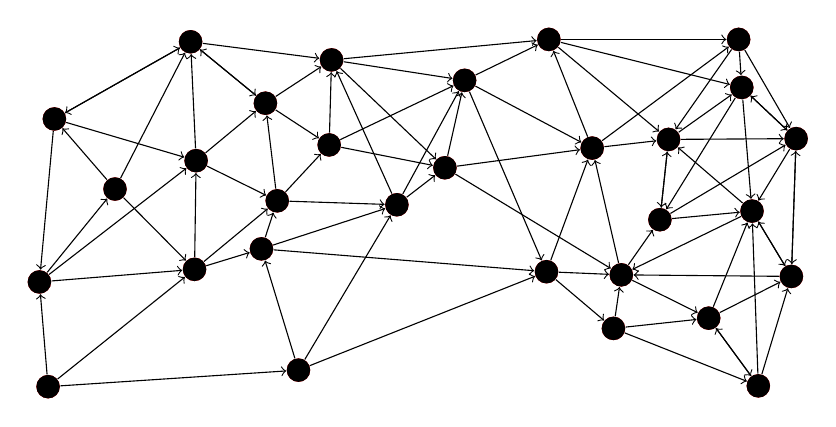
\begin{tikzpicture}
            \tikzstyle{before}=[circle,fill=black!20,inner sep=3pt]
            \tikzstyle{active}=[circle,fill=red,inner sep=3pt]
            \tikzstyle{after}=[circle,fill=black,inner sep=3pt]
            \node [before] (a)  at (0.45, 0.16) {}; \node<1> [active] at (0.45, 0.16) {}; \node<2-> [after] at (0.45, 0.16) {};
            \node [before] (b)  at (0.34, 1.49) {}; \node<2> [active] at (0.34, 1.49) {}; \node<3-> [after] at (0.34, 1.49) {};
            \node [before] (c)  at (2.31, 1.65) {}; \node<2> [active] at (2.31, 1.65) {}; \node<3-> [after] at (2.31, 1.65) {};
            \node [before] (d)  at (3.63, 0.37) {}; \node<2> [active] at (3.63, 0.37) {}; \node<3-> [after] at (3.63, 0.37) {};
            \node [before] (e)  at (1.30, 2.67) {}; \node<3> [active] at (1.30, 2.67) {}; \node<4-> [after] at (1.30, 2.67) {};
            \node [before] (f)  at (2.33, 3.03) {}; \node<3> [active] at (2.33, 3.03) {}; \node<4-> [after] at (2.33, 3.03) {};
            \node [before] (g)  at (0.53, 3.56) {}; \node<4> [active] at (0.53, 3.56) {}; \node<5-> [after] at (0.53, 3.56) {};
            \node [before] (h)  at (2.26, 4.54) {}; \node<4> [active] at (2.26, 4.54) {}; \node<5-> [after] at (2.26, 4.54) {};
            \node [before] (i)  at (3.36, 2.52) {}; \node<3> [active] at (3.36, 2.52) {}; \node<4-> [after] at (3.36, 2.52) {};
            \node [before] (j)  at (3.16, 1.91) {}; \node<3> [active] at (3.16, 1.91) {}; \node<4-> [after] at (3.16, 1.91) {};
            \node [before] (k)  at (4.88, 2.47) {}; \node<3> [active] at (4.88, 2.47) {}; \node<4-> [after] at (4.88, 2.47) {};
            \node [before] (l)  at (6.78, 1.62) {}; \node<3> [active] at (6.78, 1.62) {}; \node<4-> [after] at (6.78, 1.62) {};
            \node [before] (m)  at (3.21, 3.76) {}; \node<4> [active] at (3.21, 3.76) {}; \node<5-> [after] at (3.21, 3.76) {};
            \node [before] (n)  at (4.02, 3.23) {}; \node<4> [active] at (4.02, 3.23) {}; \node<5-> [after] at (4.02, 3.23) {};
            \node [before] (o)  at (4.05, 4.31) {}; \node<4> [active] at (4.05, 4.31) {}; \node<5-> [after] at (4.05, 4.31) {};
            \node [before] (p)  at (5.74, 4.05) {}; \node<4> [active] at (5.74, 4.05) {}; \node<5-> [after] at (5.74, 4.05) {};
            \node [before] (q)  at (5.49, 2.94) {}; \node<4> [active] at (5.49, 2.94) {}; \node<5-> [after] at (5.49, 2.94) {};
            \node [before] (r)  at (7.36, 3.19) {}; \node<4> [active] at (7.36, 3.19) {}; \node<5-> [after] at (7.36, 3.19) {};
            \node [before] (s)  at (7.73, 1.58) {}; \node<4> [active] at (7.73, 1.58) {}; \node<5-> [after] at (7.73, 1.58) {};
            \node [before] (t)  at (7.63, 0.90) {}; \node<4> [active] at (7.63, 0.90) {}; \node<5-> [after] at (7.63, 0.90) {};
            \node [before] (u)  at (6.81, 4.57) {}; \node<5> [active] at (6.81, 4.57) {}; \node<6-> [after] at (6.81, 4.57) {};
            \node [before] (v)  at (9.22, 4.57) {}; \node<5> [active] at (9.22, 4.57) {}; \node<6-> [after] at (9.22, 4.57) {};
            \node [before] (w)  at (8.33, 3.30) {}; \node<5> [active] at (8.33, 3.30) {}; \node<6-> [after] at (8.33, 3.30) {};
            \node [before] (x)  at (8.22, 2.28) {}; \node<5> [active] at (8.22, 2.28) {}; \node<6-> [after] at (8.22, 2.28) {};
            \node [before] (y)  at (8.84, 1.03) {}; \node<5> [active] at (8.84, 1.03) {}; \node<6-> [after] at (8.84, 1.03) {};
            \node [before] (z)  at (9.47, 0.17) {}; \node<5> [active] at (9.47, 0.17) {}; \node<6-> [after] at (9.47, 0.17) {};
            \node [before] (aa) at (9.26, 3.96) {}; \node<6> [active] at (9.26, 3.96) {}; \node<7-> [after] at (9.26, 3.96) {};
            \node [before] (bb) at (9.95, 3.31) {}; \node<6> [active] at (9.95, 3.31) {}; \node<7-> [after] at (9.95, 3.31) {};
            \node [before] (cc) at (9.39, 2.39) {}; \node<6> [active] at (9.39, 2.39) {}; \node<7-> [after] at (9.39, 2.39) {};
            \node [before] (dd) at (9.89, 1.56) {}; \node<6> [active] at (9.89, 1.56) {}; \node<7-> [after] at (9.89, 1.56) {};

            % Round 1
            \draw<1> [->] (a) -- (b);
            \draw<1> [->] (a) -- (c);
            \draw<1> [->] (a) -- (d);
            % Round 2
            \draw<2> [->] (b) -- (e);
            \draw<2> [->] (b) -- (c);
            \draw<2> [->] (b) -- (f);
            \draw<2> [->] (c) -- (f);
            \draw<2> [->] (c) -- (i);
            \draw<2> [->] (c) -- (j);
            \draw<2> [->] (d) -- (j);
            \draw<2> [->] (d) -- (k);
            \draw<2> [->] (d) -- (l);
            % Round 3
            \draw<3> [->] (e) -- (g);
            \draw<3> [->] (e) -- (h);
            \draw<3> [->] (e) -- (c);
            \draw<3> [->] (f) -- (h);
            \draw<3> [->] (f) -- (m);
            \draw<3> [->] (f) -- (i);
            \draw<3> [->] (i) -- (m);
            \draw<3> [->] (i) -- (n);
            \draw<3> [->] (i) -- (k);
            \draw<3> [->] (j) -- (i);
            \draw<3> [->] (j) -- (k);
            \draw<3> [->] (j) -- (l);
            \draw<3> [->] (k) -- (o);
            \draw<3> [->] (k) -- (p);
            \draw<3> [->] (k) -- (q);
            \draw<3> [->] (l) -- (r);
            \draw<3> [->] (l) -- (s);
            \draw<3> [->] (l) -- (t);
            % Round 4
            \draw<4> [->] (g) -- (b);
            \draw<4> [->] (g) -- (f);
            \draw<4> [->] (g) -- (h);
            \draw<4> [->] (h) -- (g);
            \draw<4> [->] (h) -- (m);
            \draw<4> [->] (h) -- (o);
            \draw<4> [->] (m) -- (h);
            \draw<4> [->] (m) -- (o);
            \draw<4> [->] (m) -- (n);
            \draw<4> [->] (n) -- (o);
            \draw<4> [->] (n) -- (p);
            \draw<4> [->] (n) -- (q);
            \draw<4> [->] (o) -- (u);
            \draw<4> [->] (o) -- (p);
            \draw<4> [->] (o) -- (q);
            \draw<4> [->] (p) -- (u);
            \draw<4> [->] (p) -- (r);
            \draw<4> [->] (p) -- (l);
            \draw<4> [->] (q) -- (p);
            \draw<4> [->] (q) -- (r);
            \draw<4> [->] (q) -- (s);
            \draw<4> [->] (r) -- (u);
            \draw<4> [->] (r) -- (v);
            \draw<4> [->] (r) -- (w);
            \draw<4> [->] (s) -- (r);
            \draw<4> [->] (s) -- (x);
            \draw<4> [->] (s) -- (y);
            \draw<4> [->] (t) -- (s);
            \draw<4> [->] (t) -- (y);
            \draw<4> [->] (t) -- (z);
            % Round 5
            \draw<5> [->] (u) -- (v);
            \draw<5> [->] (u) -- (aa);
            \draw<5> [->] (u) -- (w);
            \draw<5> [->] (v) -- (w);
            \draw<5> [->] (v) -- (aa);
            \draw<5> [->] (v) -- (bb);
            \draw<5> [->] (w) -- (aa);
            \draw<5> [->] (w) -- (bb);
            \draw<5> [->] (w) -- (x);
            \draw<5> [->] (x) -- (w);
            \draw<5> [->] (x) -- (bb);
            \draw<5> [->] (x) -- (cc);
            \draw<5> [->] (y) -- (cc);
            \draw<5> [->] (y) -- (dd);
            \draw<5> [->] (y) -- (z);
            \draw<5> [->] (z) -- (y);
            \draw<5> [->] (z) -- (cc);
            \draw<5> [->] (z) -- (dd);
            % Round 6
            \draw<6> [->] (aa) -- (bb);
            \draw<6> [->] (aa) -- (cc);
            \draw<6> [->] (aa) -- (x);
            \draw<6> [->] (bb) -- (aa);
            \draw<6> [->] (bb) -- (dd);
            \draw<6> [->] (bb) -- (cc);
            \draw<6> [->] (cc) -- (w);
            \draw<6> [->] (cc) -- (s);
            \draw<6> [->] (cc) -- (dd);
            \draw<6> [->] (dd) -- (bb);
            \draw<6> [->] (dd) -- (cc);
            \draw<6> [->] (dd) -- (s);
        \end{tikzpicture}
    \end{center}%
    \uncover<7>{Eventually reaches all nodes (with high probability).}
\end{frame}
\inlineslide{s:gossip}\label{l:gossip}


\section{Replication}\label{sec:replication}

\section{Work in progress from here onwards}


Distributed systems are fascinating because we have to work with partial knowledge and uncertain
truths. We never have certainty about the state of the system, because by the time we hear about
something, that state may already be outdated. In this way it resembles real life more than most of
computing! In real life you need to often make decisions with incomplete information.


Calendar app supports offline reads and writes (short video in airplane mode).

Fundamental building blocks of distributed systems: replication and partitioning.

Replication on one node: RAID-1. Geo-replication when replicas are geographically distributed

Replication example: two clients A and B, four servers. Server 1 receives only A's request,
server 2 receives A then B, server 3 receives B then A, and server 4 receives only B.
How do we ensure replicas become consistent with each other?

ABD algorithm. Last writer wins. Linearizability. Even shared memory on one machine is not linearisable!

CAP: consistent or available in the presence of a partition

Exercise. Show how to implement total order broadcast using Lamport timestamps [2020P5Q8]. Comment on its fault-tolerance properties.

% 1. Network communication basics: JSON, TCP, HTTP/REST, UDP. Hands-on: using things like tcpdump?
% 2. Faults and failures; failure detection; split brain
% 3. Architectures: client-server, local networks (multicast), peer-to-peer (distributed hash tables, NAT traversal)
% 4. Programming models: services, RPC, message brokers, actors, map-reduce, stream processing, tuple spaces?
% 5. Replication
% 6. Consensus
% 7. Convergence
% 8. Time and clocks
% 9. Security (e.g. TLS), byzantine fault tolerance, and blockchains

% Live demo of RESTful API with Dropwizard, curl, browser access

% State machine replication

% Define total order broadcast as:
% 1. If a correct process delivers message m, then m was broadcast by a process in the system.
% 2. No message is delivered more than once.
% 3. If a correct process p broadcasts a message m, then p eventually delivers m.
% 4. If a correct process delivers a message m, then all correct processes eventually deliver m.
% 5. If a correct process delivers m1 before delivering message m2, then all correct processes must deliver m1 before m2.
% Exercise: can't we combine properties 3 and 4 into one property, namely: if a correct process broadcasts a message m, then all correct processes eventually deliver m.
% Answer: no, this is not equivalent. Say message m is broadcast by faulty process p, and delivered by correct process q. In the original properties, m must now be delivered by all correct processes because it was delivered by one correct process. In the revised property, other processes would not necessarily need to deliver m, because it was sent by a faulty process.

% message loss -> retry; duplicates -> detect and suppress duplicates / idempotence
% idempotence: f(f(x)) = f(x)
% incrementing number of likes on a post: not idempotent
% adding current user to the set of users who have liked a post: idempotent
% what state must a recipient maintain in order to eliminate duplicates?
% the entire message? a unique message ID? a sequence number? (what assumptions does this require making about the sender?)
% Gossip protocols for replication / dissemination

% http://book.mixu.net/distsys/single-page.html
% BaseDS: https://github.com/vaidehijoshi/baseds-series  /   https://medium.com/baseds
% MIT graduate dist-sys course https://pdos.csail.mit.edu/6.824/schedule.html
% Raft animations: http://thesecretlivesofdata.com/raft/

% Beamer documentation:
% https://people.wou.edu/~beavers/LaTeX/beamer_guide.pdf
% http://anorien.csc.warwick.ac.uk/mirrors/CTAN/macros/latex/contrib/beamer/doc/beameruserguide.pdf

\bibliographystyle{plainnat}
\bibliography{references}{}
\end{document}
